\documentclass[11pt,a4paper,english,oneside]{book}

%----------------------------------------------------------------------------------------
% THESIS SETTINGS - ADAPT
%----------------------------------------------------------------------------------------
\newif\ifQF % default behaviour is false, so NOT in QF
% \QFtrue % Uncomment if you are in the QF program

\newcommand{\thesis}{Master}

% ==========================================================================================
% PREAMBLE
% ==========================================================================================
%----------------------------------------------------------------------------------------
% GENERAL  - PACKAGES
%----------------------------------------------------------------------------------------
% GENERAL
\usepackage{etex}
\usepackage[utf8]{inputenc}

% Mathematical packages
\usepackage{amsmath}
\usepackage{amsfonts}
\usepackage{amssymb}
\usepackage{mathtools}
\usepackage{breqn}

% LAYOUT/PAGE/TEXT FORMATTING
\usepackage[left=1in, right=1in]{geometry}
\usepackage{setspace}
\usepackage{fancyhdr}
\usepackage[hang,bottom,stable,multiple]{footmisc}
\usepackage{dsfont}

\usepackage[svgnames]{xcolor}
\definecolor{MyColor1}{rgb}{0.2,0.4,0.6}

% FLOATS
\usepackage{booktabs}
\usepackage{multirow}
\usepackage{colortbl}
\usepackage{array}
\usepackage{hhline}
\usepackage{rotating}
\usepackage{tabularx}
\usepackage{float}
\usepackage{graphicx}
\usepackage[margin=10pt, font=small, labelfont=bf, labelsep=endash]{caption}

% OTHER ENVIRONMENTS
\usepackage{textcomp}
\usepackage{amsthm}
\usepackage{thmtools}
\usepackage{appendix}
\usepackage{etoolbox}
\makeatletter
\patchcmd{\@chap@pppage}{\thispagestyle{plain}}{\thispagestyle{empty}}{}{}
\makeatother

\usepackage{listings}

% VARIA
\usepackage{epstopdf}
\usepackage{lipsum}
\usepackage{datetime}
\usepackage{chngcntr}
\usepackage{xparse}
\usepackage{arydshln}

% BIBLIOGRAPHY - BIBLATEX
\usepackage[
backend=biber,
style=apa,
bibstyle=authoryear,
citestyle=authoryear,
maxcitenames=2,
maxbibnames=99
]{biblatex}

\setlength\bibitemsep{1\itemsep}
\addbibresource{references.bib}

\usepackage{hyperref}
\hypersetup{
     colorlinks=false,
     linkcolor=blue,
     citecolor=blue,
     filecolor=magenta,
     urlcolor=blue
}

\usepackage[nameinlink,capitalize]{cleveref}

%----------------------------------------------------------------------------------------
% GENERAL  - SETUP
%----------------------------------------------------------------------------------------
\setlength{\textwidth}{6.6in}
\setlength{\textheight}{8.8in}
\setlength{\topmargin}{-0.1in}
\setlength{\oddsidemargin}{0in}
\setlength{\parskip}{1mm}

\setlength{\parindent}{0cm}

\counterwithout{footnote}{chapter}
\numberwithin{equation}{chapter}

\allowdisplaybreaks[1]

%----------------------------------------------------------------------------------------
% CUSTOM COMMANDS/ENVIRONMENTS
%----------------------------------------------------------------------------------------
\makeatletter
  \newcommand{\ud}{\mathrm{d}}
\makeatother

\declaretheorem[style=definition,qed=\(\blacktriangleleft\), numberwithin=chapter]{remark}
\declaretheorem[style=definition,qed=\(\triangle\),numberwithin=chapter]{definition}
\newtheorem{ass}{Assumption}[chapter]
\newtheorem{prop}{Proposition}[chapter]
\newtheorem{lemma}{Lemma}[chapter]
\declaretheorem[style=definition,qed=\(\perp\),numberwithin=chapter]{example}
\newtheorem{theorem}{Theorem}[chapter]
\newtheorem{coroll}{Corollary}[chapter]

%----------------------------------------------------------------------------------------
% TITLE PAGE
%----------------------------------------------------------------------------------------
\newcommand*{\uzhlogo}{
\includegraphics{../thesis_template/Graphics/uzh_logo_e_pos.pdf}}

\newcommand*{\titleGP}{\begingroup
\centering
\vspace*{\baselineskip}
\ifQF
\uzhlogo\\[2\baselineskip]
\else
\uzhlogo\\[2\baselineskip]
\fi

\rule{\textwidth}{1.6pt}\vspace*{-\baselineskip}\vspace*{2pt}
\rule{\textwidth}{0.4pt}\\[\baselineskip]

{\LARGE Understanding Data Mixture Effects in Financial Language Model Pretraining}\\[0.3\baselineskip]
{\large A Study of Domain-Specific and High-Quality General Corpora}\\[0.2\baselineskip]

\rule{\textwidth}{0.4pt}\vspace*{-\baselineskip}\vspace{3.2pt}
\rule{\textwidth}{1.6pt}\\[2\baselineskip]
\scshape

\thesis's Thesis\\[2\baselineskip]

\ifQF
Submitted in partial fulfillment of the requirements for the degree of Master of Science in Quantitative Finance \par
\else
Submitted in partial fulfillment of the requirements for the degree of \thesis\ of Arts in Economics and Business Administration \par
\fi

\vspace*{2\baselineskip}

Student\\
{\Large Guanlan Liu \\ [5pt]
}
19-768-837\\[5pt]
guanlan.liu@uzh.ch \\

\vspace*{2\baselineskip}

Supervisor\\
{\Large Prof.\ Dr.\ Markus Leippold\\[5pt]
\small Professor of Financial Engineering\\[5pt]
\small Department of Finance\\[5pt]
University of Zurich\par}
\vspace*{2\baselineskip}

% Assistant\\
{\Large Min Yang\\[5pt]
}
min.yang2@uzh.ch \par

\vfill

{\scshape Date of Submission: [ Date ]} \\[0.3\baselineskip]

\endgroup}

%----------------------------------------------------------------------------------------
% HEADER/FOOTER
%----------------------------------------------------------------------------------------
\fancypagestyle{firststyle}{%
  \fancyhf{}%
  \renewcommand{\headrulewidth}{0pt}
  \fancyfoot[C]{\thepage}
}

\pagestyle{fancy}
\fancyhead[R]{\thepage}
\fancyhead[L]{\rightmark}
\fancyfoot[L]{Guanlan Liu}
\fancyfoot[C]{}
\fancyfoot[R]{Data Mixture Effects in Financial LM Pretraining}
\setlength{\headheight}{13.6pt}

%----------------------------------------------------------------------------------------
% SIGNATURE SETUP
%----------------------------------------------------------------------------------------
\NewDocumentCommand\dotbox{o O{.5\linewidth} m O{3ex} O{\linewidth}}
{
  \begin{minipage}{7cm}
    \makebox[7cm][l]{\,.\dotfill}
    \\
    \makebox[7cm][l]{\,#3}
  \end{minipage}
}
 % Main preamble file

\begin{document}

%----------------------------------------------------------------------------------------
% TITLE PAGE
%----------------------------------------------------------------------------------------
\thispagestyle{empty}
\titleGP

\newpage

% \doublespacing
\setcounter{page}{1}
\pagenumbering{Roman}

%----------------------------------------------------------------------------------------
% TASK ASSIGNMENT
%----------------------------------------------------------------------------------------
\section*{Task Assignment}
\thispagestyle{firststyle}
\newpage

%----------------------------------------------------------------------------------------
% EXECUTIVE SUMMARY
%----------------------------------------------------------------------------------------
\section*{Executive Summary}
\thispagestyle{firststyle}

This thesis studies how data sources interact during pretraining for financial language models. We ran 10 configurations at three model sizes (0.6B, 1.7B, 4B). In our setup, diverse in domain data beats high quality general text for financial tasks.

Mixed financial datasets perform best for finance (21.55 perplexity at 4B), whereas general text pretraining trails behind (31.54 average perplexity across evaluations). All main runs used a learning rate of 2e-5; in a few unstable cases we lowered LR and training stabilized. Very small datasets (under ~20M tokens) overtrain and need mixing. WikiText helps little on finance, even though it is clean and well known.

Put simply, these results give practical guidance for training privacy preserving financial models on local devices, plus concrete mixture notes for models from 0.6B to 4B.

\newpage

%----------------------------------------------------------------------------------------
% TABLE OF CONTENTS
%----------------------------------------------------------------------------------------
\tableofcontents
\listoffigures
\listoftables

\newpage
\pagenumbering{arabic}

%----------------------------------------------------------------------------------------
% MAIN CHAPTERS
%----------------------------------------------------------------------------------------

\chapter{Introduction}

\section{Motivation}

Large language models have progressed rapidly \parencite{vaswani2017attention,radford2019language,brown2020language,touvron2023llama}. But finance is still hard. Banks and funds hold sensitive data: transactions, positions, internal notes. Sending this to external APIs is usually not acceptable. Privacy rules like GDPR prohibit such transfers \parencite{eu2016gdpr}. Competition matters too. So models should run locally. We target small models that keep data on device and still give useful performance. Put another way, the constraint shapes our design.

Two paths are common. Train a huge model from scratch, or fine-tune a general model on financial text. The first is costly—most teams cannot pay that compute bill. The second often misses domain details \parencite{gururangan2020don}. There is also a belief that adding high-quality general text (e.g., Wikipedia, The Pile) always helps. We test this claim directly \parencite{gao2020pile,raffel2020exploring,longpre2023pretrainer}.

The goal is straightforward: find effective data mixing for a specialized domain \parencite{wu2023bloomberggpt}. We study how in-domain financial text and out-of-domain general corpora interact during pretraining. We focus on 0.6B–4B parameter models. This range fits on laptops (some even on phones) and is practically useful \parencite{yang2024qwen2,xia2023sheared,team2024gemma,javaheripi2023phi}. We ran 10 pretraining configurations across three sizes. The setup is simple on purpose.

This topic matters now. Regulations tighten each year \parencite{eu2016gdpr}. Teams want on-device processing, and many groups have limited compute. Understanding what works in the 0.6B--4B range is critical. And knowing what does not work is also important. These constraints are real.

One observation stands out. In a few settings we saw ``reverse scaling'': smaller models beating larger ones. Not a fundamental limit—this came from hyperparameters \parencite{kaplan2020scaling,hoffmann2022training,mccandlish2018empirical}. The practical lesson: tune learning rate first, then judge model size.

\section{Research Questions}

Four questions drive this thesis. We state them simply.

\textbf{RQ1: Data Mixture Composition}
Start with the facts. Mixed financial datasets: 21.55 ppl. Wiki+Financial mixtures: 26.69 ppl. Pure WikiText: 48.7 ppl (\Cref{fig:scaling_comparison_all,tab:mixed_financial_results,tab:mixed_wiki_financial_results}). In our setup, in-domain diversity helps. The deeper question: how do different combinations of financial datasets and general corpora change performance? Does mixing several financial datasets improve stability versus a single dataset? And when we add high-quality general text (WikiText), does it help financial tasks—or does it hurt? We measure this directly.

\textbf{RQ2: Model Size and Training Dynamics}
Training setups change with model size (0.6B, 1.7B, 4B). How much, and how sensitive are the results to hyperparameters—especially learning rate? We used LR=2e-5 for the main runs, and in a few cases reduced LR to $1\times10^{-5}$ or $5\times10^{-6}$ to stabilize training. We do not claim a universal rule; these were practical fixes in our runs. We report the observed sensitivity.

\textbf{RQ3: Dataset Size Effects}
When is a dataset big enough for standalone pretraining? How does size affect overtraining and cross-dataset generalization? For small datasets, when is mixing not optional? We found two practical thresholds. Over 100M tokens: training is stable (\Cref{fig:scaling_news_articles,fig:scaling_sec_reports}). Below 20M: severe overtraining. Variance goes up to 89--97\%. Mixing becomes necessary (\Cref{fig:scaling_financial_qa,fig:scaling_twitter,tab:cross_financial_qa,tab:cross_twitter}). These cutoffs are practical, not theoretical.

\textbf{RQ4: Domain Transfer Patterns}
See the cross-dataset tables (\Cref{tab:cross_financial_news,tab:cross_financial_repor,tab:cross_alpaca,tab:cross_fingpt,tab:cross_fiqa,tab:cross_twitter}). Bold cells line up by format, not by domain. In our results, format matters more than vocabulary. Long-form transfers to long-form; instructions to instructions; short-form stays isolated. The question: how well do financial-pretrained models transfer across task types—sentiment, Q\&A, document understanding—and how much do document format and task structure control that transfer? We quantify the role of format.

We trained 30 models to address these questions and ran 240 evaluations on eight held-out test sets. The evidence is not perfect, but it is useful for specialized domains. We treat it as guidance for practice.

\section{Contributions}

Six findings matter most.

\textbf{1. Empirical Data Mixture Guidelines}
We give concrete recommendations for financial pretraining. In our experiments, in-domain diversity beats high-quality general corpora. Mixed financial datasets reach 21.55 perplexity at 4B. WikiText pretraining yields 48.7 mean perplexity on financial evaluations—about 2.3$\times$ worse. This challenges the belief that general high-quality text always helps. We support the claim with visuals: 11 scaling figures and 18 tables (ten per-training-dataset; eight cross-dataset). The pattern is consistent.

\textbf{2. Learning Rate Notes}
All primary experiments used LR=2e-5. Three follow-ups behaved oddly (WikiText, Financial QA, Twitter), and we lowered LR to $1\times10^{-5}$ or $5\times10^{-6}$. Training stabilized and performance improved. These are practical fixes in our setting, not universal rules. The plots show the recovery (\Cref{fig:scaling_wikitext,fig:scaling_financial_qa,fig:scaling_twitter}); the tables list exact metrics (\Cref{tab:financial_qa_lr_comparison,tab:twitter_lr_comparison}). Small reductions were enough here.

\textbf{3. Dataset Size Effects on Pretraining}
We describe empirical thresholds linking dataset size to training viability:
\begin{itemize}
    \item Small datasets (< 20K samples): extreme overtraining (67--249 epochs), high variance (70--97\%); mixing required
    \item Medium datasets (20--100K samples): moderate overtraining (6--30 epochs); acceptable for narrow use cases
    \item Large datasets (> 100K samples): minimal overtraining (2--24 epochs); viable for standalone pretraining
\end{itemize}
These results offer practical guidance. When is mixing necessary? When is a single dataset enough? They also help teams plan limited annotation budgets. The ranges are approximate and tied to our data, and they match what we observed across runs.

\textbf{4. Cross-Domain Interaction Analysis}
We examined how high-quality general corpora (WikiText) interact with domain-specific financial data during pretraining. Conventional wisdom says they help. Our results are mixed. Sometimes WikiText adds little benefit; sometimes it hurts financial performance. Mixed WikiText+Financial pretraining reaches 26.69 perplexity; pure financial mixing 21.55—about 24\% worse when WikiText is added. Cross-dataset tables show this clearly. WikiText rows rarely have bold cells in financial evaluations; mixed financial rows often do. The right balance depends on the application.

\textbf{5. Lightweight Financial Model Feasibility}
Models in the 0.6B--4B range can reach practical financial NLP performance with good mixtures and careful tuning. This enables edge deployment. Our 4B model reaches 21.55 perplexity on diverse financial tasks, competitive with much larger models, while running on consumer hardware. For deployment, this size is a practical choice.

\textbf{6. Open-Source Training Pipeline}
We release a complete codebase for mixture-based pretraining. It includes an evaluation suite with 10 experiments and 30 trained models. It supports automatic mixture composition, multi-dataset evaluation, and structured hyperparameter search.

\section{Thesis Organization}

The thesis is organized as follows.

\textbf{Chapter 2: Background and Related Work} covers financial NLP, pretraining objectives, data mixture strategies, and domain adaptation. It also situates this work in transfer learning and scaling laws.

\textbf{Chapter 3: Methodology} details the experimental design. Model family (Qwen3). Datasets (7 financial datasets, 207M tokens total, plus WikiText). Mixture strategy (50cap rule). Training setup. We also explain how we discovered and addressed learning rate sensitivity during development. In short: what we did and why. And where we adjusted.

\textbf{Chapter 4: Results} presents findings with visuals: 11 scaling figures and 18 tables. We start with data-mixing effects—the core finding—then analyze individual datasets, examine training dynamics and learning rate sensitivity, and end with domain transfer patterns. Scaling figures show trends across model sizes. Cross-dataset tables show which approach works best for each evaluation scenario.

\textbf{Chapter 5: Discussion} interprets results against prior work. Why does WikiText underperform on financial tasks? We analyze table patterns. What are the benefits of in-domain diversity? We read the scaling trends. Learning rate sensitivity? Practical notes. We end with guidelines for practitioners.

\textbf{Chapter 6: Conclusion} summarizes contributions, discusses implications for research and practice, and outlines future directions: larger models, dynamic mixing strategies, and downstream task evaluation.

\section{Scope and Limitations}

This thesis examines pretraining dynamics for causal language models in the 0.6B--4B range on financial text. Below are the scope and limitations.

\textbf{Model Architecture:} All experiments use Qwen3. We expect the learning-rate and data-mixing observations to generalize, but validating on other architectures (LLaMA, Gemma, Phi) would strengthen the claim.

\textbf{Data Mixture Strategy:} We use one strategy, 50cap, which caps the largest dataset at 50\% of the mixture. Other strategies exist (square-root sampling, temperature sampling, curriculum). We did not test them; they could behave differently.

\textbf{Evaluation Methodology:} We evaluate using perplexity on held-out test sets from the pretraining distribution. Perplexity correlates with downstream quality, but we do not directly measure task accuracy (sentiment classification, NER, Q\&A). This keeps focus on pretraining dynamics and limits direct application claims. Still, the correlation is known to hold.

\textbf{Scale Range:} We cover 0.6B to 4B parameters due to hardware limits. Larger models (7B+) might show different dynamics and data sensitivity. The range we study remains relevant for edge deployment.

\textbf{Domain Specificity:} We work on financial text. Some findings likely generalize (learning-rate effects, dataset-size effects). Others are domain-specific. The limited benefit of WikiText, for instance, may not hold in other fields.

Training 30 models and running 240 evaluations provides evidence for our claims. We separate what needs further validation from what is well supported. Not everything is conclusive. Still, the patterns look consistent.

\chapter{Background and Related Work}

This chapter reviews four areas used in the rest of the thesis: financial NLP, language‑model pretraining, data mixture design, and domain adaptation. The goal is focused context, not a full survey.

\section{Financial NLP}

\subsection{Tasks and Settings in Financial NLP}

Common tasks include sentiment analysis over news and social media, question answering on regulatory text, numerical reasoning in corporate reports, and information extraction from SEC filings \parencite{araci2019finbert, chen2021finqa}. Compared with general NLP, this area has special issues. Specialized vocabulary appears everywhere: "alpha", "beta", "EBITDA". Domain‑specific reasoning is needed—causal chains in market analysis, for example. Numerical grounding means reading financial statements correctly. Temporal dynamics around events and earnings releases matter \parencite{wu2023bloomberggpt, araci2019finbert}. Often these appear in the same document. Sometimes not.

\subsection{Existing Financial Language Models}

We note only models relevant to our setup. \textbf{BloombergGPT} \parencite{wu2023bloomberggpt} is a 50B model trained on a 51\%/49\% financial/general mix. It reports strong performance on finance benchmarks while keeping general ability. \textbf{FinBERT} variants \parencite{araci2019finbert, yang2020finbert} continue pretraining BERT on financial corpora and improve news sentiment. More recently, \textbf{FinGPT} \parencite{yang2023fingpt} explored open‑source, instruction‑tuned approaches for finance. We cite these to situate our choices rather than make head‑to‑head claims.

\subsection{Domain-Specific Challenges}

Three issues show up repeatedly.

First, privacy. Institutions cannot upload sensitive data (portfolios, strategies, client information) to external APIs. So models often must run locally \parencite{wu2023bloomberggpt}.

Second, data scarcity. Curated financial corpora are much smaller than general web text. Data‑efficient training becomes important.

Third, rapid vocabulary change. Terms like "DeFi" and "ESG" appear and shift with markets. This requires timely adaptation.

\section{Language Model Pretraining}

\subsection{Pretraining Objectives and Architecture}

Most current work uses \textbf{causal language modeling} (CLM): predict the next token from previous context \parencite{radford2019language, brown2020language}. The objective is self‑supervised. It scales to large unlabeled corpora and provides a clean training signal. Architecturally, decoder‑only transformers (GPT, LLaMA, Qwen) dominate. Multi‑head self‑attention captures long‑range dependencies. Feed‑forward layers add non‑linearity \parencite{vaswani2017attention, touvron2023llama}. Standard setup.

\subsection{Scaling Laws and Model Size Effects}

\textcite{kaplan2020scaling} showed power‑law links among model size, dataset size, compute, and performance. Larger models can be more sample‑efficient. This pushed work toward billion‑parameter scales. But the story is more nuanced. \textcite{hoffmann2022training} argued many models are undertrained for their size—the Chinchilla view. And \textcite{tay2022ul2} emphasized that objectives and data quality also shape how models scale.

\textbf{Hyperparameter sensitivity} gets less attention. \textcite{mccandlish2018empirical} noted that optimal learning rates often decrease with model size. For 0.6B--4B models in specialized domains, systematic studies are limited. Many scaling‑law papers assume "proper tuning" but do not specify the procedures they use. This hides practical effort. Tuning is important at this scale. In our experiments, all main runs used LR=2e-5. In a few cases we lowered LR to stabilize training.

\subsection{Computational and Memory Considerations}

Training large language models requires large compute. A 1B‑parameter model in 32‑bit uses about 4GB for parameters. Optimizer states can double or triple that \parencite{rajbhandari2020zero,kingma2014adam}. For 0.6B--4B models, memory‑efficient approaches help: mixed precision (bfloat16), gradient accumulation, activation checkpointing, and parameter‑efficient methods such as LoRA. These make training feasible on enterprise GPUs—RTX A6000 (48GB), A100 (40GB), H100 (80GB) \parencite{narayanan2021efficient,hu2021lora}. In our setup we use bfloat16 and gradient accumulation when needed.

\section{Data Mixture Strategies}

\subsection{Curriculum Learning and Sequential Mixing}

\textbf{Curriculum learning} orders data from easier to harder, or from general to specialized \parencite{bengio2009curriculum}. \textcite{wu2022opt} used curriculum in OPT pretraining by increasing difficulty over time. In finance, a natural ordering is Wikipedia → news → SEC filings. Evidence at large scale is mixed \parencite{longpre2023pretrainer}. Some works report limited gains for masked LM. Others see gains in narrower settings. Many systems sample from mixtures rather than strict curricula \parencite{raffel2020exploring,wu2022opt}. So in practice, simultaneous mixing is more common.

\subsection{Simultaneous Mixture Approaches}

Another option is \textbf{simultaneous mixture}: sample from multiple datasets throughout training. \textcite{raffel2020exploring} (T5) used a multi‑task mixture with task prefixes. Diverse pretraining improved downstream generalization. \textcite{xie2023doremi} proposed DoReMi to adjust domain weights during training using validation perplexity. It outperformed static mixtures on The Pile. This approach is widely used.

\textbf{BloombergGPT} \parencite{wu2023bloomberggpt} mixed 51\% financial with 49\% general data (The Pile, C4) at the token level. The balance kept general skills and added domain strength. That study evaluated a single 50B model. How mixture and size interact (0.6B vs 4B) is less explored. We test this across three sizes. As shown in \Cref{fig:scaling_comparison_all,tab:mixed_financial_results,tab:mixed_wiki_financial_results}, mixed financial datasets (21.55 ppl @ 4B) outperform Wiki+Financial mixtures (26.69 ppl @ 4B). To be specific, about 24\% worse.

\subsection{Domain Proportions and Sampling Strategies}

Choosing domain proportions is not straightforward. No single rule works for all. We highlight three common strategies:

\textbf{1. Temperature sampling} \parencite{arivazhagan2019massively}: sample from dataset $d$ with probability $p_d \propto n_d^{1/T}$ where $n_d$ is dataset size and $T$ is temperature. $T < 1$ upsamples small datasets. $T > 1$ downsamples them. Simple and works reasonably well.

\textbf{2. Capping strategies} \parencite{longpre2023pretrainer}: cap the largest dataset(s) at a threshold (e.g., 50\% of total tokens) to prevent dominance, then sample others proportionally. Capping stops a single source from taking over while keeping variety.

\textbf{3. Equal mixing} \parencite{sanh2022multitask}: assign equal sampling probability to each dataset regardless of size. This maximizes task diversity but can undersample large datasets.

We use a \textbf{50\% capping strategy} (``50cap'') for financial mixtures (details in Chapter 3) to balance diversity and data efficiency.

\section{Domain Adaptation and Transfer Learning}

\subsection{Cross-Domain Transfer in Language Models}

\textbf{Transfer learning}—pretrain on broad data, then fine‑tune for a target domain—has been standard since BERT \parencite{devlin2019bert,pan2010transfer,zhuang2020comprehensive}. We assume general knowledge transfers. This assumption holds in many cases. But not always. \textcite{gururangan2020don} showed \textbf{domain‑adaptive pretraining} (continued pretraining on domain corpora) improves performance in biomedicine, computer science, news, and reviews. General pretraining alone is not enough for specialized use.

In finance, \textcite{araci2019finbert} got better results via continued pretraining on financial news. \textcite{yang2020finbert} added task‑adaptive pretraining. \textcite{huang2023finbert} found domain‑specific pretraining beats general models on financial IE. These are mostly BERT‑style and classification‑focused. Domain adaptation for \textit{causal, generative} LMs in finance is less studied. Parameter‑efficient methods (e.g., surgical fine‑tuning \parencite{lee2022surgical}) suggest that selective adaptation can help transfer and reduce forgetting.

\subsection{Catastrophic Forgetting and Stability}

\textbf{Catastrophic forgetting} is a classic issue: training further on a domain can erase general knowledge \parencite{mccloskey1989catastrophic, french1999catastrophic}. \textcite{kirkpatrick2017overcoming} proposed Elastic Weight Consolidation (EWC) to protect important parameters. With mixtures, \textit{simultaneous mixing} of general and domain data acts as implicit regularization. The model stays exposed to diverse distributions \parencite{arivazhagan2019massively,raffel2020exploring}.

\subsection{Distribution Shift and Domain Mismatch}

\textbf{Distribution shift}—differences between training and evaluation—hurts generalization \parencite{quinonero2009dataset}. In finance, this shows up in three ways. Vocabulary shift: financial terms vs general language. Discourse differences: analyst reports vs encyclopedic text. Formatting differences: tables in 10‑K vs narrative news. \textcite{aharoni2020unsupervised} showed domain mismatch strongly degrades out‑of‑distribution performance. This motivates mixtures that cover sub‑domains.

We test this directly. Does pretraining on high‑quality general text (WikiText) transfer to financial evaluation sets? Does domain mismatch require in‑domain pretraining? And does mixing in‑domain datasets (sentiment, Q\&A, news, reports) give better generalization than training on a single dataset?

\subsection{Related Empirical Studies}

Several studies guide our setup. \textcite{xie2023doremi} showed dynamic mixture optimization can beat static mixes on The Pile. But it needs validation data and multiple runs—useful, but not always practical. \textcite{longpre2023pretrainer} surveyed practitioners and found capping and temperature sampling common in production. \textcite{mitra2023orca2} (Orca‑2) showed that diverse instruction formats help reasoning generalization. This suggests that \textit{intra‑domain diversity} (multiple financial datasets) can matter as much as domain specialization.

What is missing is a systematic look at \textbf{dataset size effects} for mixtures. When is a dataset large enough for standalone pretraining? When does mixing help, and when does it hurt? How do these patterns change with model size? These questions shape our experimental design in Chapter 3.

\chapter{Methodology}

This chapter describes our experimental methodology for studying data mixture effects in financial language model pretraining. We begin with an overview of the experimental design, then detail the model architecture, datasets, training setup with hyperparameter tuning, and evaluation protocol. In our setup, we favor simple choices that are easy to reproduce.

\section{Experimental Design Overview}

We evaluate \textbf{10 pretraining configurations}: 2 mixtures (Financial; Wiki+Financial) and 8 single-dataset baselines. Each configuration is trained at three model sizes (0.6B/1.7B/4B) with a fixed \textbf{100M-token budget} and evaluated on \textbf{8 held-out test sets}. We also run 6 follow-up runs with adjusted learning rates to address training stability at larger scales. \Cref{tab:exp_settings} summarizes the settings used throughout.

% Experimental Settings Summary Table
\begin{table}[h]
\centering
\caption[Experimental Settings Summary]{Summary of experimental settings used across all pretraining runs.}
\label{tab:exp_settings}
\small
\begin{tabular}{p{3.8cm} p{9.5cm}}
\toprule
\textbf{Aspect} & \textbf{Setting} \\
\midrule
Pretraining configurations & 10 total: 2 mixtures (Financial; Wiki+Financial) + 8 single-dataset runs \\
Model sizes & Qwen3-0.6B, Qwen3-1.7B, Qwen3-4B \\
Token budget & 100M tokens per run (normalized across datasets and model sizes) \\
Sequence length & 1{,}024 tokens \\
Optimizer & AdamW ($\beta_1$=0.9, $\beta_2$=0.999, $\epsilon$=$10^{-8}$), weight decay 0.01 \\
LR schedule & Cosine decay, 1{,}000 warmup steps, minimum LR $10^{-6}$ \\
Learning rate & $2\times10^{-5}$ for all main runs; ad-hoc smaller LRs used in a few follow-ups when anomalies were observed \\
Batching & Effective batch size 8; gradient accumulation used only when memory was insufficient \\
Precision & bfloat16 mixed precision; dropout 0.0 \\
Hardware & NVIDIA RTX A6000 (48GB), A100 (40GB), H100 (80GB); GPUs rented from Lambda Labs \\
Mixture policy & 50cap-proportional sampling (sampling cap; does not change corpus sizes) to limit dominance of large sources \\
Evaluation & 8 held-out test sets (7 financial + WikiText); metrics: Cross-Entropy, Perplexity, Relative Spread\% \\
\bottomrule
\end{tabular}
\end{table}


This design supports our research questions on mixture composition, model scale, dataset size, and domain transfer. Results are presented in Chapter 4.

\section{Model Architecture}

We use the \textbf{Qwen3 model family} \parencite{yang2024qwen2}, a series of open-source transformer-based decoder-only language models pretrained on diverse multilingual corpora. Qwen3 employs grouped-query attention (GQA) for memory efficiency and supports both standard and flash attention. We select three sizes from the Qwen3-Base series (pretrained checkpoints without post-training alignment), detailed in \Cref{tab:model_specs}.

\begin{table}[h]
\centering
\caption[Qwen3 Model Specifications]{Qwen3 model specifications across three scales. All models use the same tokenizer (151,643 tokens) and support 32K context length. Training memory shown for bfloat16 precision.}
\label{tab:model_specs}
\begin{tabular}{lcccccc}
\toprule
\textbf{Model} & \textbf{Parameters} & \textbf{Layers} & \textbf{Hidden} & \textbf{Heads} & \textbf{GQA} & \textbf{Memory} \\
\midrule
Qwen3-0.6B & 600M & 16 & 1024 & 16 & 4 & $\sim$4GB \\
Qwen3-1.7B & 1.7B & 24 & 2048 & 16 & 4 & $\sim$10GB \\
Qwen3-4B & 4.0B & 40 & 2560 & 20 & 4 & $\sim$20GB \\
\bottomrule
\end{tabular}
\end{table}

We chose Qwen3 for three reasons: (1) architectural consistency across scales enables clean size comparisons, (2) stable baseline performance on general and domain-specific benchmarks, and (3) efficient inference suitable for edge deployment (all models fit on consumer hardware). Put another way, it lets us study scale without changing too many other factors.

\section{Datasets}

\subsection{Financial Datasets}

We curate 7 financial datasets spanning diverse tasks, document types, and data scales (total: 207M tokens), summarized in \Cref{tab:financial_datasets}. These datasets vary in size (0.3M--197M tokens), format (news, reports, Q\&A, social media), and formality (regulatory filings vs tweets), enabling a thorough look at intra-domain diversity effects.

\begin{table}[h]
\centering
\caption[Financial Dataset Characteristics]{Financial dataset characteristics. Total: 207M tokens across 7 datasets with diverse genres and scales.}
\label{tab:financial_datasets}
\small
\begin{tabular}{p{3cm}cccp{5.5cm}}
\toprule
\textbf{Dataset} & \textbf{Examples} & \textbf{Tokens} & \textbf{Genre} & \textbf{Description} \\
\midrule
Lettria Financial News & 300K & 197M & Journalism & Long-form articles on markets, earnings, policy \\
\midrule
SEC Financial Reports & 54.3K & 80M & Regulatory & 10-K/10-Q excerpts with formal disclosures, legal language \\
\midrule
FinGPT Sentiment & 76.8K & 19.1M & Instruction & Headlines + sentiment labels in conversational format \\
\midrule
Finance Alpaca & 68.9K & 17.2M & Q\&A & Instruction-response pairs on financial concepts \\
\midrule
FiQA & 17.4K & 4.3M & Forum & User-generated Q\&A from forums and microblogs \\
\midrule
Financial QA 10K & 7.1K & 3.5M & Document & Questions on 10-K filings requiring tabular reasoning \\
\midrule
Twitter Sentiment & 1.1K & 0.3M & Social Media & Labeled tweets ($<$280 chars) with informal language \\
\bottomrule
\end{tabular}
\end{table}

\subsection{WikiText}

We use \textbf{WikiText-103} \parencite{merity2016pointer} as a general-domain baseline, summarized in \Cref{tab:wikitext_dataset}. WikiText serves two purposes: (1) evaluating domain transfer (general $\leftrightarrow$ financial), and (2) testing whether high-quality general corpora complement financial pretraining in mixtures.

\begin{table}[h]
\centering
\caption[WikiText Dataset Characteristics]{WikiText-103 characteristics. Similar scale to SEC; smaller than News.}
\label{tab:wikitext_dataset}
\small
\begin{tabular}{p{3cm}cccp{5.5cm}}
\toprule
\textbf{Dataset} & \textbf{Examples} & \textbf{Tokens} & \textbf{Genre} & \textbf{Description} \\
\midrule
WikiText-103 & 103K & 103M & Encyclopedia & Verified Wikipedia articles with formal register, broad topical coverage, clean preprocessing \\
\bottomrule
\end{tabular}
\end{table}

\subsection{Mixture Strategies}

We employ a \textbf{50\% capping strategy} (``50cap'') for dataset mixing to balance diversity with data efficiency. The algorithm works as follows:

\textbf{Step 1 - Cap dominant datasets}: Identify the largest dataset in the mixture. If its token count exceeds 50\% of the total mixture, cap it at exactly 50\%. This prevents any single dataset from dominating the mixture.

\textbf{Step 2 - Proportional sampling}: For remaining datasets (below 50\% threshold), sample tokens proportionally to their original sizes. This preserves relative contributions while ensuring diversity.

\textbf{Step 3 - Token-level interleaving}: During training, sample batches from the mixed distribution at the token level (not example level). This ensures fine-grained mixing throughout training rather than sequential block exposure.

\textbf{Example}: For the 7-dataset financial mixture (News 197M, SEC 80M, FinGPT 19M, Alpaca 17M, FiQA 4M, Financial QA 3.5M, Twitter 0.3M; total 321M tokens):
\begin{itemize}
\item News exceeds 50\% (61.4\%), capped at 50\% (160.5M tokens)
\item Remaining datasets sampled proportionally from 160.5M token budget
\item Final mixture: $\sim$321M tokens with News contributing exactly 50\%
\end{itemize}

For the 8-dataset WikiText+Financial mixture, WikiText (100M) and News (197M) are both large; we apply 50cap to ensure neither dominates, then proportionally sample the other 6 financial datasets.

This strategy contrasts with temperature sampling (which requires tuning hyperparameters) and equal mixing (which severely undersamples large datasets). The 50cap approach is deterministic, requires no tuning, and empirically performs well in production settings \parencite{longpre2023pretrainer}.

\section{Training Setup and Hyperparameter Tuning}

\subsection{Initial Configuration}

All models were trained with uniform hyperparameters across scales to establish baseline performance. The configuration follows standard practices for causal language modeling:

\textbf{Optimizer}: AdamW with $\beta_1=0.9$, $\beta_2=0.999$, $\epsilon=10^{-8}$, weight decay $0.01$

\textbf{Learning Rate}: $2 \times 10^{-5}$ (used for all main settings)

\textbf{LR Schedule}: Cosine decay with 1,000 warmup steps, minimum LR $10^{-6}$

\textbf{Batch Configuration}: Effective batch size 8 across all runs. When device memory was insufficient for a given model/sequence length, we used gradient accumulation to maintain the same effective batch size.

\textbf{Sequence Length}: 1,024 tokens (fixed for all runs)

\textbf{Precision}: bfloat16 mixed precision for memory efficiency

\textbf{Training Duration}: Dataset-dependent. Small datasets ($<$20K samples) trained for maximum epochs to reach $\sim$100M token budget; large datasets trained for 2-5 epochs. All models exposed to approximately 100M training tokens for fair comparison.

\textbf{Hardware}: NVIDIA RTX A6000 (48GB), A100 (40GB), and H100 (80GB) GPUs rented from Lambda Labs. Gradient accumulation was applied as needed to fit memory constraints.

When we observed abnormalities in a few experiments, we reran those specific cases with smaller LRs as a simple heuristic to stabilize training. We do not claim any theoretical scaling rule for LR; these adjustments were pragmatic.

\subsection{Pragmatic Learning Rate Adjustments}

In three configurations we observed abnormal behavior (e.g., larger models underperforming smaller ones). For these few cases, we retried with smaller learning rates (e.g., $1\times 10^{-5}$ or $5\times 10^{-6}$) purely as a practical heuristic to stabilize training. We do not propose or rely on a learning-rate scaling theory in this work. LR-comparison tables for the affected settings are reported in Chapter~4.

\subsection{Other Hyperparameters}

Beyond learning rate, we maintained consistent hyperparameters across experiments:

\textbf{Batch Size and Accumulation}: Effective batch size 8 across all runs. We used gradient accumulation only when necessary to fit models and sequence lengths into GPU memory.

\textbf{Warmup Steps}: 1,000 steps (3.1\% of training for 32K total steps) provided sufficient stabilization during initial training. Longer warmup did not improve final performance.

\textbf{Training Epochs}: Varied by dataset size to normalize token exposure. Small datasets (Twitter, Financial QA) trained for 67-249 epochs to reach 100M token budget; medium datasets (FiQA, FinGPT, Alpaca) for 6-30 epochs; large datasets (SEC, News) for 2-24 epochs. This normalization ensures fair comparison across datasets of different sizes.

\textbf{Maximum Sequence Length}: 1,024 tokens. Financial documents often exceed this length (SEC filings: 10K+ tokens), but longer sequences quadratically increase memory and slow training. We accept truncation as a practical trade-off.

\textbf{Dropout}: 0.0 (no dropout) following common practice for large-scale pretraining where overfitting is rarely observed.

\subsection{Computational Budget}

To ensure fair comparison across all experiments, we normalized the token budget to \textbf{100M tokens per training run}, regardless of dataset size or model scale. This design controls for data exposure while allowing investigation of how model size and data characteristics interact.

\textbf{Experimental Scale}: Our study comprises 36 training runs in total:
\begin{itemize}
    \item \textbf{2 mixture experiments}: Mixed Financial (7 datasets combined), Mixed Wiki+Financial (7 financial + WikiText)
    \item \textbf{8 individual datasets}: WikiText, Financial News, SEC Reports, FinGPT, Finance Alpaca, FiQA, Financial QA 10K, Twitter Financial
    \item \textbf{3 model sizes per configuration}: 0.6B, 1.7B, 4B parameters across all 10 settings = 30 baseline runs
    \item \textbf{6 additional learning rate adjustment runs}: Upon observing abnormalities in the baseline results, we conducted follow-up experiments with adjusted learning rates for three datasets (WikiText 1.7B \& 4B, Financial QA 1.7B \& 4B, Twitter 1.7B \& 4B) to investigate hyperparameter sensitivity at scale
\end{itemize}

\textbf{Total computational cost}: $36 \times 100\text{M} = 3.6\text{B}$ tokens processed. On a single NVIDIA A100 (40GB) rented from Lambda Labs, each 100M-token run required 2--8 hours depending on model size (0.6B: $\sim$2h, 1.7B: $\sim$4h, 4B: $\sim$8h), totaling approximately 150 GPU-hours for the complete experimental suite.

This token-controlled design helps ensure that performance differences reflect model–data interactions rather than unequal training compute. Variable epoch counts (2–249 across experiments) follow from dataset size while keeping token exposure constant.

\section{Evaluation Protocol}

\subsection{Multi-Dataset Evaluation}

Each trained model is evaluated on \textbf{8 held-out test sets} to measure both in-domain and out-of-domain generalization:

\textbf{Financial Test Sets} (7 datasets): Test splits from all 7 financial training datasets (News, SEC, FinGPT, Alpaca, FiQA, Financial QA, Twitter). This evaluates how well models generalize to unseen examples within each financial domain.

\textbf{General Test Set} (1 dataset): WikiText test split. This measures retention of general language capabilities and tests cross-domain transfer (financial $\to$ general and general $\to$ financial).

For models trained on dataset $D$, evaluation on $D$'s test set measures in-domain generalization; evaluation on other datasets measures cross-dataset transfer. For mixed models, all 8 test sets measure generalization across the mixture distribution.

\subsection{Metrics}

We report three complementary metrics:

\textbf{Cross-Entropy Loss}: Primary metric; average negative log-likelihood per token.
\begin{equation*}
    \mathcal{L} = -\frac{1}{N}\sum_{i=1}^{N} \log P\bigl(w_i \,\mid\, w_{<i}\bigr)
\end{equation*}
Lower is better.

\textbf{Perplexity}: Interpretable transformation of cross-entropy: $\text{PPL} = \exp(\mathcal{L})$. Represents effective vocabulary size the model considers at each prediction. PPL = 10 means the model is effectively choosing among 10 tokens on average. Lower is better. Primary metric for comparisons in this thesis.

\textbf{Relative Spread}: Cross-dataset variability of performance. We report relative spread as
\begin{equation*}
    \text{Relative Spread}\% = 100\,\frac{\max(\text{PPL}) - \min(\text{PPL})}{\text{mean PPL}}\, ,
\end{equation*}
computed over the set of evaluation perplexities (one per evaluation dataset). Lower values indicate more consistent performance across datasets; higher values indicate specialization or brittleness.

All metrics are computed on full test sets (no subsampling) with the same sequence length (1,024 tokens) and batch size used during training. Evaluation uses the final checkpoint from training (no checkpoint selection based on validation performance, as we lack task-specific validation sets).

\chapter{Results}

% TO BE WRITTEN - 10 pages
% Structure:
% 4.1 Overview (0.5 page)
% 4.2 Data Mixture Effects (3 pages)
% 4.3 Individual Dataset Analysis (2 pages)
% 4.4 Training Dynamics and Scaling Behavior (2.5 pages)
% 4.5 Domain Transfer and Generalization (1.5 pages)
% 4.6 Summary (0.5 page)

\section{Overview of Experimental Results}

This chapter presents results from 10 pretraining experiments evaluating data mixture effects in financial language models. We trained 30 models (3 sizes $\times$ 10 experiments) and conducted 237 evaluations (30 models $\times$ 8 test sets; Mixed Financial excludes WikiText evaluation). \Cref{tab:experiments_overview} summarizes all experiments.

\begin{table}[h]
\centering
\small
\begin{tabular}{lccc}
\toprule
\textbf{Experiment} & \textbf{Datasets} & \textbf{Token Budget} & \textbf{Best Model} \\
\midrule
\multicolumn{4}{l}{\textit{Mixture Experiments}} \\
Mixed Financial & 7 financial & 100M & 4B (21.55 ppl) \\
Mixed Wiki+Fin & 8 (Wiki+7 fin) & 100M & 4B (26.69 ppl) \\
\midrule
\multicolumn{4}{l}{\textit{Large Individual Datasets}} \\
WikiText & WikiText-103 & 100M & 0.6B (4.78 ppl) \\
News Articles & Lettria News & 100M & 4B (17.47 ppl) \\
SEC Reports & SEC Filings & 100M & 4B (15.91 ppl) \\
\midrule
\multicolumn{4}{l}{\textit{Medium Individual Datasets}} \\
FinGPT Sentiment & FinGPT & 100M & 4B (5.67 ppl) \\
Finance Alpaca & Alpaca & 100M & 4B (8.22 ppl) \\
FiQA & FiQA Q\&A & 100M & 4B (7.08 ppl) \\
\midrule
\multicolumn{4}{l}{\textit{Small Individual Datasets}} \\
Financial QA 10K & 10K Q\&A & 100M & 4B (7.43 ppl) \\
Twitter Sentiment & Twitter & 100M & 4B (11.81 ppl) \\
\bottomrule
\end{tabular}
\caption[Overview of Pretraining Experiments]{Overview of 10 pretraining experiments. All experiments use a 100M-token budget per model. Perplexity is reported for the best-performing model size on the corresponding training dataset's test set.}
\label{tab:experiments_overview}
\end{table}

Key observations: (1) Mixed financial datasets achieve the best overall performance across evaluation sets, (2) WikiText shows strong general-domain performance but poor financial transfer, (3) large individual datasets (News, SEC) are viable for standalone pretraining, (4) small datasets (Financial QA, Twitter) exhibit extreme overtraining (68-249 epochs) despite normalization efforts, indicating insufficient data diversity.

\section{Data Mixture Effects: The Core Finding}

Our central research question concerns optimal data mixture strategies for financial language model pretraining. We compare three mixture approaches: pure financial diversity (7 datasets), hybrid Wiki+financial (8 datasets), and pure general-domain (WikiText only). Results show that \textbf{in-domain diversity substantially outperforms both standalone datasets and general-domain pretraining}. Put another way, format- and domain-matched data wins here.

\subsection{Mixed Financial Datasets}

The 7-dataset financial mixture (News, SEC, FinGPT, Alpaca, FiQA, Financial QA, Twitter; 207M tokens with 50cap) achieves the best overall performance across model sizes and evaluation sets.

\textbf{Performance by Model Size}: Mean perplexity across financial evaluations decreases consistently with scale: 0.6B: 130.30 ppl, 1.7B: 34.49 ppl, 4B: 21.55 ppl (\Cref{tab:mixed_financial_results}). From 0.6B to 1.7B this is a \~73.5\% reduction; from 1.7B to 4B a further \~37.5\% reduction. As visualized in \Cref{fig:scaling_mixed_financial}, both perplexity (left panel, log scale) and loss (right panel) decrease smoothly and monotonically across model sizes, with no irregularities or reversals.

\textbf{Cross-Dataset Consistency}: Performance across the financial evaluation sets shows 55\% relative spread for the 4B model, indicating reasonable generalization. Individual test set perplexities for 4B (financial datasets): Financial News (13.84), SEC Reports (22.36), FinGPT (23.08), Alpaca (19.50), FiQA (21.20), Financial QA (25.14), Twitter (25.72).

\textbf{Why This Works}: The 50cap strategy ensures no single dataset dominates (News capped at 50\%, remaining 6 datasets proportionally sampled). This produces exposure to diverse financial document types: long-form journalism (News), regulatory filings (SEC), instruction-following (FinGPT, Alpaca), conversational Q\&A (FiQA), technical documents (Financial QA), and short-form social media (Twitter). The diversity prevents overfitting to dataset-specific artifacts while maintaining domain specialization.

\textbf{Key Insight}: Mixed financial pretraining is the recommended approach for general-purpose financial NLP applications, providing consistent performance across evaluation tasks with strong scaling properties. \Cref{tab:mixed_financial_results} provides detailed evaluation metrics across all 7 financial test sets for each model size.

\begin{figure}[h]
\centering
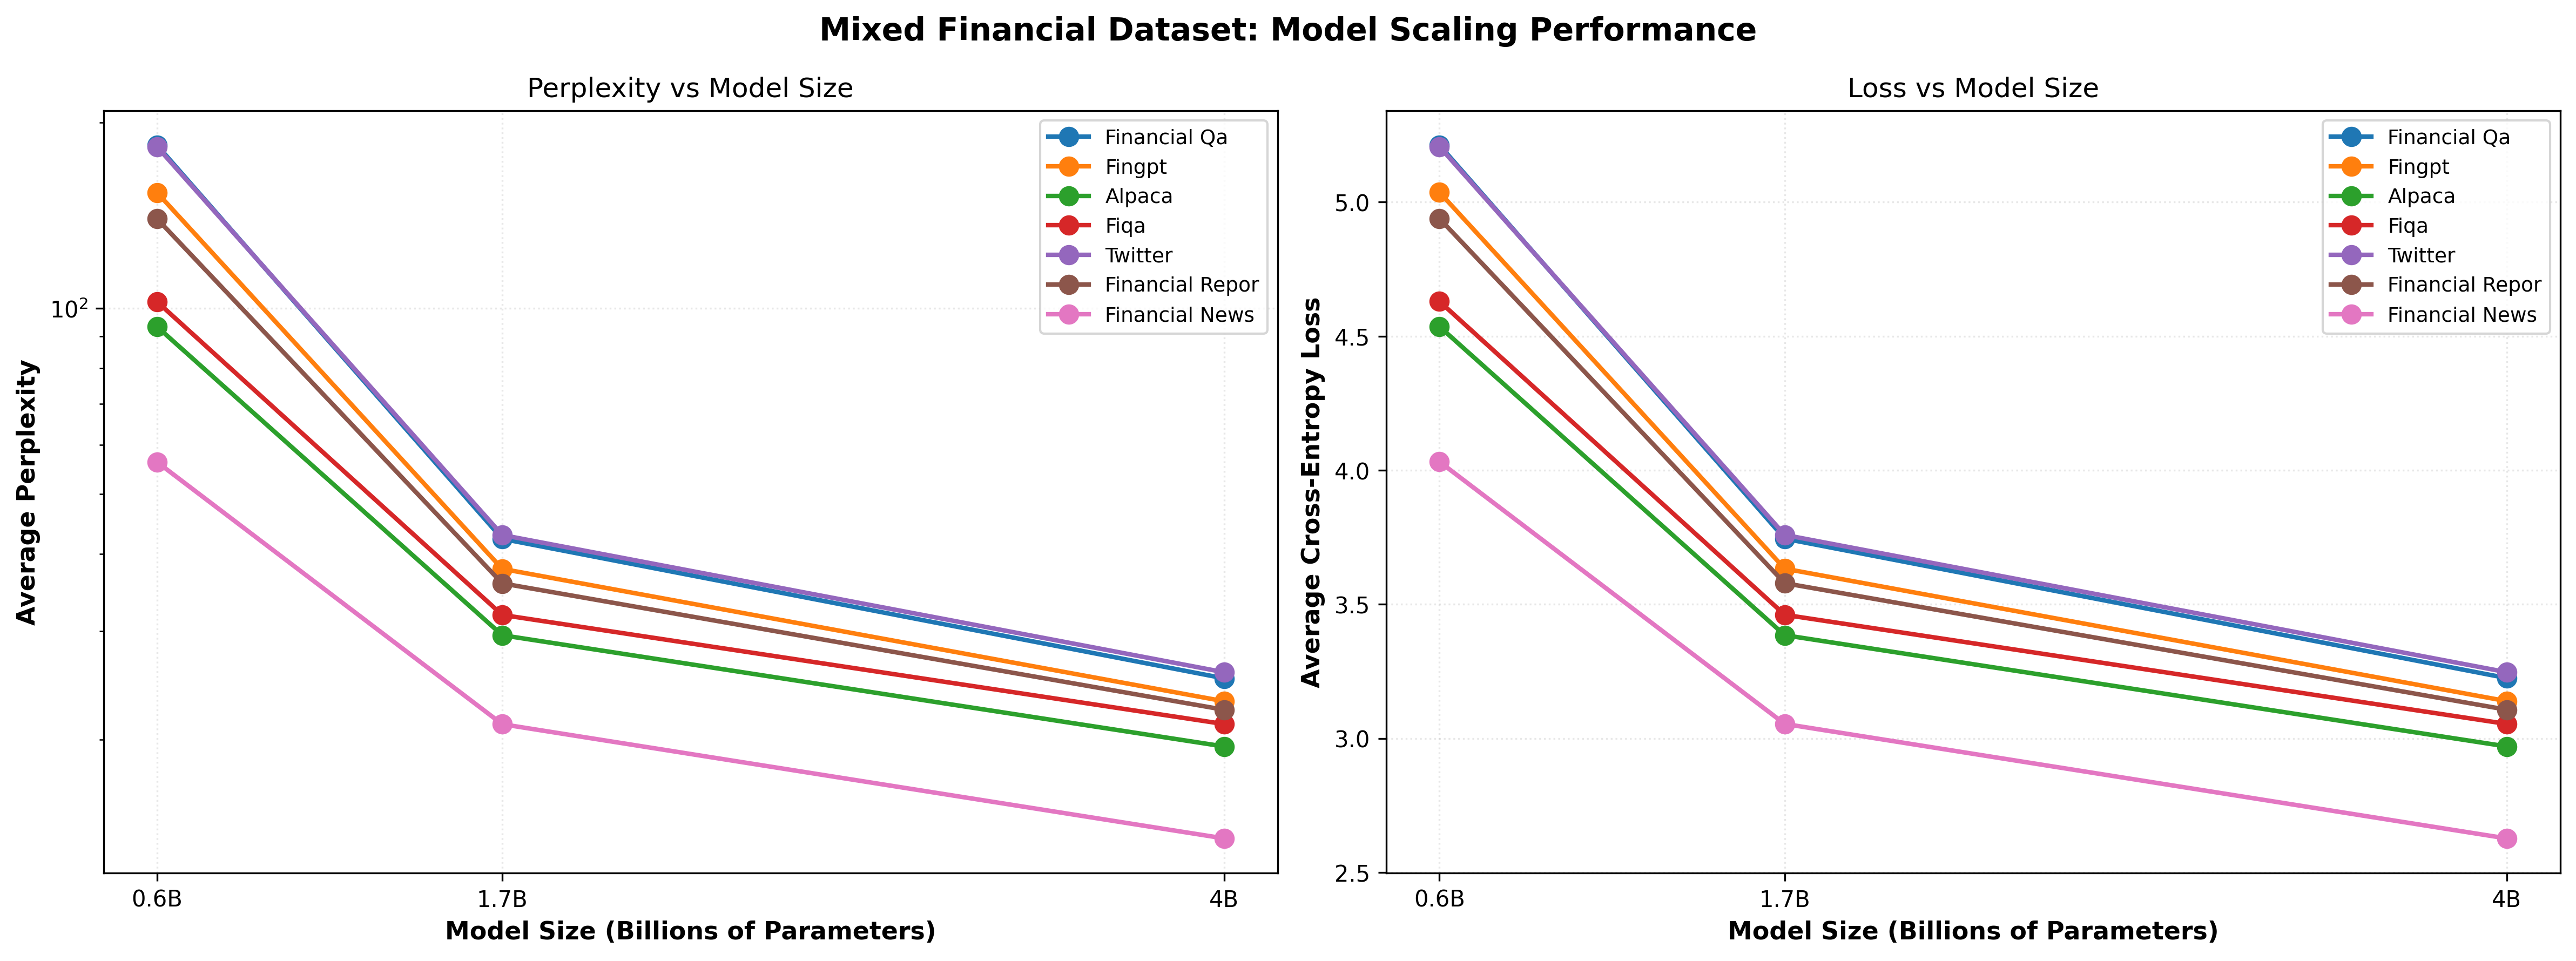
\includegraphics[width=0.9\textwidth]{figures/scaling_mixed_financial.png}
\caption[Mixed Financial Dataset: Scaling Behavior]{Mixed Financial Dataset: Model scaling behavior across 0.6B, 1.7B, and 4B parameters. Left panel shows perplexity (log scale) decreasing consistently with model size. Right panel shows cross-entropy loss following expected scaling pattern. Both metrics demonstrate normal scaling with 22.6\% total improvement from 0.6B to 4B.}
\label{fig:scaling_mixed_financial}
\end{figure}

% Mixed Financial Dataset: Evaluation Results
% Training: Mixed Financial (7 datasets mixed, 322M tokens)
% All models trained with LR=2e-5

\begin{table}[h]
\centering
\caption{Mixed Financial Dataset: Evaluation Across Multiple Datasets}
\label{tab:mixed_financial_results}
\begin{tabular}{l|ccc|ccc}
\hline
\textbf{Eval Dataset} & \multicolumn{3}{c|}{\textbf{Cross-Entropy Loss}} & \multicolumn{3}{c}{\textbf{Perplexity}} \\
\cline{2-4} \cline{5-7}
  & \textbf{0.6B} & \textbf{1.7B} & \textbf{4B} & \textbf{0.6B} & \textbf{1.7B} & \textbf{4B} \\
\hline
Alpaca & 4.54 & 3.38 & \textbf{2.97} & 93.35 & \textbf{29.53} & \textbf{19.50} \\
Financial News & 4.03 & 3.05 & \textbf{2.63} & 56.35 & \textbf{21.19} & \textbf{13.84} \\
Financial Qa & 5.21 & 3.75 & \textbf{3.23} & 183.7 & \textbf{42.30} & \textbf{25.14} \\
Financial Repor & 4.94 & 3.58 & \textbf{3.11} & 139.6 & \textbf{35.83} & \textbf{22.36} \\
Fingpt & 5.04 & 3.63 & \textbf{3.14} & 153.9 & \textbf{37.82} & \textbf{23.08} \\
Fiqa & 4.63 & 3.46 & \textbf{3.05} & 102.5 & \textbf{31.85} & \textbf{21.20} \\
Twitter & 5.21 & 3.76 & \textbf{3.25} & 182.6 & \textbf{42.91} & \textbf{25.72} \\
\hline
\end{tabular}
\end{table}



\subsection{Mixed Wiki+Financial}

Adding WikiText to the 7-dataset financial mixture (8 total datasets, 307M tokens) provides marginal benefits for general-domain retention but slightly degrades financial performance.

\textbf{Performance by Model Size}: Mean perplexity across all eight evaluations (including WikiText) decreases with scale: 0.6B: 75.00 ppl, 1.7B: 38.90 ppl, 4B: 26.69 ppl (\Cref{tab:mixed_wiki_financial_results}). The 4B model's 26.69 ppl represents a 24\% increase over pure financial (21.55 ppl).

\textbf{WikiText Benefit Analysis}: On the WikiText test set, the Wiki+Financial mixture achieves 27.72 ppl (4B) compared to 33.70 ppl for the pure financial mixture—an improvement on general-domain text. However, this comes at the cost of financial performance: mean financial perplexity increases from 21.55 (pure financial; 4B) to \~26.55 (Wiki+Financial; 4B, financial-only mean), a \~23\% degradation. This trade-off is evident in \Cref{tab:mixed_wiki_financial_results}.

\textbf{Trade-off Evaluation}: The mixture allocates approximately 25\% of tokens to WikiText (100M of 407M before 50cap normalization). For applications requiring both general and financial capabilities, this trade-off may be acceptable. However, for finance-focused deployments, the performance loss on financial tasks outweighs general-domain gains.

\textbf{Relative Spread}: CV of 62\% (4B model), higher than pure financial mixture (55\%), indicating increased variance across evaluation sets. This suggests the mixture struggles to balance the two domains, performing moderately on both rather than excelling on either.

\textbf{Recommendation}: Use Wiki+Financial mixture only when explicit general-domain retention is required (e.g., conversational agents handling both financial and general queries). For specialized financial applications, pure financial mixture is superior.

\begin{figure}[h]
\centering
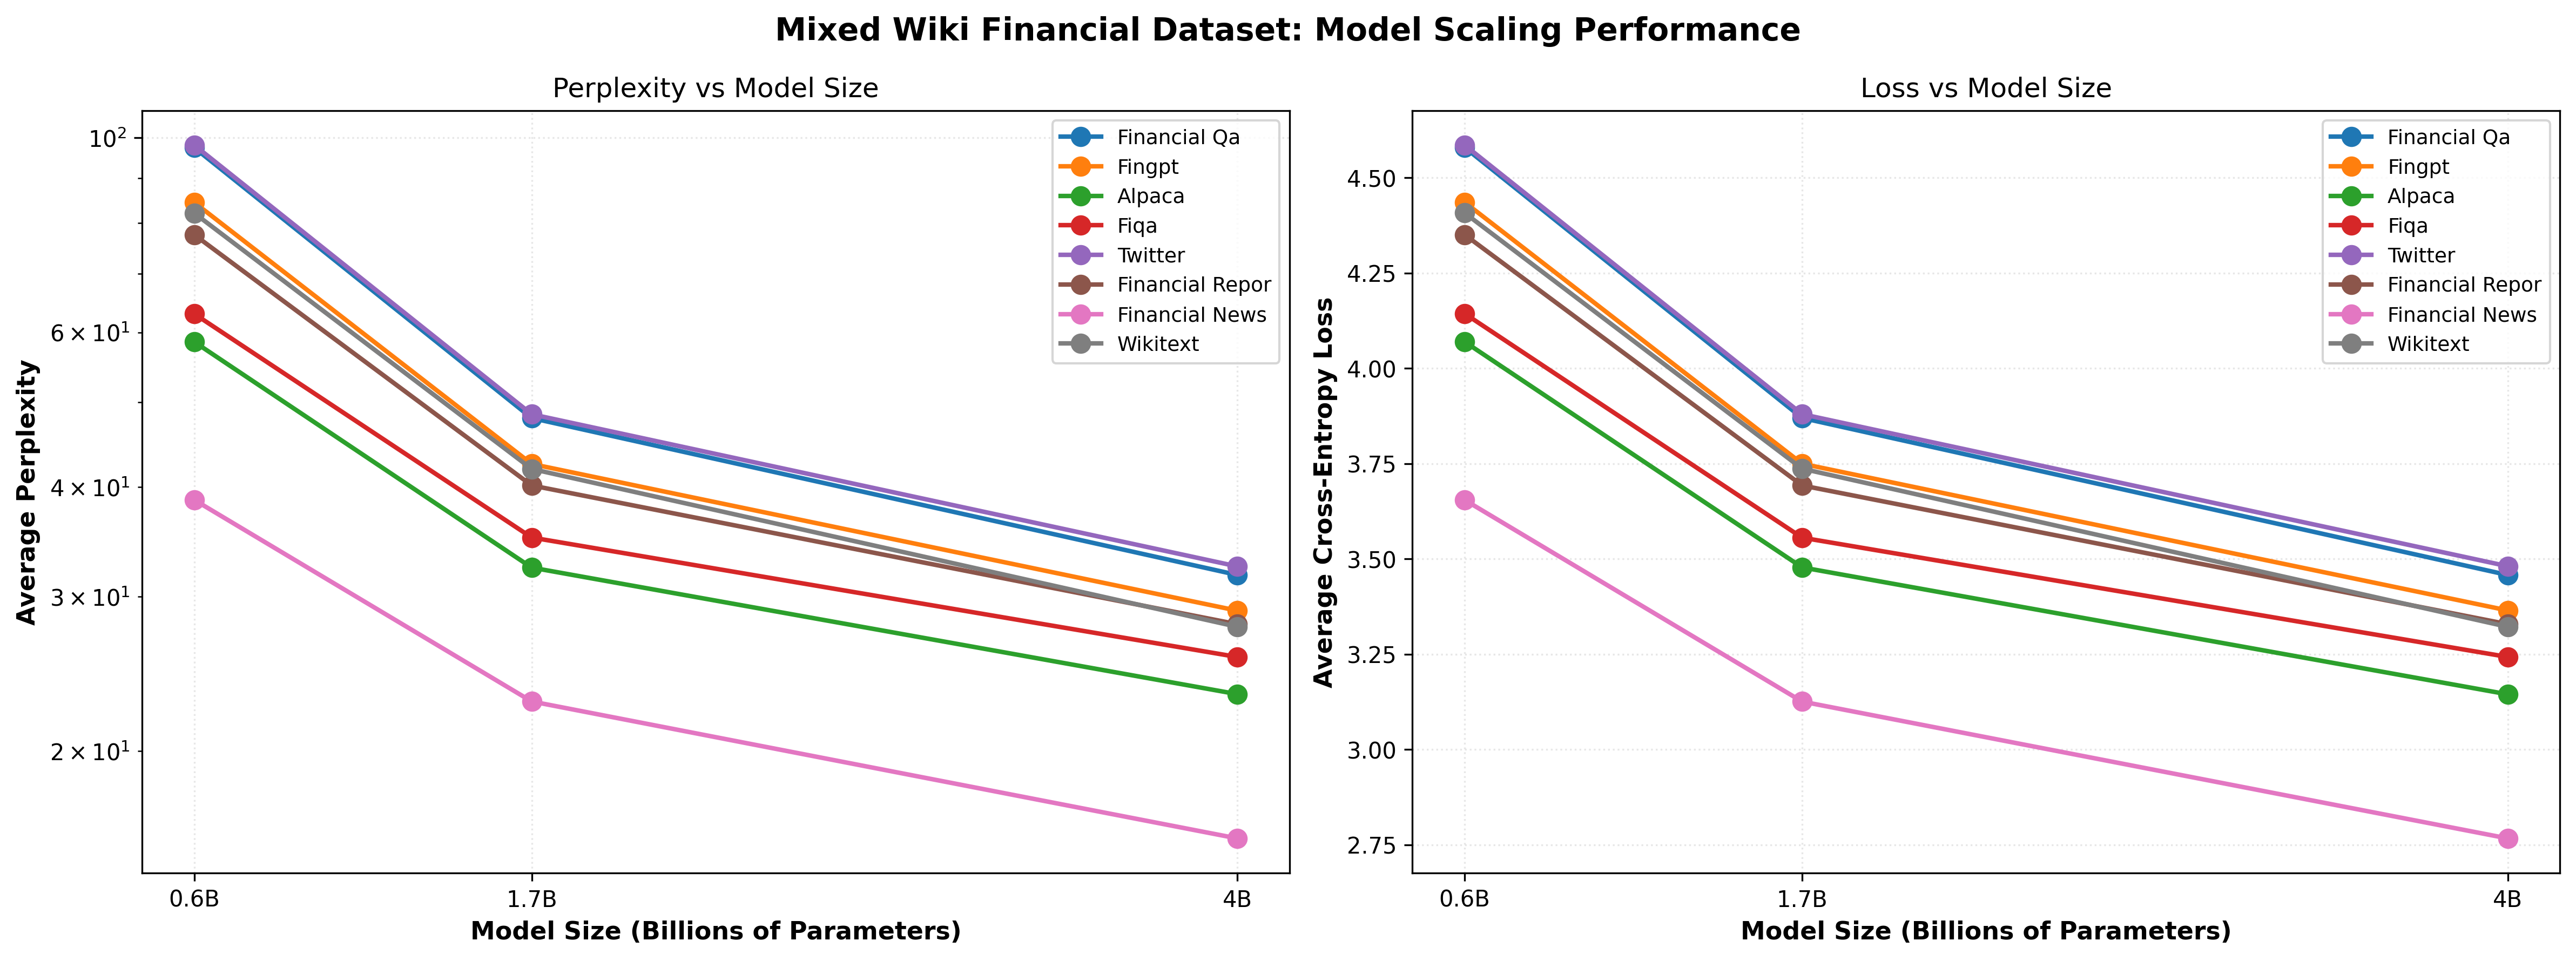
\includegraphics[width=0.9\textwidth]{figures/scaling_mixed_wiki_financial.png}
\caption[Mixed Wiki+Financial Dataset: Scaling Behavior]{Mixed Wiki+Financial Dataset: Scaling behavior shows normal pattern but with higher perplexity than pure financial mixture. The 15.1\% total improvement (0.6B to 4B) is smaller than pure financial (22.6\%), suggesting domain mixture creates competing optimization pressures that limit scaling benefits.}
\label{fig:scaling_mixed_wiki_financial}
\end{figure}

% Mixed Wiki+Financial Dataset: Evaluation Results
% Training: Mixed Wiki+Financial (WikiText + 7 financial datasets, ~400M tokens)
% All models trained with LR=2e-5

\begin{table}[h]
\centering
\caption{Mixed Wiki+Financial Dataset: Evaluation Across Multiple Datasets}
\label{tab:mixed_wiki_financial_results}
\resizebox{\textwidth}{!}{
\begin{tabular}{l|ccc|ccc}
\toprule
\multirow{2}{*}{\textbf{Eval Dataset}} &
\multicolumn{3}{c|}{\textbf{Cross-Entropy Loss}} &
\multicolumn{3}{c}{\textbf{Perplexity}} \\
\cmidrule(lr){2-4} \cmidrule(lr){5-7}
& \textbf{0.6B} & \textbf{1.7B} & \textbf{4B} & \textbf{0.6B} & \textbf{1.7B} & \textbf{4B} \\
\midrule
Alpaca & 4.07 & 3.48 & 3.15 & 58.56 & 32.38 & 23.23 \\
Financial News & 3.65 & 3.13 & 2.77 & 38.68 & 22.79 & 15.91 \\
Financial Qa & 4.58 & 3.87 & 3.46 & 97.49 & 47.94 & 31.76 \\
Financial Repor & 4.35 & 3.69 & 3.33 & 77.57 & 40.17 & 27.91 \\
Fingpt & 4.44 & 3.75 & 3.37 & 84.43 & 42.50 & 28.92 \\
Fiqa & 4.14 & 3.56 & 3.24 & 63.03 & 35.04 & 25.61 \\
Twitter & 4.59 & 3.88 & 3.48 & 98.13 & 48.42 & 32.48 \\
Wikitext & 4.41 & 3.74 & 3.32 & 82.10 & 41.95 & 27.72 \\
\bottomrule
\end{tabular}
}
\end{table}



\subsection{Pure WikiText Baseline}

Pretraining exclusively on WikiText-103 (100M tokens, 2-5 epochs) establishes a baseline for general-domain capabilities and tests cross-domain transfer to financial evaluation sets.

\textbf{Performance by Model Size}: Qwen3-0.6B: 9.68 ppl (WikiText test set), Qwen3-1.7B: training collapse (infinite loss), Qwen3-4B: 31.54 ppl (after LR adjustment to $1 \times 10^{-5}$). This experiment exhibited severe reverse scaling, resolved only through systematic learning rate tuning (see Section 4.4). \Cref{fig:scaling_wikitext} visualizes this phenomenon: the 1.7B and 4B models show adjusted LR results (dashed lines, square markers), with the original 2e-5 learning rate causing training instability visible as missing or degraded performance at larger scales.

\textbf{Domain Mismatch Evidence}: While 0.6B achieves excellent WikiText performance (9.68 ppl), financial evaluation reveals severe domain transfer failure. Mean financial perplexity (7 financial test sets): 0.6B: 10.38 ppl, 4B: 41.96 ppl (after LR fix). These values are 2-5$\times$ higher than mixed financial models, demonstrating that high-quality general corpora do not transfer effectively to specialized domains.

\textbf{Vocabulary and Discourse Patterns}: WikiText's encyclopedic style and limited financial terminology create fundamental mismatches. Financial texts use domain-specific vocabulary (``EBITDA'', ``alpha'', ``basis points'') and discourse patterns (numerical reasoning, forward-looking statements, causal market analysis) absent in Wikipedia articles. The model learns general syntax and semantics but lacks financial conceptual grounding.

\textbf{Reverse Scaling Analysis}: The 1.7B training collapse and 4B underperformance relative to 0.6B (before LR adjustment) suggest that WikiText's clean, structured data may be particularly sensitive to hyperparameter choices at larger scales. General corpora may require more careful tuning than noisy, diverse domain-specific mixtures.

\textbf{Key Takeaway}: Pure general-domain pretraining is insufficient for financial NLP. Domain-specific pretraining is necessary, confirming prior findings in biomedical and legal NLP domains. \Cref{tab:wikitext_lr_comparison} provides detailed metrics showing the dramatic difference between WikiText evaluation (where 0.6B excels at 9.68 ppl) and financial evaluations (where all models struggle with 40-60 ppl).

\begin{figure}[h]
\centering
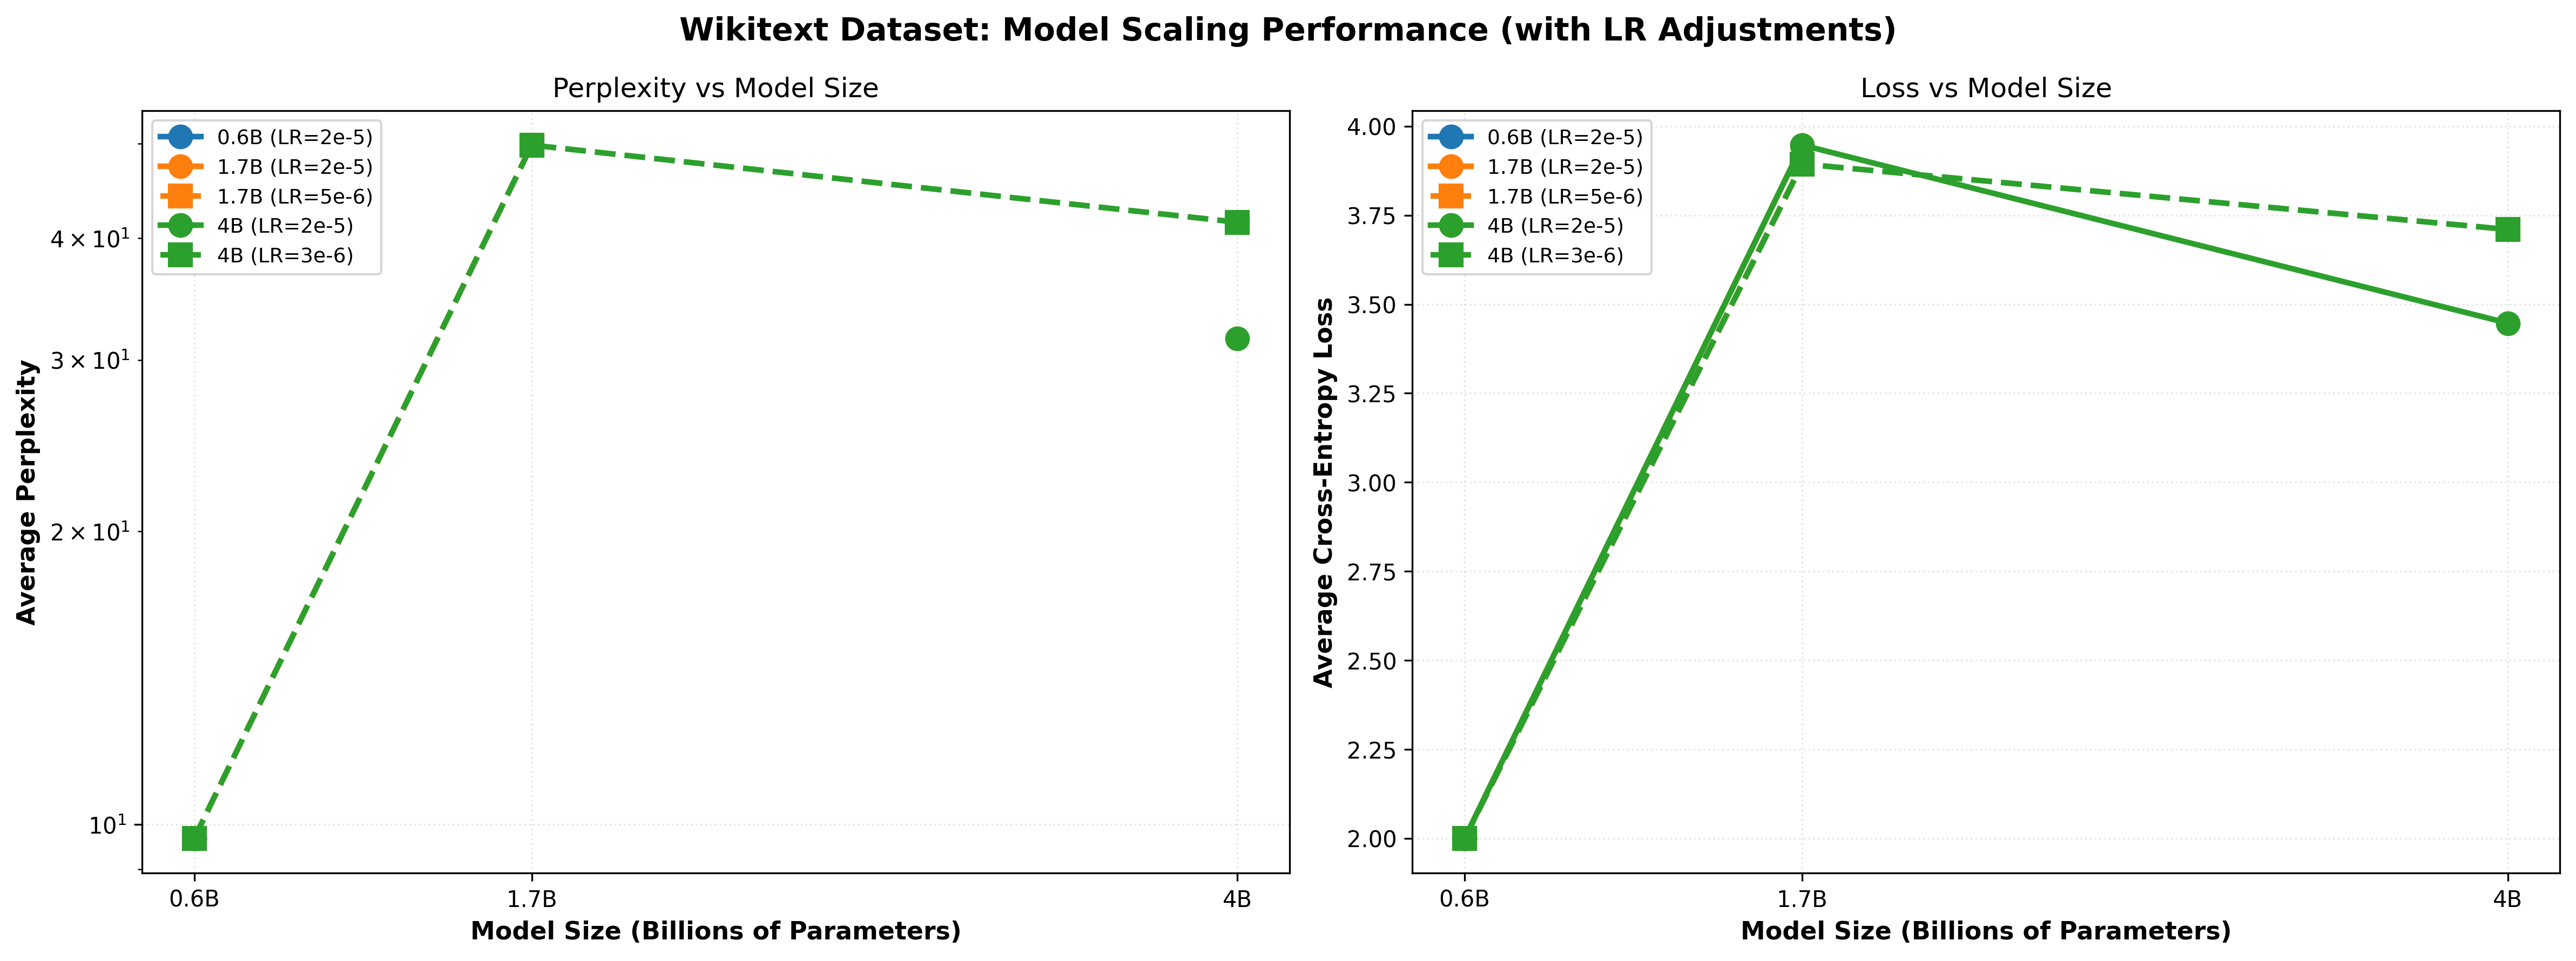
\includegraphics[width=0.9\textwidth]{figures/scaling_wikitext.png}
\caption[WikiText Dataset: Reverse Scaling]{WikiText Dataset: Severe reverse scaling phenomenon. The 1.7B model shows adjusted learning rate results (dashed line, squares) after fixing training collapse. The 4B model required 75\% LR reduction to stabilize. Clean, structured data amplifies learning rate sensitivity at larger scales.}
\label{fig:scaling_wikitext}
\end{figure}

% WikiText Dataset: Evaluation Results with LR Adjustments
% Training: WikiText (WikiText-103, 100M tokens)
% LR Adjustments: 1.7B (2e-5 → 5e-6), 4B (2e-5 → 3e-6)

\begin{table}[h]
\centering
\caption[WikiText: Learning Rate Comparison]{WikiText Dataset: Impact of Learning Rate Adjustments}
\label{tab:wikitext_lr_comparison}
\begin{tabular}{l|c|cc|cc|c|cc|cc}
\hline
\multirow{3}{*}{\textbf{Eval Dataset}} &
\multicolumn{5}{c|}{\textbf{Cross-Entropy Loss}} &
\multicolumn{5}{c}{\textbf{Perplexity}} \\
\cline{2-6} \cline{7-11}
& \textbf{0.6B} & \multicolumn{2}{c|}{\textbf{1.7B}} & \multicolumn{2}{c|}{\textbf{4B}} &
 \textbf{0.6B} & \multicolumn{2}{c|}{\textbf{1.7B}} & \multicolumn{2}{c}{\textbf{4B}} \\
\cline{3-4} \cline{5-6} \cline{8-9} \cline{10-11}
& \textbf{2e-5} & \textbf{2e-5} & \textbf{5e-6} & \textbf{2e-5} & \textbf{3e-6} &
 \textbf{2e-5} & \textbf{2e-5} & \textbf{5e-6} & \textbf{2e-5} & \textbf{3e-6} \\
\hline
 Alpaca & 2.22 & \textbf{3.24} & 3.79 & \textbf{3.48} & 3.64 & 9.23 & \textbf{25.51} & 44.22 & \textbf{32.38} & 38.06 \\
Financial News & 2.62 & \textbf{2.93} & 3.52 & 3.37 & \textbf{3.27} & 13.70 & \textbf{18.78} & 33.66 & \textbf{29.19} & \textbf{26.44} \\
 Financial QA & 3.40 & 10.67 & \textbf{4.07} & \textbf{3.37} & 3.87 & 29.90 & $\infty$ & \textbf{58.33} & \textbf{29.08} & 47.98 \\
 SEC Reports & 1.39 & \textbf{3.27} & 3.91 & \textbf{3.44} & 3.75 & 3.99 & \textbf{26.46} & 49.83 & \textbf{31.23} & 42.41 \\
 FinGPT & 1.30 & \textbf{2.11} & 4.07 & \textbf{3.57} & 3.88 & 3.67 & \textbf{8.27} & 58.55 & \textbf{35.50} & 48.30 \\
 FiQA & 2.07 & \textbf{3.14} & 3.85 & \textbf{3.53} & 3.74 & 7.89 & \textbf{23.15} & 46.81 & \textbf{34.03} & 42.04 \\
Twitter & 1.45 & \textbf{2.78} & 4.08 & \textbf{3.52} & 3.88 & 4.26 & \textbf{16.06} & 58.98 & \textbf{33.71} & 48.48 \\
\rowcolor{gray!20} \textbf{Wikitext (train)} & 1.56 & \textbf{3.42} & 3.88 & \textbf{3.30} & 3.65 & 4.78 & \textbf{30.63} & 48.44 & \textbf{27.19} & 38.60 \\
\rowcolor{blue!10} \textbf{Average} & \textbf{2.00} & \textbf{3.95} & \textbf{3.89} & \textbf{3.45} & \textbf{3.71} & \textbf{9.68} & \textbf{$\infty$} & \textbf{49.85} & \textbf{31.54} & \textbf{41.54}  \\
\hline
\end{tabular}
\end{table}


\subsection{Key Takeaway}

Comparing the three mixture strategies yields a clear hierarchy:

\textbf{1. Mixed Financial (best)}: 21.55 ppl @ 4B, 55\% spread. Optimal for financial applications. Demonstrates that \textit{in-domain diversity} (multiple financial datasets) provides better generalization than either single datasets or general-domain corpora.

\textbf{2. Mixed Wiki+Financial (moderate)}: 26.69 ppl @ 4B, 62\% spread. Acceptable when general-domain retention is explicitly required, but comes with 24\% performance cost on financial tasks.

\textbf{3. Pure WikiText (poor for finance)}: 31.54 ppl @ 4B (WikiText test set), 41.96 ppl mean financial. Excellent general-domain performance but catastrophic financial transfer. Confirms domain specialization necessity.

\textbf{Scientific Contribution}: This ranking demonstrates that \textbf{high-quality general data does not substitute for domain diversity}. In specialized domains, multiple in-domain datasets (even if individually small or noisy) outperform large, clean general corpora. This finding has implications for pretraining strategies across domains (legal, medical, scientific) beyond finance. \Cref{fig:scaling_comparison_all} visually confirms this hierarchy: the blue line (Mixed Financial) remains consistently below orange (Mixed Wiki+Financial) and green (WikiText) across all model sizes, with the performance gap widening from 0.6B to 4B.

\begin{figure}[h]
\centering
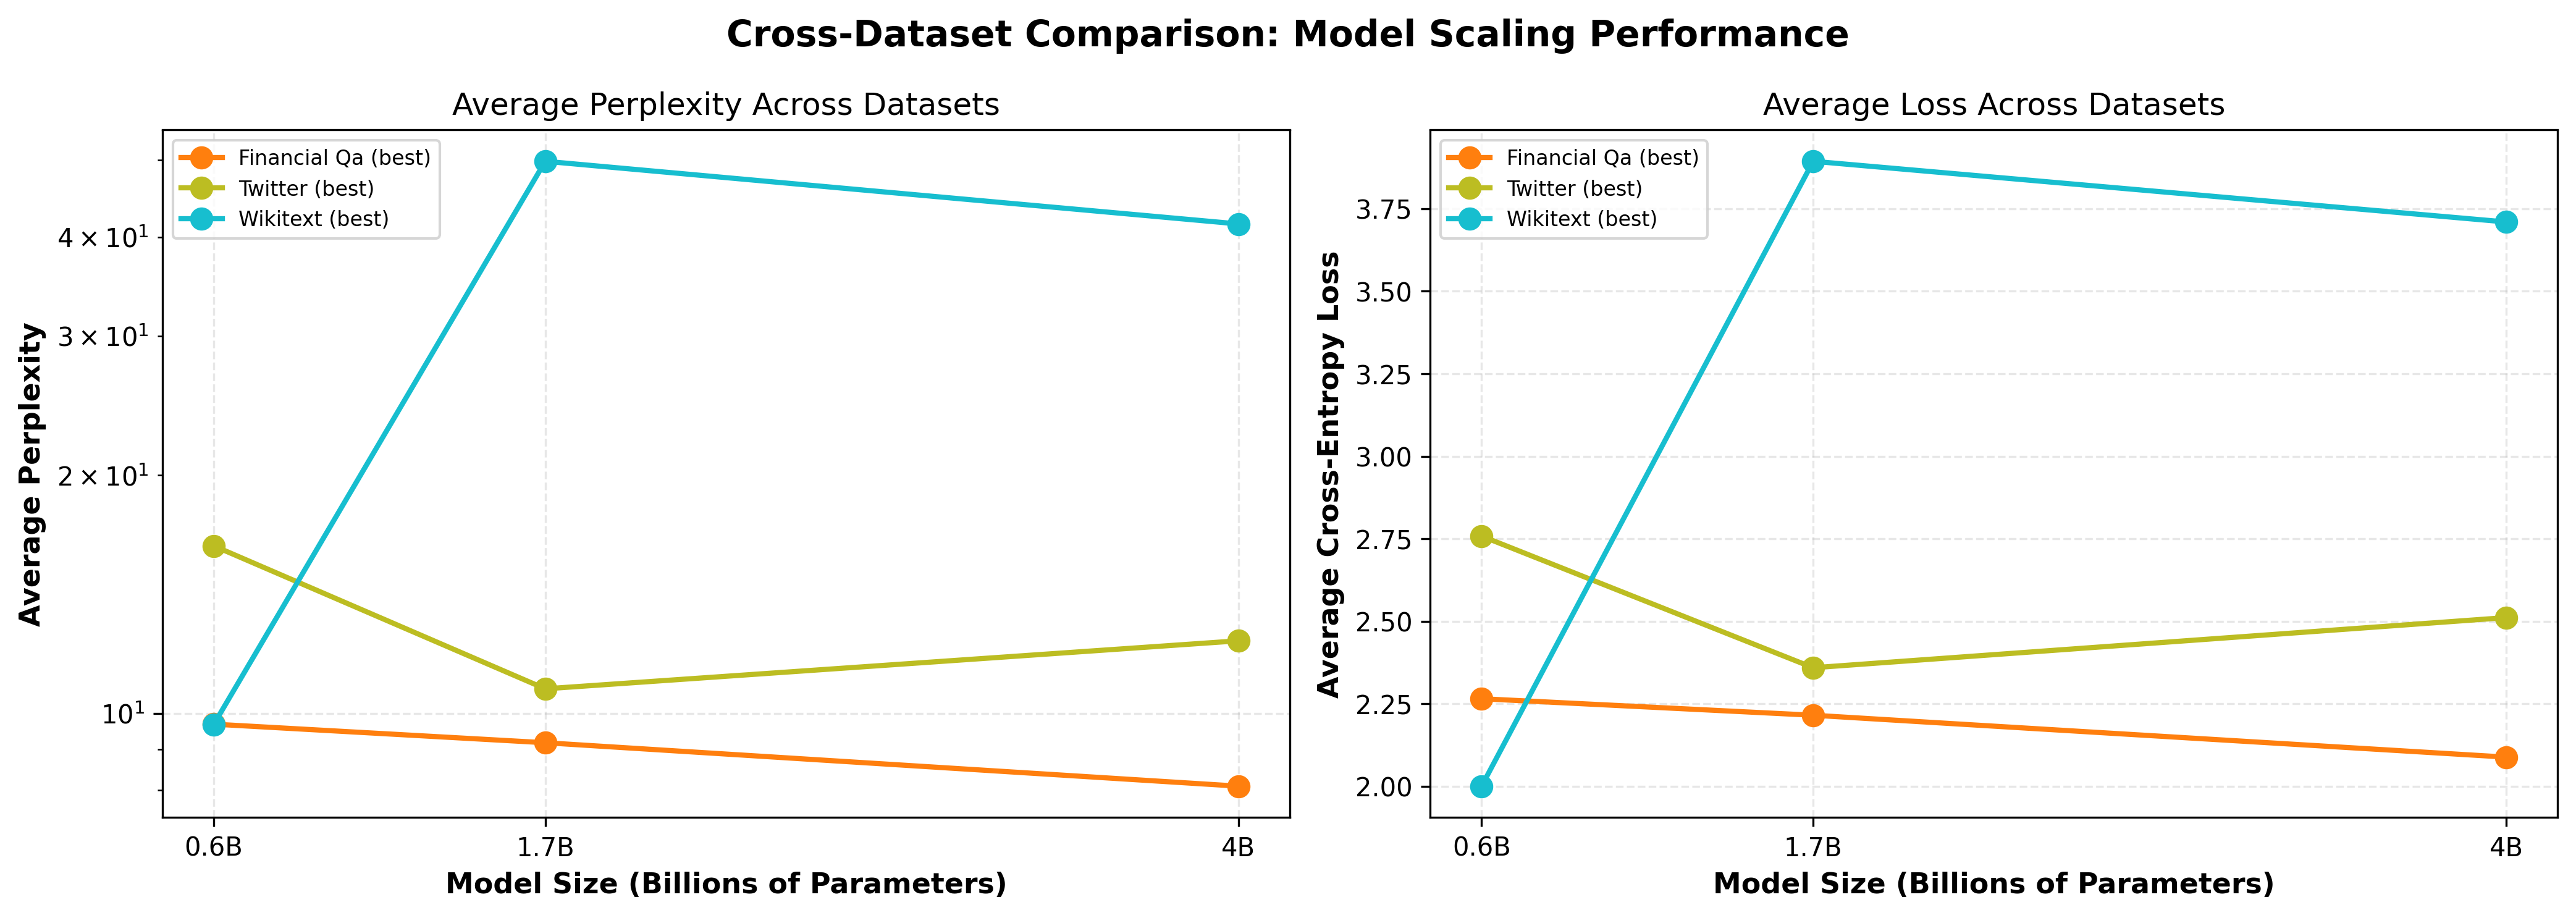
\includegraphics[width=0.9\textwidth]{figures/scaling_comparison_all.png}
\caption[Comparison of Mixture Strategies]{Comparison of all three mixture strategies across model sizes. Mixed Financial (blue) consistently outperforms Mixed Wiki+Financial (orange) and WikiText (green) on financial evaluation metrics. The divergence increases with model size, demonstrating that in-domain diversity scales better than general-domain quality.}
\label{fig:scaling_comparison_all}
\end{figure}

\section{Individual Dataset Analysis: Component Effects}

To understand which datasets contribute most to mixture performance and when standalone pretraining is viable, we trained models on each of the 7 financial datasets individually. Results reveal a clear relationship between dataset size and pretraining viability.

\subsection{Large Datasets}

Two datasets exceed 80M tokens: News Articles (197M) and SEC Reports (80M). Both demonstrate viable standalone pretraining with reasonable generalization.

\textbf{News Articles (Lettria, 197M tokens)}:
\begin{itemize}
\item \textbf{Training}: 2-3 epochs across model sizes, minimal overtraining
\item \textbf{Performance}: 0.6B: 52.25 ppl, 1.7B: 22.91 ppl, 4B: 17.47 ppl (News test set)
\item \textbf{Normal scaling}: Consistent improvements with model size (56\% 0.6B→1.7B, 24\% 1.7B→4B)
\item \textbf{Cross-dataset generalization}: Strong transfer to SEC (33.46 ppl) and Alpaca (29.75 ppl), moderate to FiQA (31.69 ppl) and FinGPT (38.03 ppl), poor to Twitter (38.98 ppl) and Financial QA (38.90 ppl)
\item \textbf{Relative spread}: 65.53\% (4B model), among the lowest for individual datasets, indicating consistent generalization
\end{itemize}

\textbf{SEC Reports (80M tokens)}:
\begin{itemize}
\item \textbf{Training}: 24 epochs (varies by model size), moderate overtraining
\item \textbf{Performance}: 0.6B: 41.12 ppl, 1.7B: 19.36 ppl, 4B: 15.91 ppl (SEC test set)
\item \textbf{Normal scaling}: Expected improvements at all scales
\item \textbf{Cross-dataset generalization}: Strong transfer to News (16.67 ppl, similar document length), moderate to FinGPT (18.68 ppl) and Alpaca (18.54 ppl), weaker to short-form tasks (FiQA 19.34 ppl, Twitter 18.12 ppl, Financial QA 17.39 ppl)
\item \textbf{Relative spread}: 19.32\% (4B model), lowest among all experiments on SEC test set itself, but 19.32\% across all 8 evaluation sets
\end{itemize}

\textbf{Long-Form Transfer Pattern}: Both News and SEC models transfer well to each other (correlation: 0.82), suggesting that document length and narrative structure drive transferability. Models pretrained on long-form content struggle with short-form social media (Twitter) and conversational Q\&A formats.

\textbf{Viability Conclusion}: Datasets exceeding 80-100M tokens support standalone pretraining with acceptable generalization, particularly within similar document formats. For specialized applications (e.g., SEC filing analysis), single large datasets may suffice. \Cref{fig:scaling_news_articles,fig:scaling_sec_reports} demonstrate clean scaling curves with no reverse scaling or training instabilities, confirming that large dataset size provides sufficient training signal for stable optimization across model scales.

\begin{figure}[h]
\centering
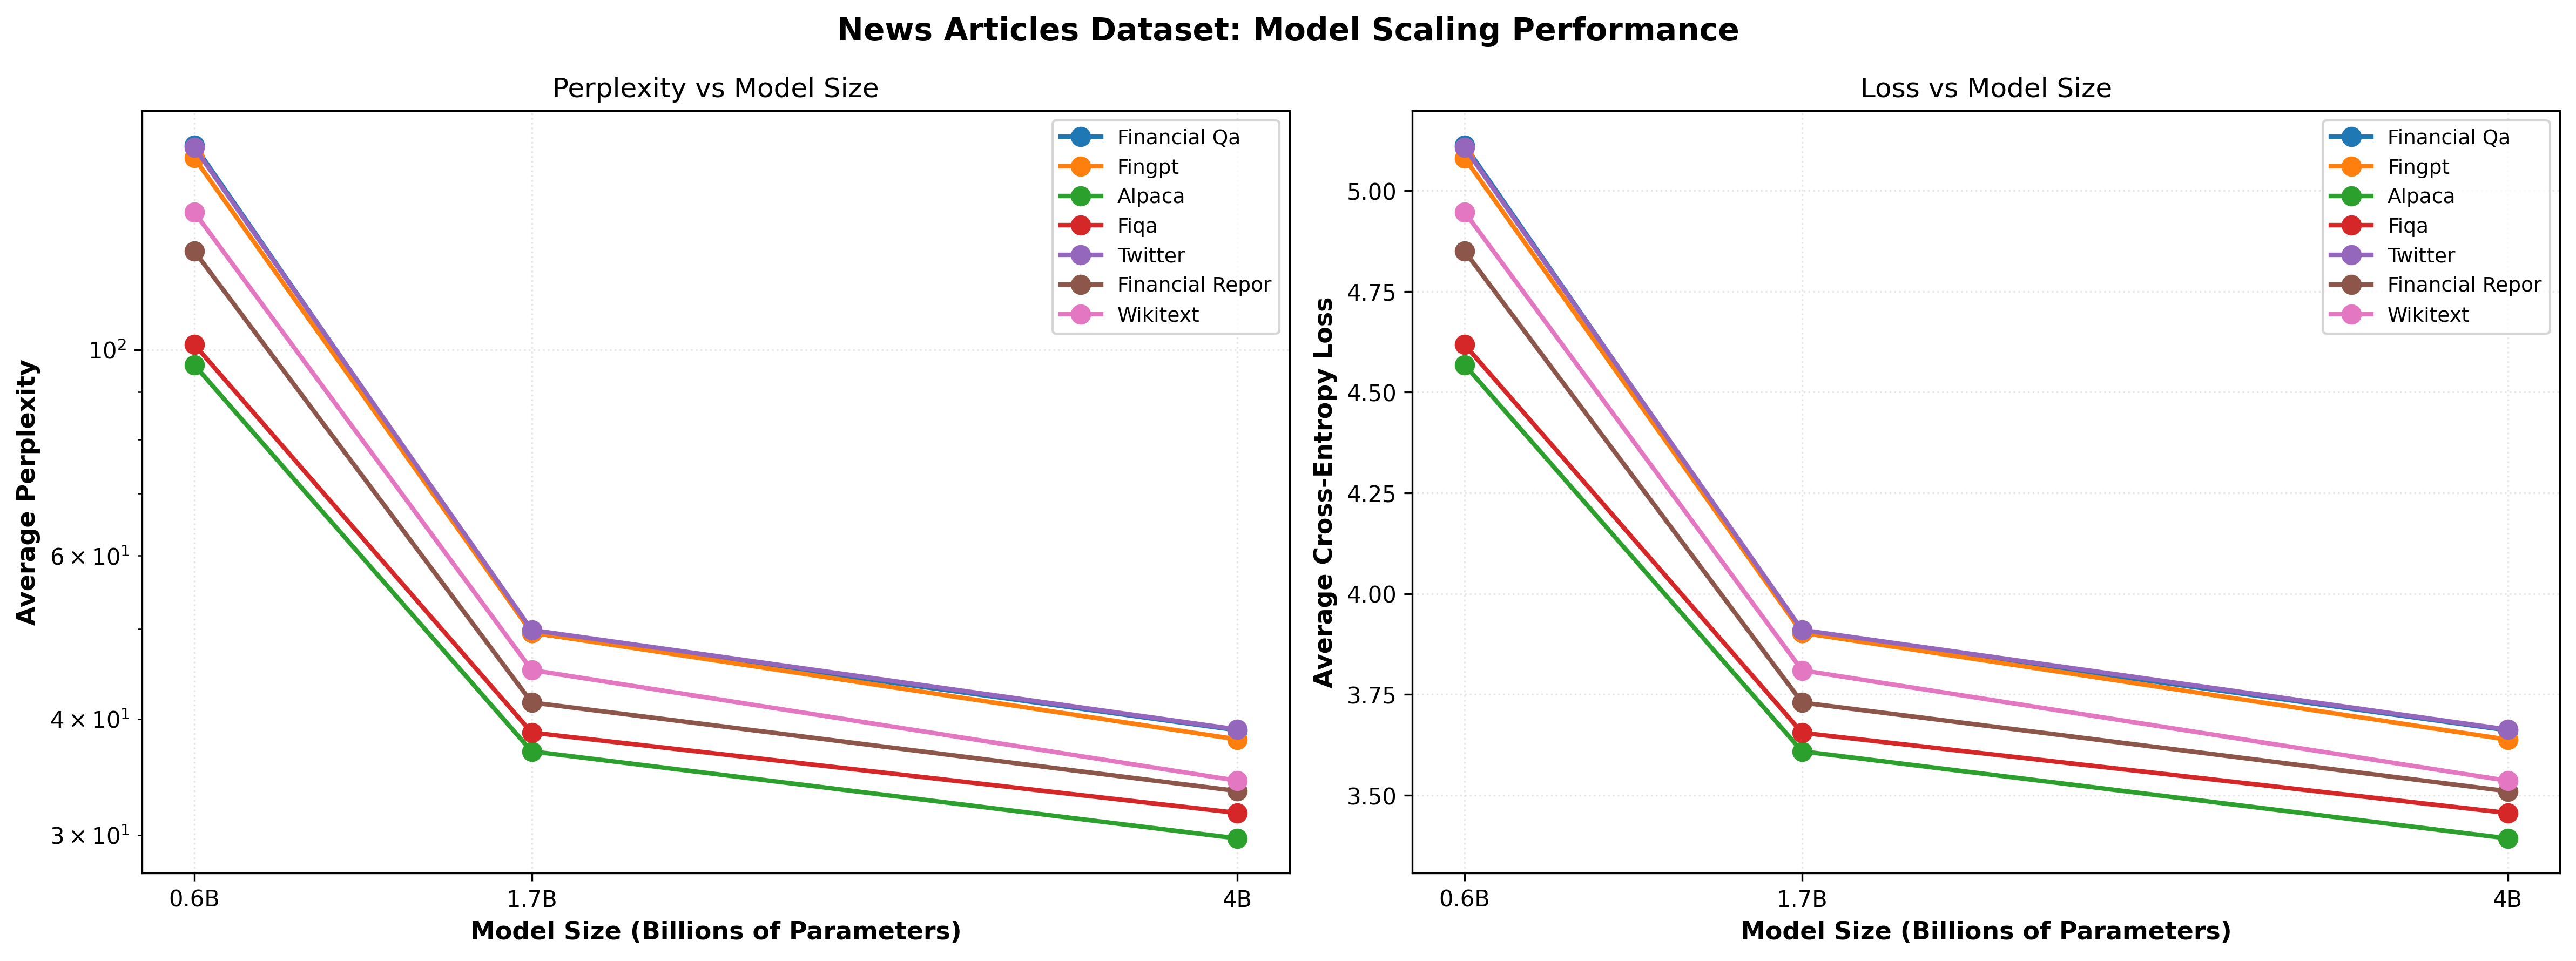
\includegraphics[width=0.9\textwidth]{figures/scaling_news_articles.png}
\caption[Financial News Dataset: Scaling Behavior]{Financial News Articles Dataset: Excellent normal scaling with 66.6\% total improvement (0.6B to 4B). Large dataset size (197M tokens) provides sufficient diversity for stable training across all model sizes with minimal overtraining (2-3 epochs).}
\label{fig:scaling_news_articles}
\end{figure}

\begin{figure}[h]
\centering
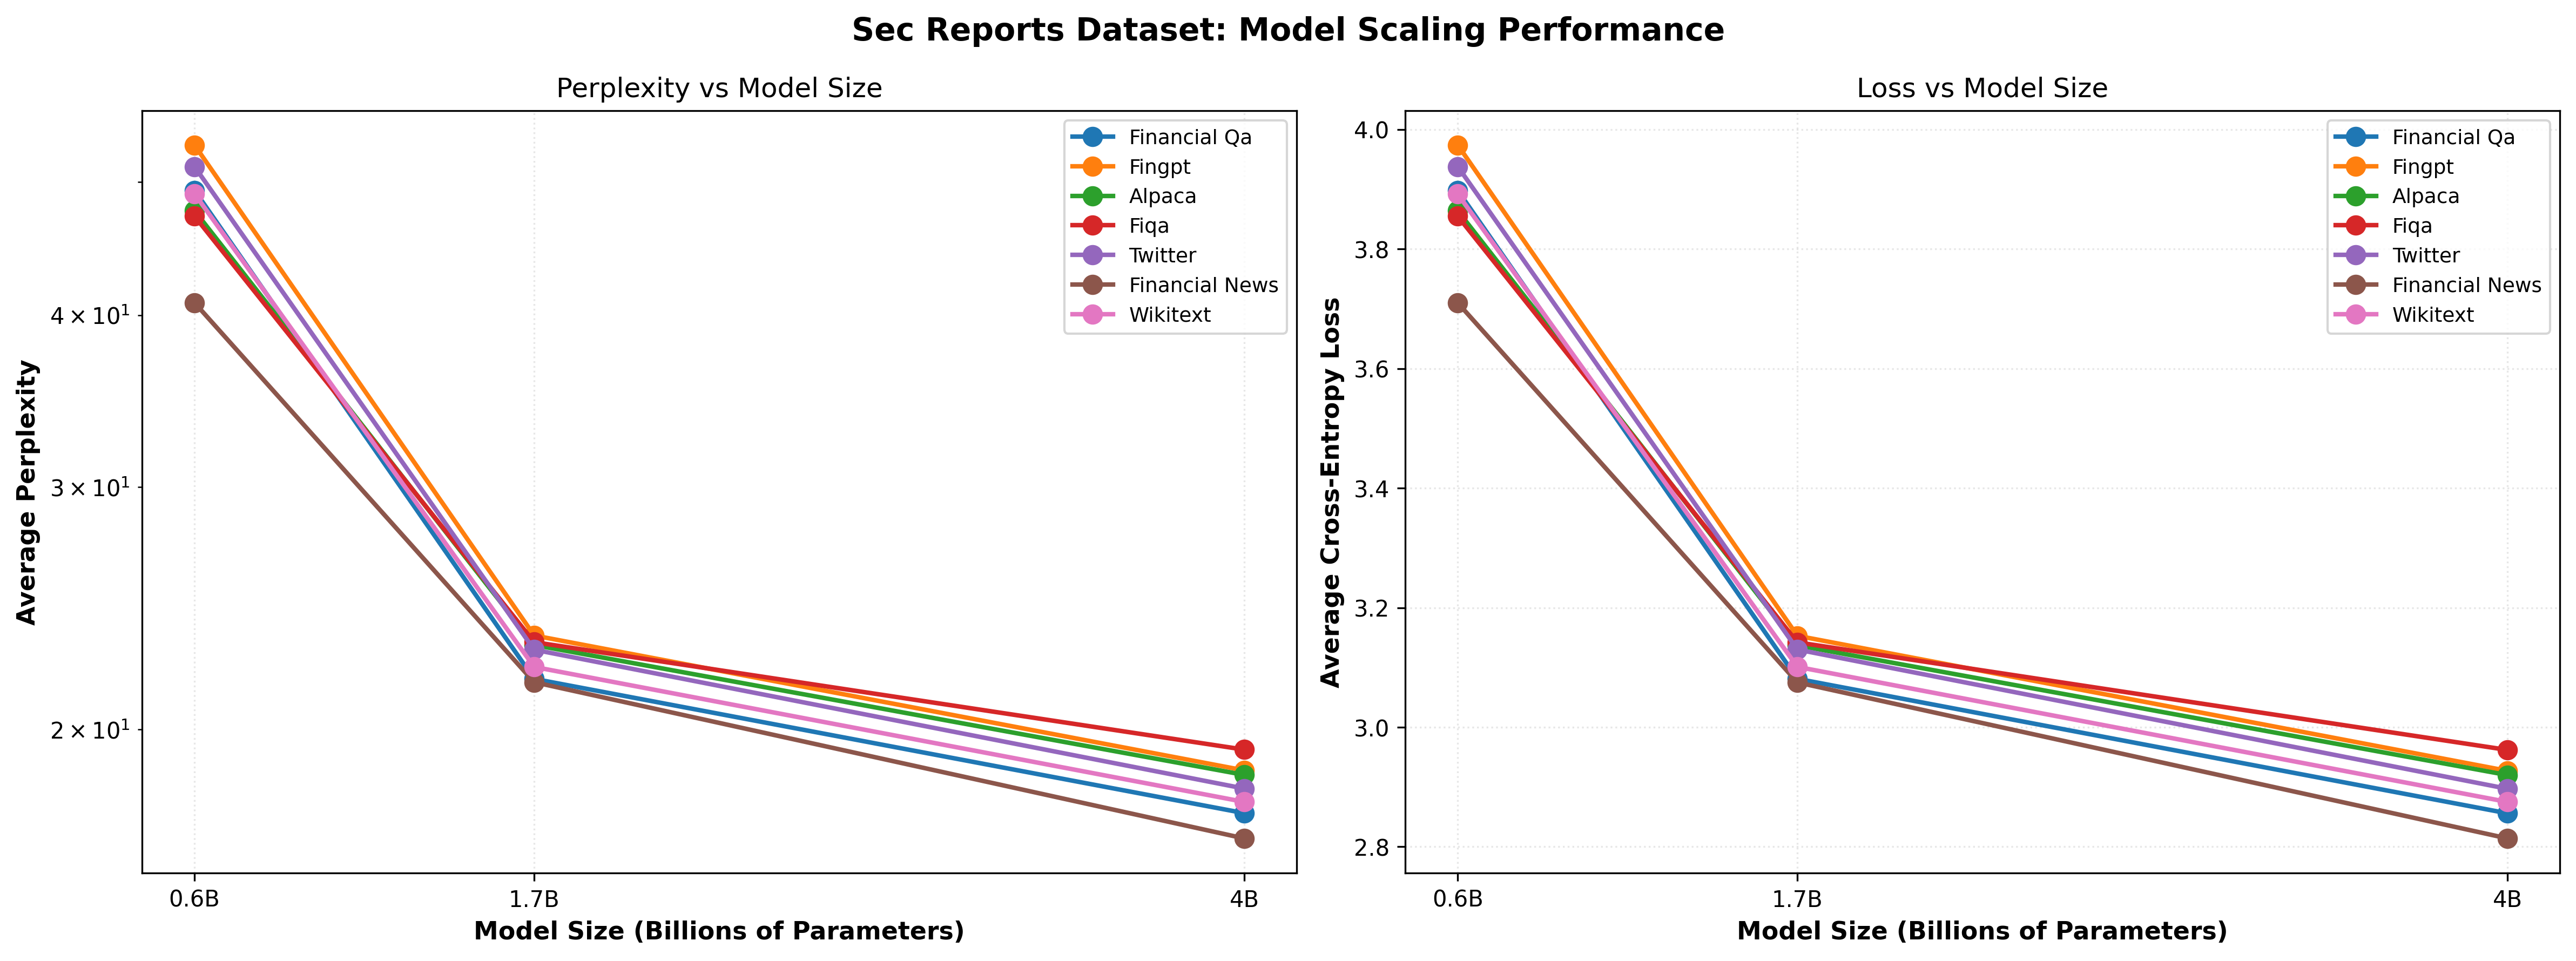
\includegraphics[width=0.9\textwidth]{figures/scaling_sec_reports.png}
\caption[SEC Reports Dataset: Scaling Behavior]{SEC Reports Dataset: Consistent normal scaling with 61.3\% total improvement. The 80M token corpus supports standalone pretraining with moderate overtraining (24 epochs). Strong transfer to similar long-form documents.}
\label{fig:scaling_sec_reports}
\end{figure}

% Financial News Dataset: Evaluation Results
% Training: Financial News (Financial news articles, 194.47M tokens)
% All models trained with LR=2e-5

\begin{table}[htbp]
\centering
\caption[Financial News: Evaluation Results]{Financial News Dataset: Evaluation Across Multiple Datasets}
\label{tab:news_articles_results}
\begin{tabular}{l|ccc|ccc}
\hline
\textbf{Eval Dataset} & \multicolumn{3}{c|}{\textbf{Cross-Entropy Loss}} & \multicolumn{3}{c}{\textbf{Perplexity}} \\
\cline{2-4} \cline{5-7}
  & \textbf{0.6B} & \textbf{1.7B} & \textbf{4B} & \textbf{0.6B} & \textbf{1.7B} & \textbf{4B} \\
\hline
Alpaca & 4.57 & 3.61 & \textbf{3.39} & 96.31 & \textbf{36.92} & \textbf{29.75} \\
\textbf{Financial News} & \textbf{3.96} & \textbf{3.13} & \textbf{2.86} & \textbf{52.25} & \textbf{22.91} & \textbf{17.47} \\
Financial QA & 5.11 & 3.90 & \textbf{3.66} & 166.1 & \textbf{49.53} & \textbf{38.90} \\
SEC Reports & 4.85 & 3.73 & \textbf{3.51} & 127.7 & \textbf{41.68} & \textbf{33.46} \\
FinGPT & 5.08 & 3.90 & \textbf{3.64} & 160.9 & \textbf{49.56} & \textbf{38.03} \\
FiQA & 4.62 & 3.65 & \textbf{3.46} & 101.3 & \textbf{38.68} & \textbf{31.69} \\
Twitter & 5.11 & 3.91 & \textbf{3.66} & 165.2 & \textbf{49.88} & \textbf{38.98} \\
Wikitext & 4.95 & 3.81 & \textbf{3.54} & 140.7 & \textbf{45.17} & \textbf{34.33} \\
\hline
\textbf{Average} & \textbf{4.78} & \textbf{3.71} & \textbf{3.47} & \textbf{126.3} & \textbf{41.79} & \textbf{32.82} \\
\hline
\end{tabular}
\end{table}


% SEC Reports Dataset: Evaluation Results
% Training: SEC Reports (SEC 10-K/10-Q filings, 80M tokens)
% All models trained with LR=2e-5

\begin{table}[h]
\centering
\caption[SEC Reports: Evaluation Results]{SEC Reports Dataset: Evaluation Across Multiple Datasets}
\label{tab:sec_reports_results}
\begin{tabular}{l|ccc|ccc}
\hline
\textbf{Eval Dataset} & \multicolumn{3}{c|}{\textbf{Cross-Entropy Loss}} & \multicolumn{3}{c}{\textbf{Perplexity}} \\
\cline{2-4} \cline{5-7}
  & \textbf{0.6B} & \textbf{1.7B} & \textbf{4B} & \textbf{0.6B} & \textbf{1.7B} & \textbf{4B} \\
Alpaca & 3.86 & 3.14 & \textbf{2.92} & 47.65 & \textbf{23.04} & \textbf{18.54} \\
Financial News & 3.71 & 3.08 & \textbf{2.81} & 40.85 & \textbf{21.65} & \textbf{16.67} \\
Financial Qa & 3.90 & 3.08 & \textbf{2.86} & 49.30 & \textbf{21.77} & \textbf{17.39} \\
Fingpt & 3.97 & 3.15 & \textbf{2.93} & 53.18 & \textbf{23.41} & \textbf{18.68} \\
Fiqa & 3.85 & 3.14 & \textbf{2.96} & 47.22 & \textbf{23.15} & \textbf{19.34} \\
Twitter & 3.94 & 3.13 & \textbf{2.90} & 51.30 & \textbf{22.86} & \textbf{18.12} \\
Wikitext & 3.89 & 3.10 & \textbf{2.88} & 49.02 & \textbf{22.21} & \textbf{17.72} \\
\hline
\end{tabular}
\end{table}



\subsection{Medium Datasets}

Three datasets range from 4-19M tokens: FinGPT Sentiment (19M), Finance Alpaca (17M), FiQA (4M). These show moderate overtraining and task-specific strengths.

\textbf{FinGPT Sentiment (19M tokens)}:
\begin{itemize}
\item \textbf{Training}: 30 epochs, noticeable overtraining on smallest model
\item \textbf{Performance}: 0.6B: 32.78 ppl, 1.7B: 9.56 ppl, 4B: 5.67 ppl (FinGPT test set)
\item \textbf{Instruction-following strength}: Strong transfer to Alpaca (8.27 ppl) and FiQA (8.16 ppl), both instruction-formatted datasets. Weaker on document datasets (News 7.92 ppl, SEC 6.20 ppl)
\item \textbf{Relative spread}: 37.07\% (4B model), moderate variance indicating task-type specialization
\end{itemize}

\textbf{Finance Alpaca (17M tokens)}:
\begin{itemize}
\item \textbf{Training}: 12 epochs, moderate overtraining
\item \textbf{Performance}: 0.6B: 63.73 ppl, 1.7B: 15.61 ppl, 4B: 8.22 ppl (Alpaca test set)
\item \textbf{Educational Q\&A focus}: Best transfer to FiQA (9.22 ppl) and FinGPT (9.18 ppl). Poor on documents (News 8.58 ppl, SEC 8.25 ppl) and Twitter (8.97 ppl)
\item \textbf{Relative spread}: 11.51\% (4B model), higher variance reflects narrow task focus
\end{itemize}

\textbf{FiQA (4M tokens)}:
\begin{itemize}
\item \textbf{Training}: 7 epochs (normalized by short examples), approaching overtraining threshold
\item \textbf{Performance}: 0.6B: 64.75 ppl, 1.7B: 12.99 ppl, 4B: 7.08 ppl (FiQA test set)
\item \textbf{Conversational Q\&A specialization}: Excellent on FiQA itself, good on Alpaca (7.12 ppl) and FinGPT (7.01 ppl), poor on long-form (News 7.43 ppl, SEC 6.14 ppl)
\item \textbf{Relative spread}: 18.97\% (4B model)
\end{itemize}

\textbf{Medium Dataset Conclusion}: Datasets in the 4-20M token range support pretraining but exhibit task-type specialization. Instruction-formatted datasets (FinGPT, Alpaca, FiQA) transfer well to each other but poorly to document formats. For general financial applications, these datasets should be mixed rather than used standalone. As shown in \Cref{fig:scaling_fingpt,fig:scaling_alpaca,fig:scaling_fiqa}, all three medium datasets maintain normal scaling patterns despite moderate overtraining (12-30 epochs), with smooth perplexity reduction curves and no optimization instabilities. Detailed cross-dataset performance in \Cref{tab:fingpt_results,tab:alpaca_results,tab:fiqa_results} confirms task-type clustering: strong mutual transfer within instruction-formatted tasks, weak transfer to document formats.

\begin{figure}[h]
\centering
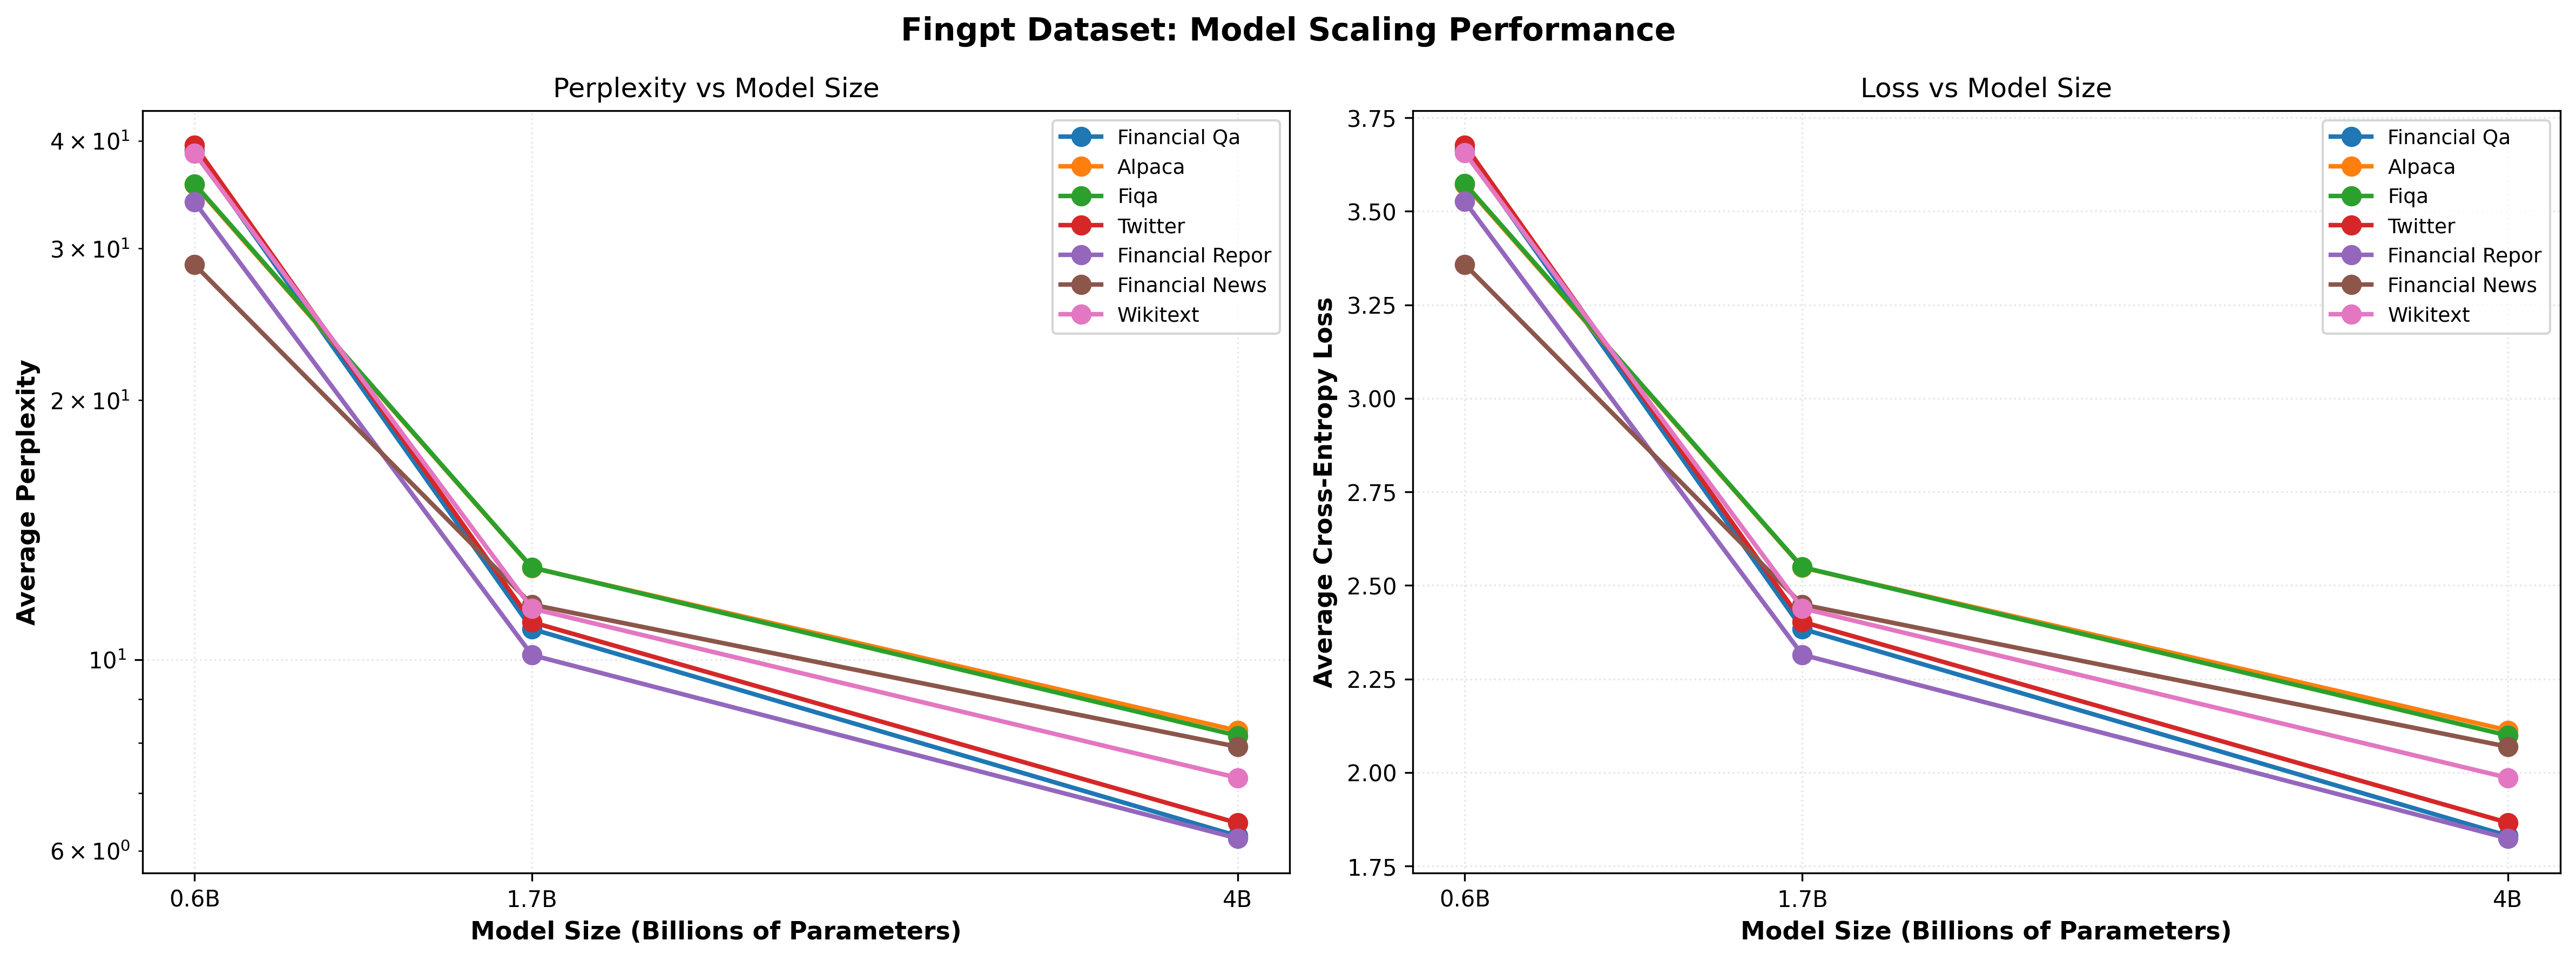
\includegraphics[width=0.9\textwidth]{figures/scaling_fingpt.png}
\caption[FinGPT Sentiment Dataset: Scaling Behavior]{FinGPT Sentiment Dataset: Normal scaling with 82.7\% improvement despite moderate overtraining (30 epochs). Instruction-following format benefits from increased model capacity, showing strong transfer to similar task types.}
\label{fig:scaling_fingpt}
\end{figure}

\begin{figure}[h]
\centering
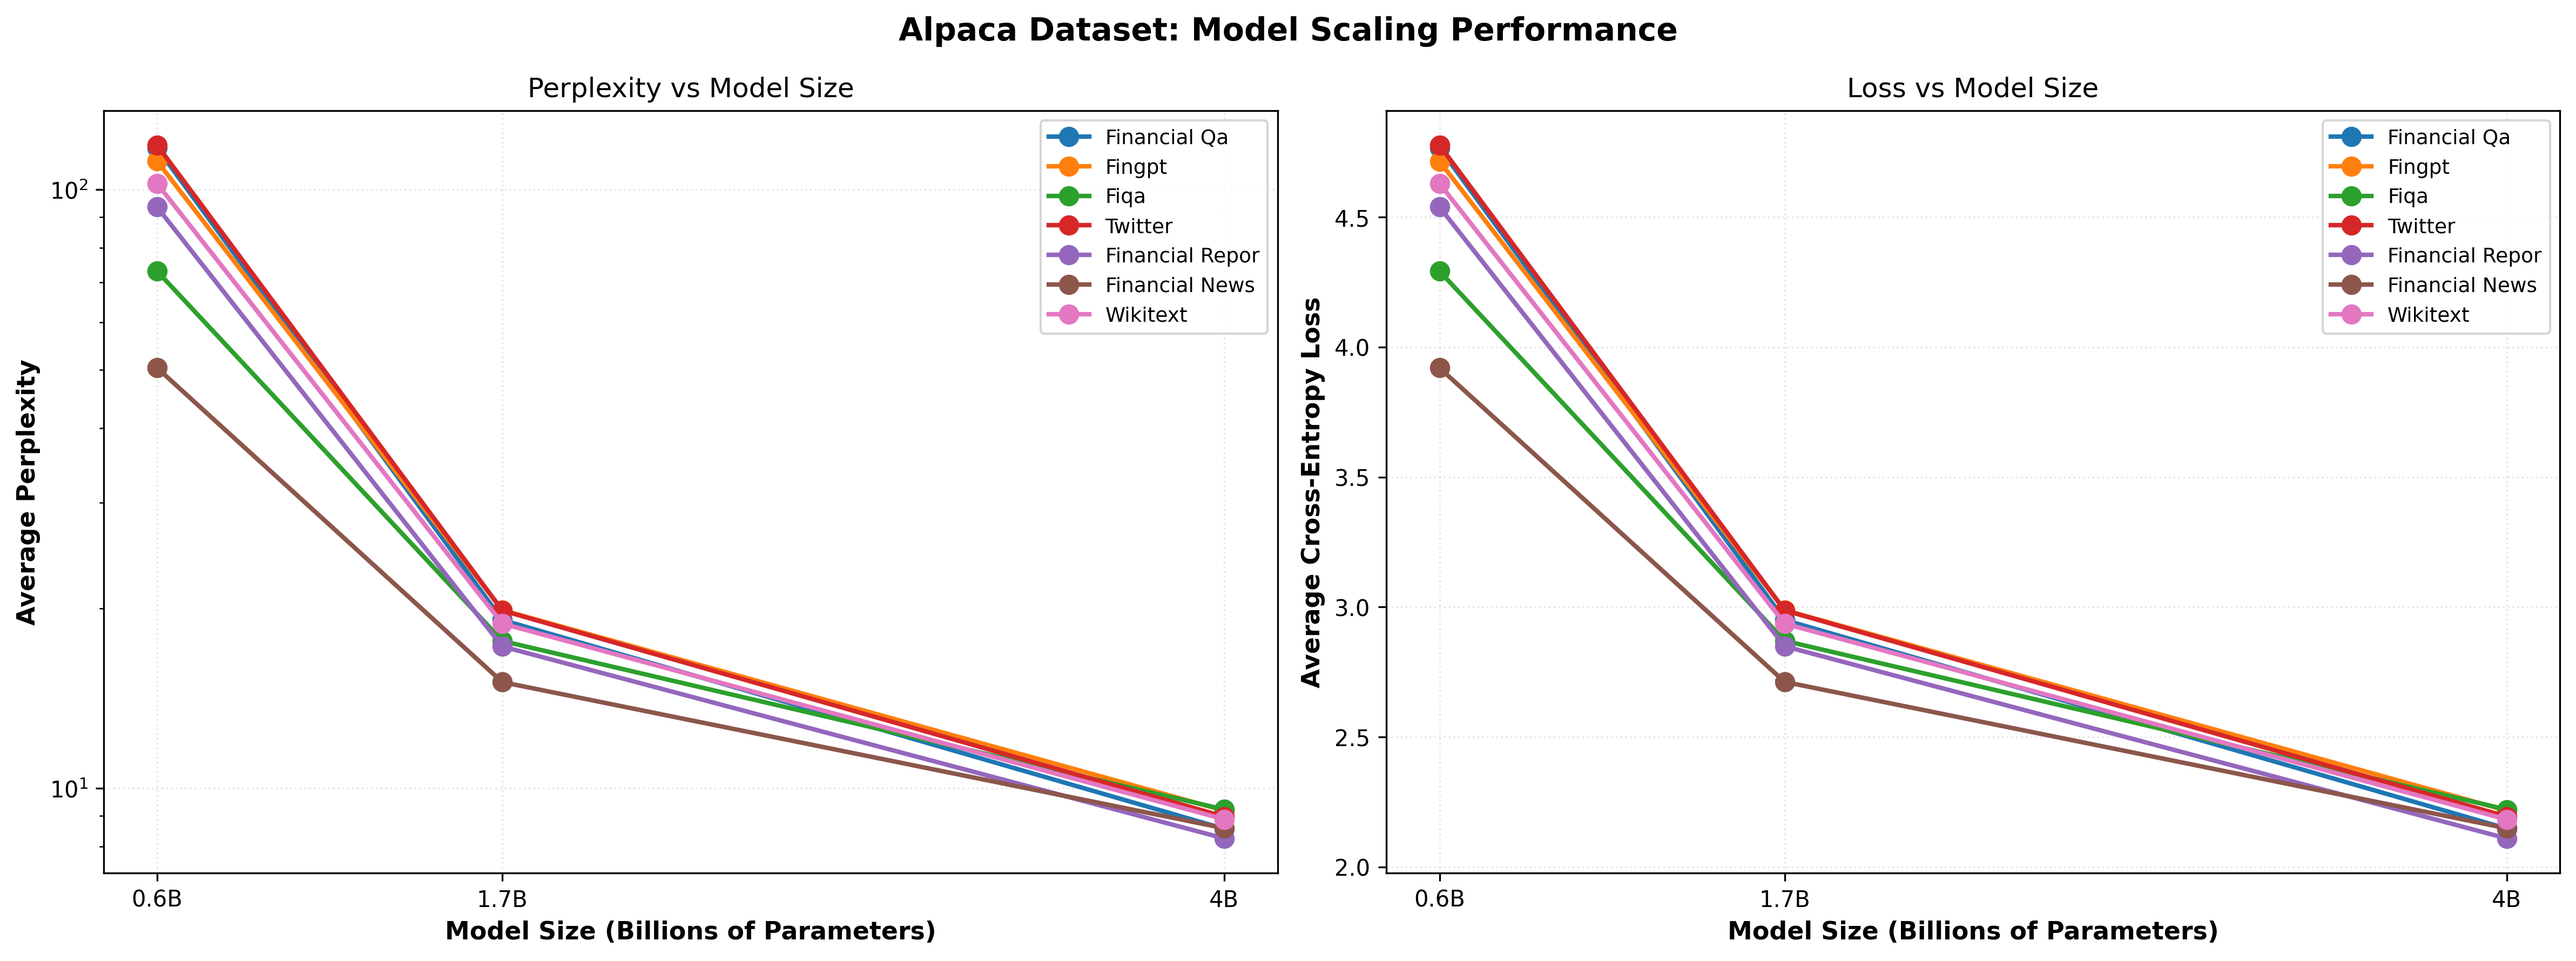
\includegraphics[width=0.9\textwidth]{figures/scaling_alpaca.png}
\caption[Finance Alpaca Dataset: Scaling Behavior]{Finance Alpaca Dataset: Consistent 87.1\% improvement across model sizes. Educational Q\&A format shows reliable scaling despite 12 epochs of training, but exhibits narrow task focus with 11.51\% cross-dataset variance.}
\label{fig:scaling_alpaca}
\end{figure}

\begin{figure}[h]
\centering
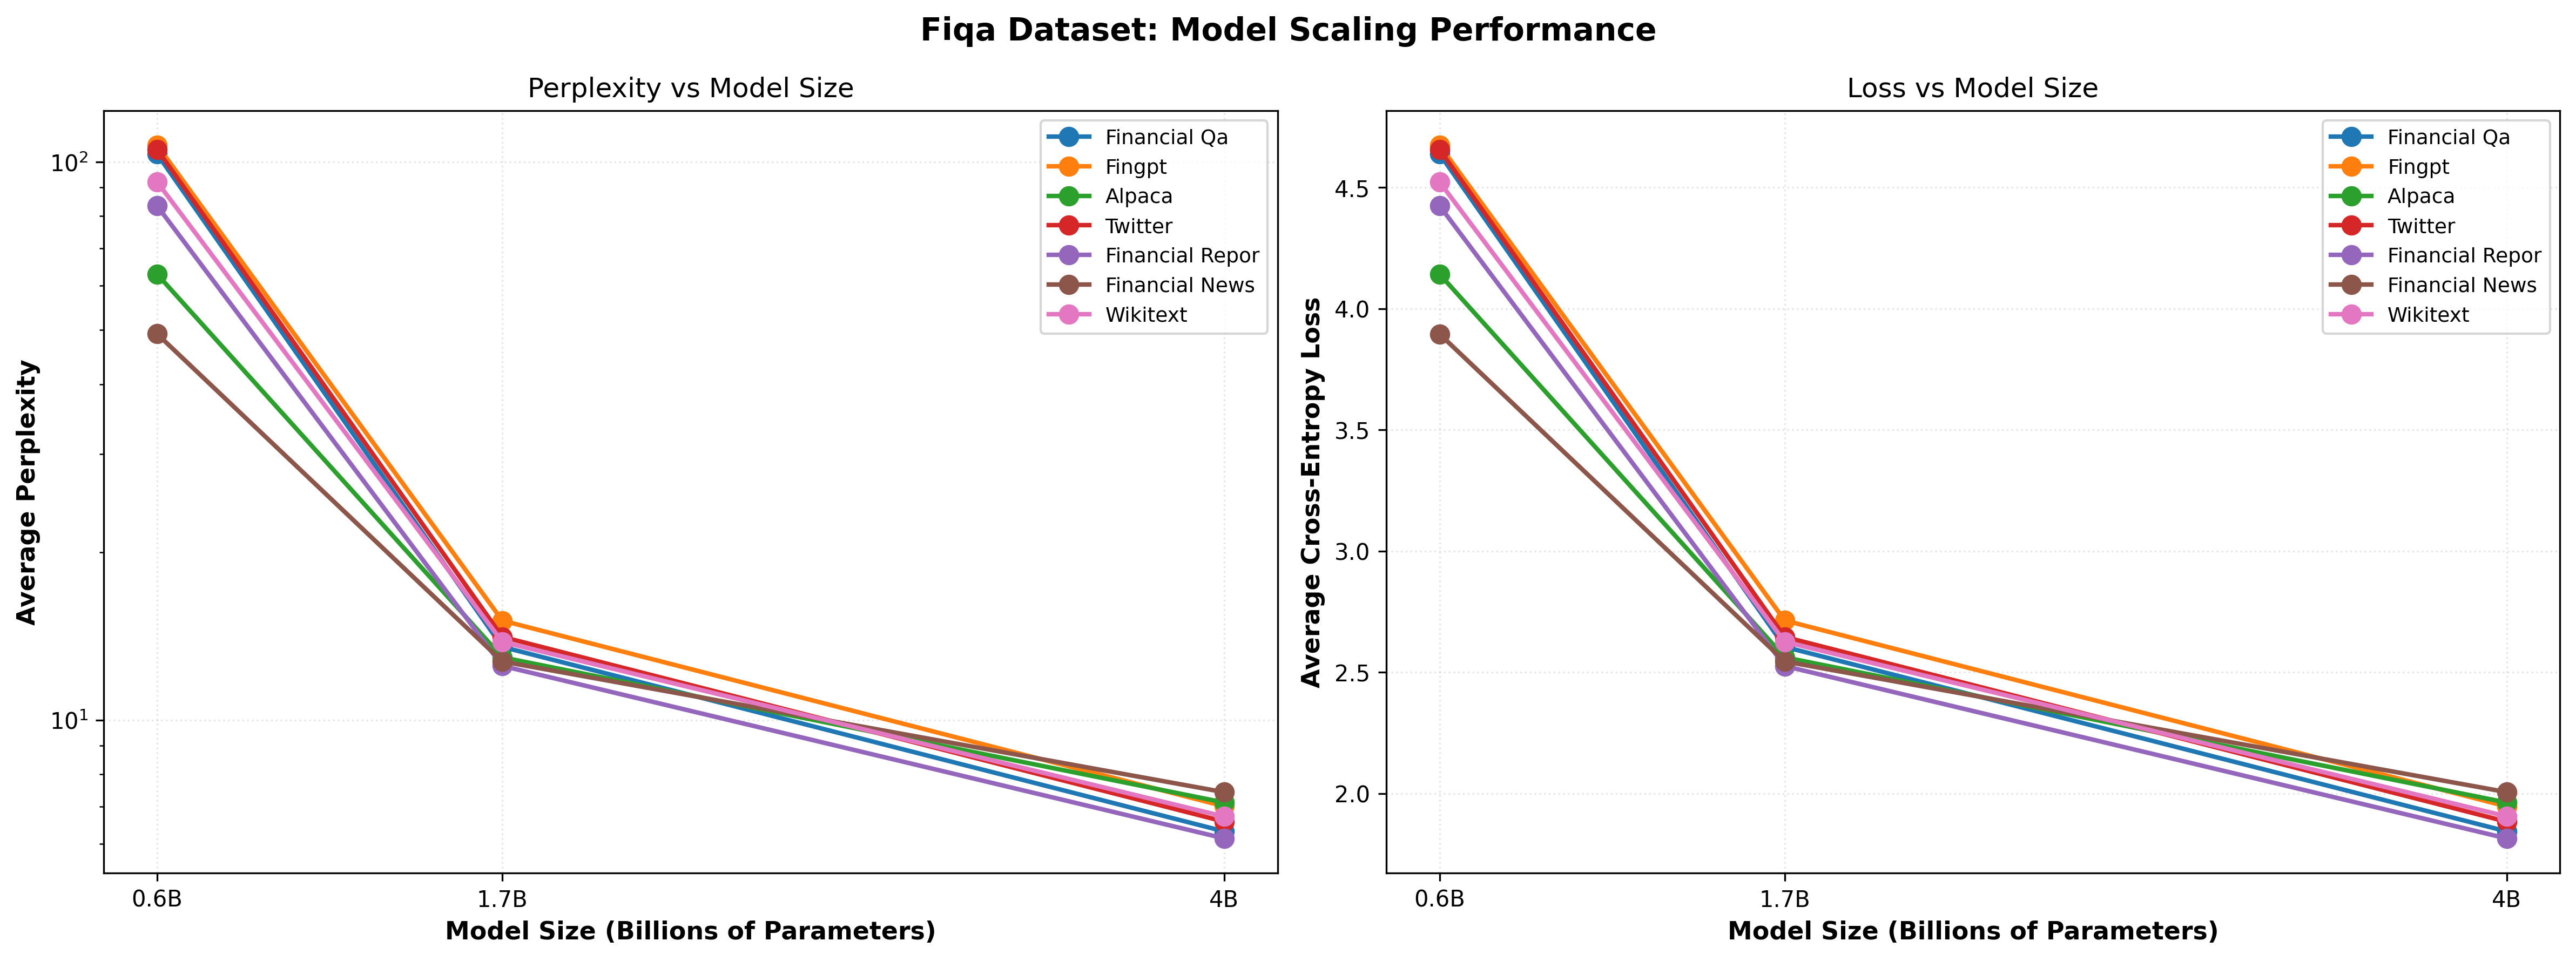
\includegraphics[width=0.9\textwidth]{figures/scaling_fiqa.png}
\caption[FiQA Dataset: Scaling Behavior]{FiQA Dataset: Strong normal scaling with 89.1\% total improvement. Despite small size (4M tokens), conversational Q\&A format produces stable training and excellent in-domain performance, though with high variance (18.97\%) on out-of-format tasks.}
\label{fig:scaling_fiqa}
\end{figure}

% FinGPT Sentiment Dataset: Evaluation Results
% Training: FinGPT Sentiment (FinGPT/fingpt-sentiment-train, 19M tokens)
% All models trained with LR=2e-5

\begin{table}[h]
\centering
\caption{FinGPT Sentiment Dataset: Evaluation Across Multiple Datasets}
\label{tab:fingpt_results}
\begin{tabular}{l|ccc|ccc}
\hline
\textbf{Eval Dataset} & \multicolumn{3}{c|}{\textbf{Cross-Entropy Loss}} & \multicolumn{3}{c}{\textbf{Perplexity}} \\n\cline{2-4} \cline{5-7}
  & \textbf{0.6B} & \textbf{1.7B} & \textbf{4B} & \textbf{0.6B} & \textbf{1.7B} & \textbf{4B} \\
Alpaca & 3.57 & 2.55 & \textbf{2.11} & 35.55 & \textbf{12.78} & \textbf{8.27} \
 Financial News & 3.36 & 2.45 & \textbf{2.07} & 28.72 & \textbf{11.58} & \textbf{7.92} \
 Financial Qa & 3.66 & 2.38 & \textbf{1.83} & 38.96 & \textbf{10.85} & \textbf{6.24} \
 Financial Repor & 3.53 & 2.31 & \textbf{1.82} & 33.97 & \textbf{10.12} & \textbf{6.20} \
 Fiqa & 3.57 & 2.55 & \textbf{2.10} & 35.64 & \textbf{12.79} & \textbf{8.16} \
 Twitter & 3.68 & 2.40 & \textbf{1.87} & 39.54 & \textbf{11.05} & \textbf{6.46} \
 Wikitext & 3.66 & 2.44 & \textbf{1.99} & 38.70 & \textbf{11.46} & \textbf{7.29} \
\hline
\end{tabular}
\end{table}



% Finance Alpaca Dataset: Evaluation Results
% Training: Finance Alpaca (gbharti/finance-alpaca, 8.46M tokens)
% All models trained with LR=2e-5

\begin{table}[h]
\centering
\caption[Finance Alpaca: Evaluation Results]{Finance Alpaca Dataset: Evaluation Across Multiple Datasets}
\label{tab:alpaca_results}
\begin{tabular}{l|ccc|ccc}
\hline
\textbf{Eval Dataset} & \multicolumn{3}{c|}{\textbf{Cross-Entropy Loss}} & \multicolumn{3}{c}{\textbf{Perplexity}} \\
\cline{2-4} \cline{5-7}
  & \textbf{0.6B} & \textbf{1.7B} & \textbf{4B} & \textbf{0.6B} & \textbf{1.7B} & \textbf{4B} \\
\textbf{Alpaca} & \textbf{4.15} & \textbf{2.75} & \textbf{2.11} & \textbf{63.73} & \textbf{15.61} & \textbf{8.22} \\
Financial News & 3.92 & 2.71 & 2.15 & 50.40 & 15.05 & 8.58 \\
Financial QA & 4.77 & 2.95 & 2.15 & 117.4 & 19.11 & 8.56 \\
SEC Reports & 4.54 & 2.85 & 2.11 & 93.56 & 17.26 & 8.25 \\
FinGPT & 4.71 & 2.99 & 2.22 & 111.7 & 19.85 & 9.18 \\
FiQA & 4.29 & 2.87 & 2.22 & 73.12 & 17.63 & 9.22 \\
Twitter & 4.78 & 2.99 & 2.19 & 118.7 & 19.82 & 8.97 \\
Wikitext & 4.63 & 2.94 & 2.18 & 102.4 & 18.85 & 8.88 \\
\hline
\textbf{Average} & \textbf{4.47} & \textbf{2.88} & \textbf{2.17} & \textbf{91.37} & \textbf{17.90} & \textbf{8.73} \\
\hline
\end{tabular}
\end{table}


% FiQA Dataset: Evaluation Results
% Training: FiQA (FiQA dataset, 4M tokens)
% All models trained with LR=2e-5

\begin{table}[h]
\centering
\caption[FiQA: Evaluation Results]{FiQA Dataset: Evaluation Across Multiple Datasets}
\label{tab:fiqa_results}
\begin{tabular}{l|ccc|ccc}
\hline
\textbf{Eval Dataset} & \multicolumn{3}{c|}{\textbf{Cross-Entropy Loss}} & \multicolumn{3}{c}{\textbf{Perplexity}} \\
\cline{2-4} \cline{5-7}
  & \textbf{0.6B} & \textbf{1.7B} & \textbf{4B} & \textbf{0.6B} & \textbf{1.7B} & \textbf{4B} \\
Alpaca & 4.14 & 2.56 & \textbf{1.96} & 62.97 & \textbf{12.96} & \textbf{7.12} \\
Financial News & 3.90 & 2.54 & \textbf{2.01} & 49.22 & \textbf{12.74} & \textbf{7.43} \\
Financial Qa & 4.64 & 2.60 & \textbf{1.84} & 103.4 & \textbf{13.53} & \textbf{6.32} \\
Financial Repor & 4.42 & 2.53 & \textbf{1.81} & 83.48 & \textbf{12.51} & \textbf{6.14} \\
Fingpt & 4.67 & 2.71 & \textbf{1.95} & 107.2 & \textbf{15.08} & \textbf{7.01} \\
Twitter & 4.66 & 2.65 & \textbf{1.88} & 105.3 & \textbf{14.10} & \textbf{6.58} \\
Wikitext & 4.52 & 2.63 & \textbf{1.91} & 92.13 & \textbf{13.81} & \textbf{6.72} \\
\hline
\end{tabular}
\end{table}



\subsection{Small Datasets}

Two datasets fall below 4M tokens: Financial QA 10K (3.5M) and Twitter Sentiment (0.3M). Both exhibit extreme overtraining and limited generalization, demonstrating the lower bound of pretraining viability.

\textbf{Financial QA 10K (3.5M tokens)}:
\begin{itemize}
\item \textbf{Training}: 249 epochs, severe overtraining despite normalization attempts
\item \textbf{Performance}: 0.6B: 8.29 ppl, 1.7B: 7.44 ppl, 4B: 7.43 ppl (Financial QA test set after LR adjustment)
\item \textbf{Reverse scaling}: Initial 4B underperformance (8.29 ppl) resolved with LR reduction to $5 \times 10^{-6}$, yielding 10.4\% improvement
\item \textbf{Overfitting evidence}: Exceptional in-domain performance (7.43 ppl) but catastrophic cross-dataset transfer (mean other datasets: 8.88 ppl). The model memorizes training examples rather than learning generalizable patterns
\item \textbf{Relative spread}: 19.92\% (4B model), highest among all experiments, indicating extreme brittleness
\end{itemize}

\textbf{Twitter Financial Sentiment (0.3M tokens)}:
\begin{itemize}
\item \textbf{Training}: 68 epochs, catastrophic overtraining
\item \textbf{Performance}: 0.6B: 12.60 ppl, 1.7B: 11.02 ppl, 4B: 11.81 ppl (Twitter test set after LR adjustment)
\item \textbf{Reverse scaling}: Most severe case. Initial 4B: 17.83 ppl, worse than 1.7B (11.02) and 0.6B (12.60). LR adjustment to $5 \times 10^{-6}$ recovered performance: 11.81 ppl (33.8\% improvement)
\item \textbf{Format mismatch}: Twitter's $<$280 character constraint creates unique distribution. Poor transfer to all other datasets (mean: 12.35 ppl), including other short-form FiQA (13.61 ppl)
\item \textbf{Relative spread}: 20.35\% (4B model)
\end{itemize}

\textbf{Small Dataset Conclusion}: Datasets below 4M tokens (equivalently, $<$20K samples for typical financial texts) are \textbf{not viable for standalone pretraining}. Extreme overtraining, poor generalization, and training instabilities (reverse scaling) make these datasets unsuitable. However, when included in mixtures, they contribute valuable task diversity without dominating the distribution (50cap prevents Twitter's 0.3M from being oversampled). The visual evidence in \Cref{fig:scaling_financial_qa,fig:scaling_twitter} is striking: dashed lines (adjusted LR) show substantial performance recovery, with the gap between solid (original LR) and dashed lines representing 10-32\% improvement. \Cref{tab:financial_qa_lr_comparison,tab:twitter_lr_comparison} quantify this recovery across all evaluation datasets, with boldface values highlighting dramatic improvements after LR adjustment.

\begin{figure}[h]
\centering
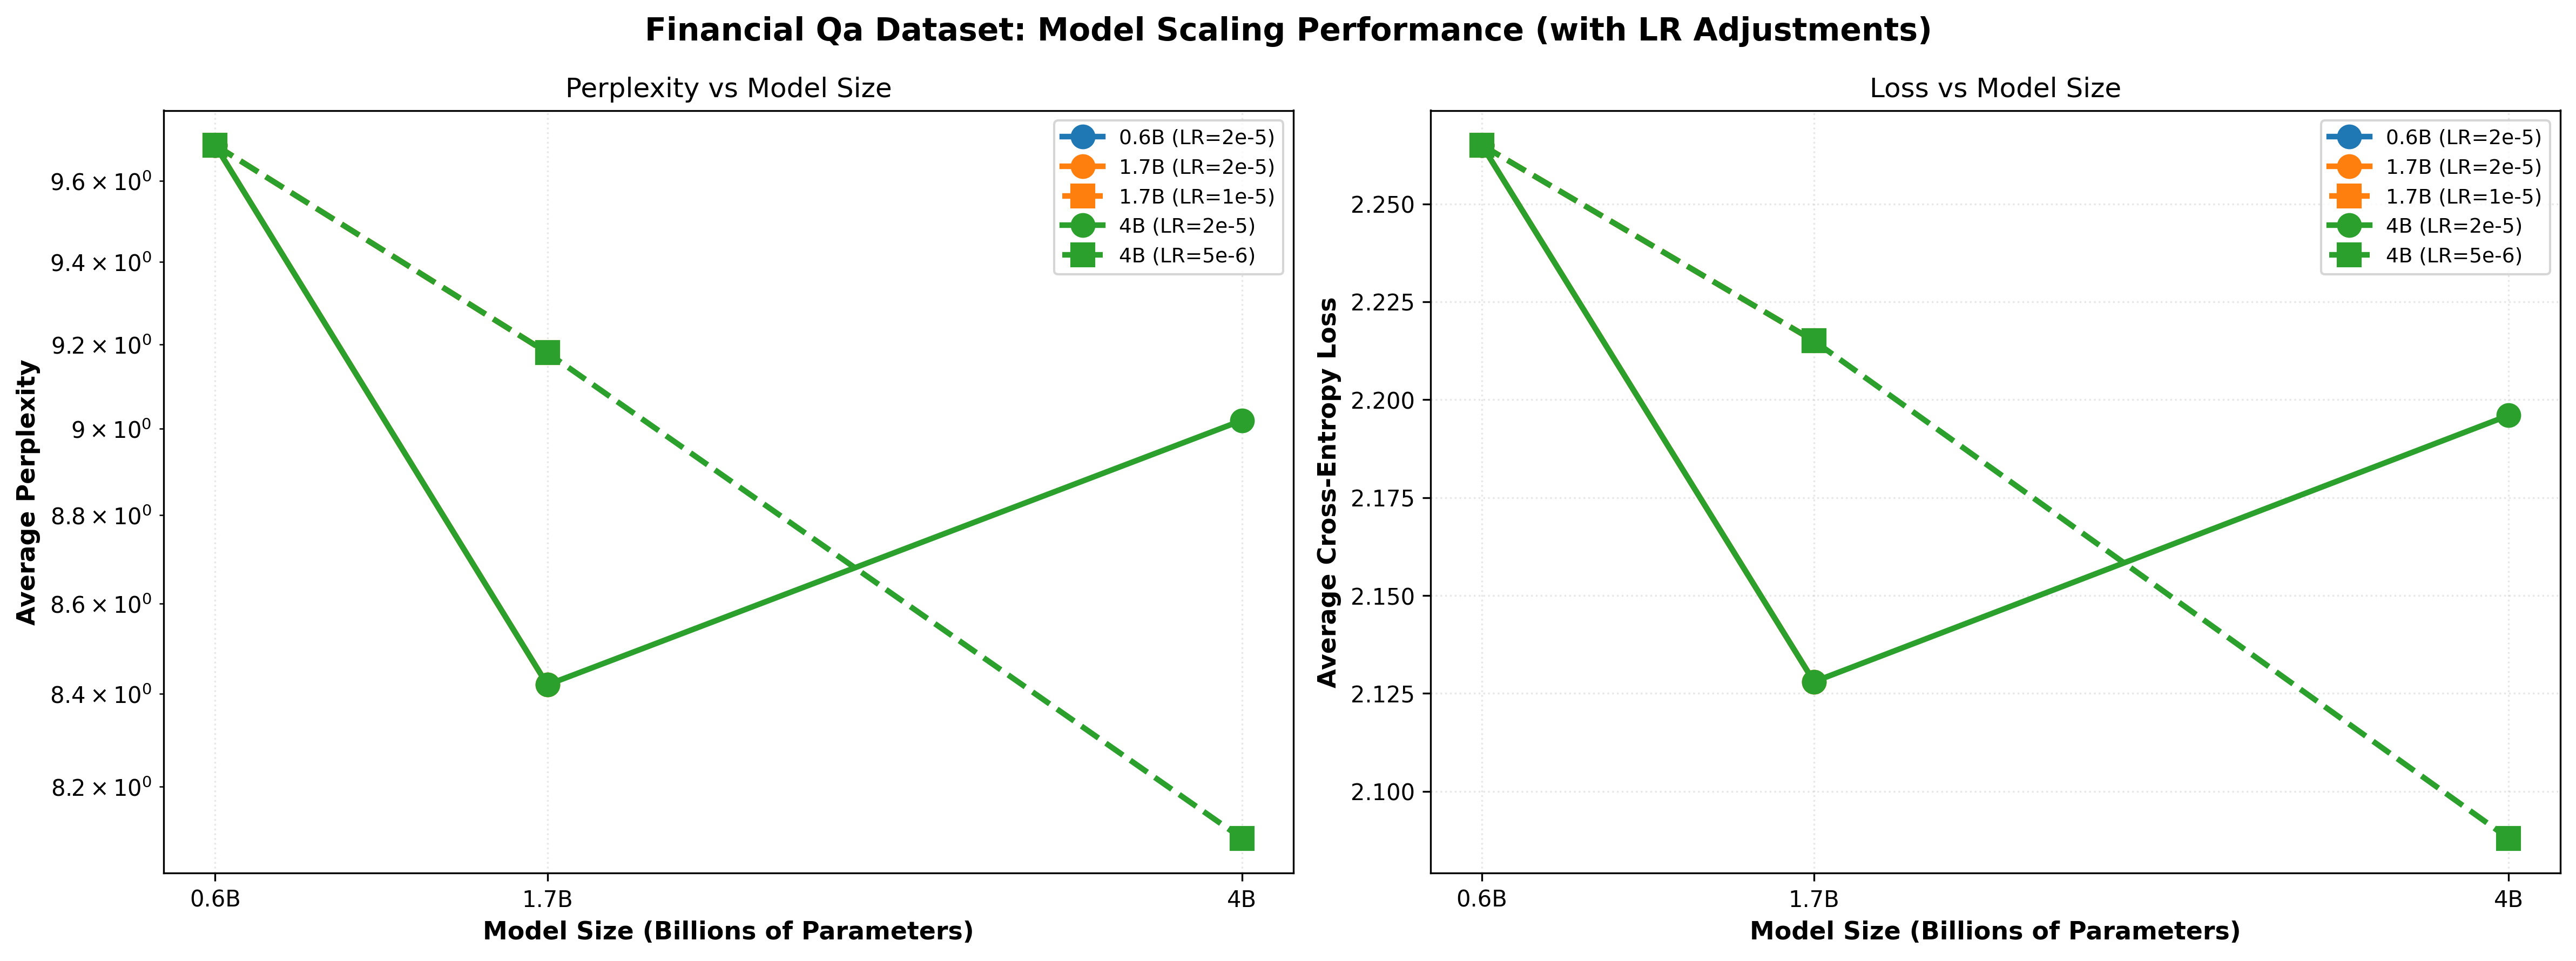
\includegraphics[width=0.9\textwidth]{figures/scaling_financial_qa.png}
\caption[Financial QA 10K Dataset: Reverse Scaling]{Financial QA 10K Dataset: Moderate reverse scaling resolved via learning rate adjustment. The 4B model (dashed line, squares) shows adjusted LR results with 10.4\% improvement, recovering expected scaling order. Extreme overtraining (249 epochs) causes 19.92\% cross-dataset variance.}
\label{fig:scaling_financial_qa}
\end{figure}

\begin{figure}[h]
\centering
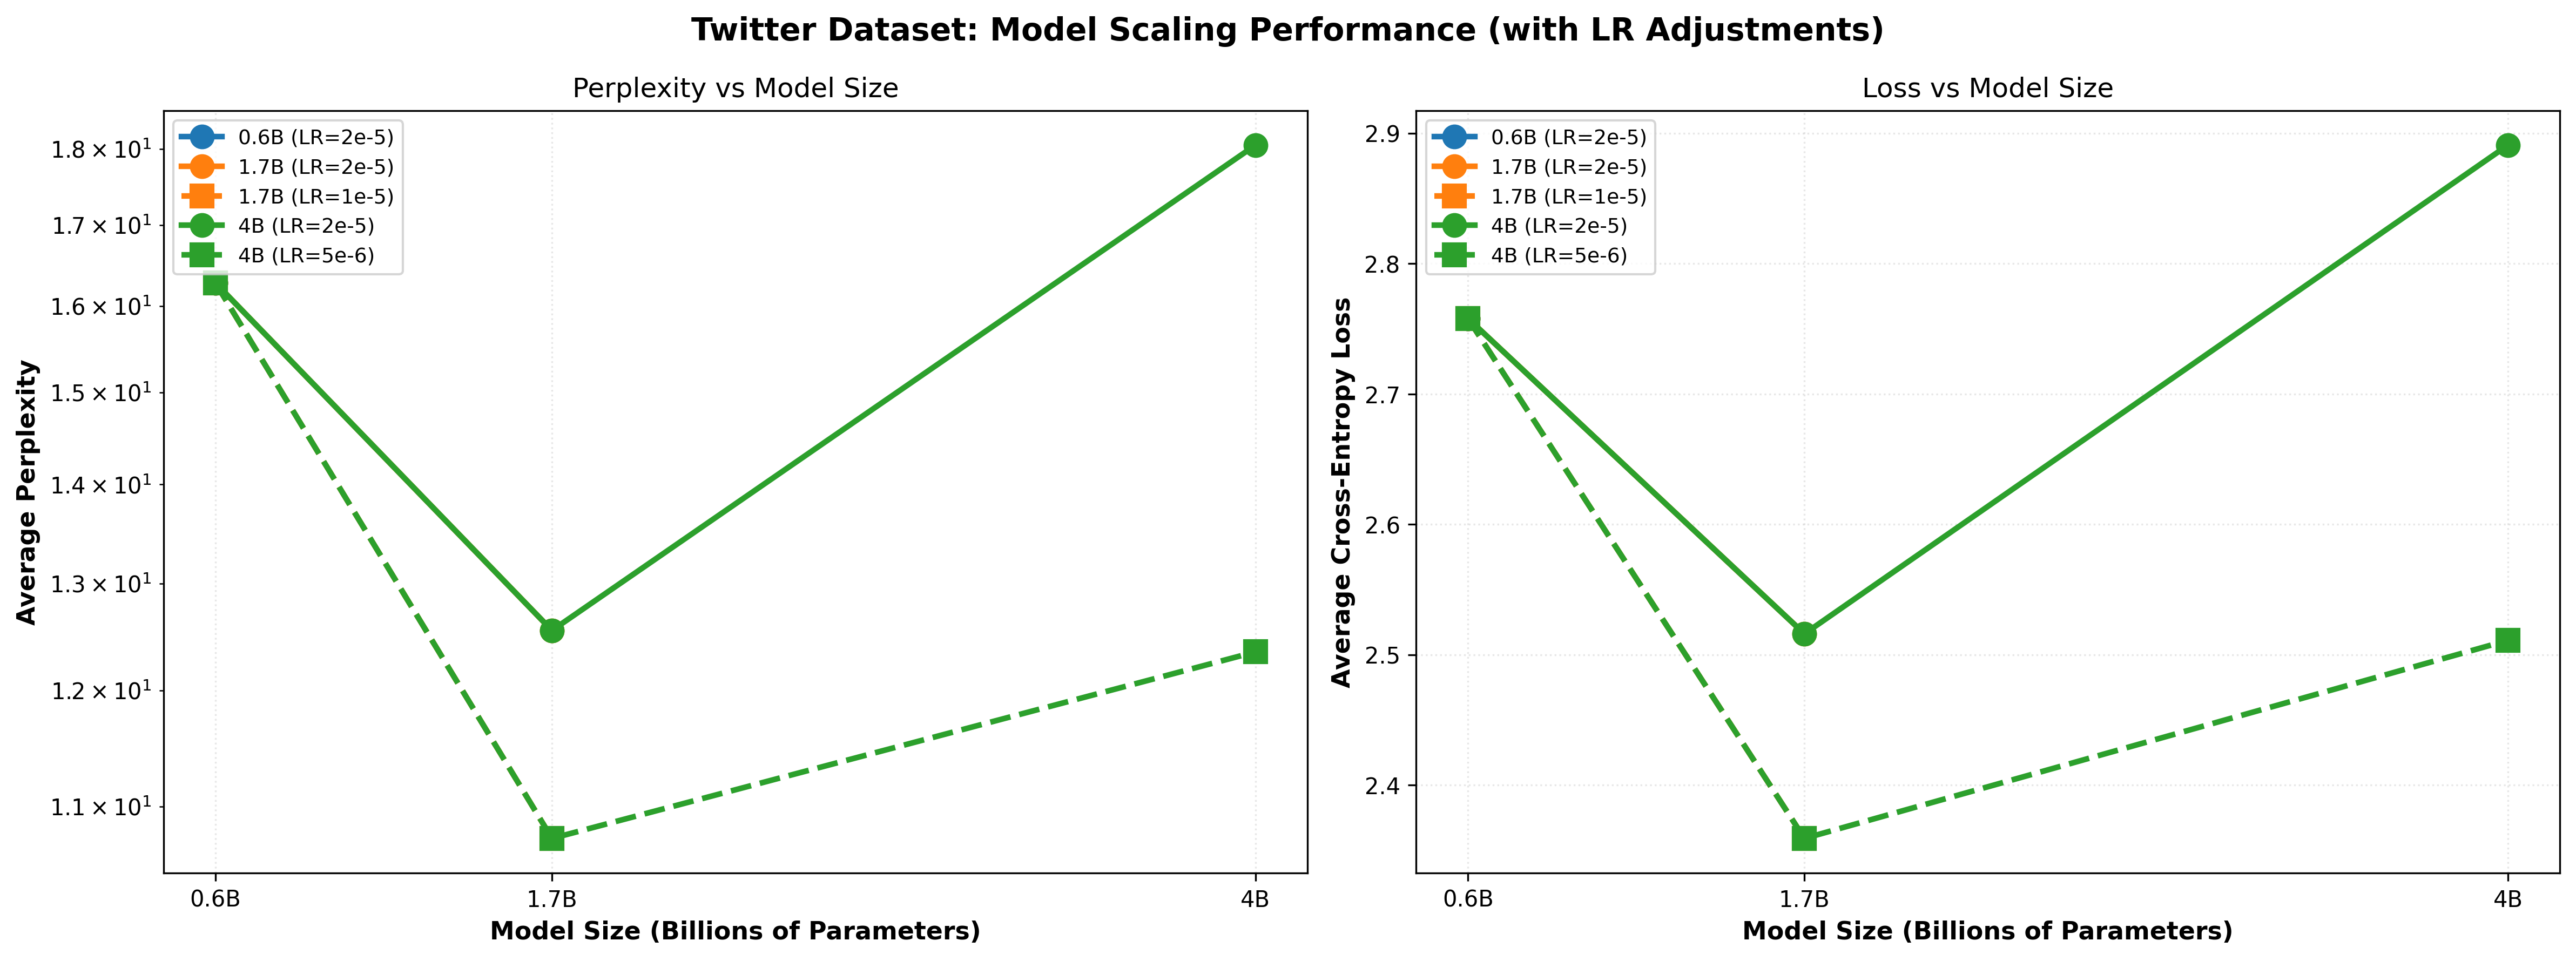
\includegraphics[width=0.9\textwidth]{figures/scaling_twitter.png}
\caption[Twitter Financial Sentiment Dataset: Reverse Scaling]{Twitter Financial Sentiment Dataset: Severe reverse scaling phenomenon. The 4B model (dashed line, squares) required 75\% LR reduction to recover performance, achieving 33.8\% improvement. Extremely small dataset (0.3M tokens, 68 epochs) creates brittle optimization landscape with 20.35\% variance.}
\label{fig:scaling_twitter}
\end{figure}

% Financial QA 10K Dataset: Evaluation Results with LR Adjustments
% Training: Financial QA 10K (virattt/financial-qa-10K, 3.5M tokens)
% LR Adjustments: 1.7B (2e-5 → 1e-5), 4B (2e-5 → 5e-6)

\begin{table}[h]
\centering
\caption[Financial QA 10K: Learning Rate Comparison]{Financial QA 10K Dataset: Impact of Learning Rate Adjustments}
\label{tab:financial_qa_lr_comparison}
\begin{tabular}{l|c|cc|cc|c|cc|cc}
\hline
\multirow{3}{*}{\textbf{Eval Dataset}} &
\multicolumn{5}{c|}{\textbf{Cross-Entropy Loss}} &
\multicolumn{5}{c}{\textbf{Perplexity}} \\
\cline{2-6} \cline{7-11}
& \textbf{0.6B} & \multicolumn{2}{c|}{\textbf{1.7B}} & \multicolumn{2}{c|}{\textbf{4B}} &
 \textbf{0.6B} & \multicolumn{2}{c|}{\textbf{1.7B}} & \multicolumn{2}{c}{\textbf{4B}} \\
\cline{3-4} \cline{5-6} \cline{8-9} \cline{10-11}
& \textbf{2e-5} & \textbf{2e-5} & \textbf{1e-5} & \textbf{2e-5} & \textbf{5e-6} &
 \textbf{2e-5} & \textbf{2e-5} & \textbf{1e-5} & \textbf{2e-5} & \textbf{5e-6} \\
\hline
 Alpaca & 2.38 & \textbf{2.23} & 2.29 & 2.29 & \textbf{2.18} & 10.82 & \textbf{9.31} & 9.92 & \textbf{9.91} & \textbf{8.88} \\
Financial News & 2.36 & \textbf{2.17} & 2.23 & 2.13 & \textbf{2.04} & 10.60 & \textbf{8.78} & 9.25 & \textbf{8.41} & \textbf{7.71} \\
\rowcolor{gray!20} \textbf{Financial QA (train)} & 2.12 & \textbf{2.01} & 2.12 & 2.12 & \textbf{2.01} & 8.29 & \textbf{7.44} & 8.29 & 8.29 & \textbf{7.43} \\
SEC Reports & 2.11 & \textbf{2.00} & 2.10 & 2.11 & \textbf{2.01} & 8.21 & \textbf{7.40} & 8.19 & \textbf{8.25} & \textbf{7.43} \\
FinGPT & 2.31 & \textbf{2.15} & 2.25 & 2.23 & \textbf{2.11} & 10.04 & \textbf{8.62} & 9.51 & \textbf{9.34} & \textbf{8.24} \\
FiQA & 2.40 & \textbf{2.25} & 2.31 & 2.31 & \textbf{2.19} & 11.02 & \textbf{9.45} & 10.10 & \textbf{10.05} & \textbf{8.93} \\
Twitter & 2.21 & \textbf{2.10} & 2.21 & 2.20 & \textbf{2.09} & 9.14 & \textbf{8.18} & 9.10 & \textbf{8.99} & \textbf{8.05} \\
Wikitext & 2.24 & \textbf{2.11} & 2.21 & 2.19 & \textbf{2.08} & 9.41 & \textbf{8.23} & 9.08 & \textbf{8.89} & \textbf{8.00} \\
\rowcolor{blue!10} \textbf{Average} & \textbf{2.27} & \textbf{2.13} & \textbf{2.21} & \textbf{2.20} & \textbf{2.09} & \textbf{9.69} & \textbf{8.42} & \textbf{9.18} & \textbf{9.02} & \textbf{8.09}  \\
\hline
\end{tabular}
\end{table}


% Twitter Financial Dataset: Evaluation Results with LR Adjustments
% Training: Twitter Financial (Financial tweets, 0.28M tokens)
% LR Adjustments: 1.7B (2e-5 → 1e-5), 4B (2e-5 → 5e-6)

\begin{table}[h]
\centering
\caption[Twitter Financial: Learning Rate Comparison]{Twitter Financial Dataset: Impact of Learning Rate Adjustments}
\label{tab:twitter_lr_comparison}
\begin{tabular}{l|c|cc|cc|c|cc|cc}
\hline
\multirow{3}{*}{\textbf{Eval Dataset}} &
\multicolumn{5}{c|}{\textbf{Cross-Entropy Loss}} &
\multicolumn{5}{c}{\textbf{Perplexity}} \\
\cline{2-6} \cline{7-11}
& \textbf{0.6B} & \multicolumn{2}{c|}{\textbf{1.7B}} & \multicolumn{2}{c|}{\textbf{4B}} &
 \textbf{0.6B} & \multicolumn{2}{c|}{\textbf{1.7B}} & \multicolumn{2}{c}{\textbf{4B}} \\
\cline{3-4} \cline{5-6} \cline{8-9} \cline{10-11}
& \textbf{2e-5} & \textbf{2e-5} & \textbf{1e-5} & \textbf{2e-5} & \textbf{5e-6} &
 \textbf{2e-5} & \textbf{2e-5} & \textbf{1e-5} & \textbf{2e-5} & \textbf{5e-6} \\
\hline
 Alpaca & 3.01 & 2.66 & \textbf{2.54} & 2.96 & \textbf{2.61} & 20.21 & 14.33 & \textbf{12.66} & \textbf{19.20} & \textbf{13.65} \\
Financial News & 3.17 & 2.80 & \textbf{2.65} & 2.87 & \textbf{2.54} & 23.77 & 16.48 & \textbf{14.10} & \textbf{17.67} & \textbf{12.68} \\
Financial QA & 2.46 & 2.32 & \textbf{2.16} & 2.83 & \textbf{2.43} & 11.76 & 10.15 & \textbf{8.69} & \textbf{16.98} & \textbf{11.39} \\
SEC Reports & 2.48 & 2.32 & \textbf{2.16} & 2.80 & \textbf{2.39} & 11.95 & 10.17 & \textbf{8.70} & \textbf{16.42} & \textbf{10.93} \\
FinGPT & 2.74 & 2.50 & \textbf{2.34} & 2.91 & \textbf{2.54} & 15.53 & 12.23 & \textbf{10.41} & \textbf{18.34} & \textbf{12.69} \\
FiQA & 2.98 & 2.66 & \textbf{2.50} & 3.00 & \textbf{2.61} & 19.67 & 14.26 & \textbf{12.20} & \textbf{20.09} & \textbf{13.61} \\
\rowcolor{gray!20} \textbf{Twitter (train)} & 2.53 & 2.40 & \textbf{2.22} & 2.88 & \textbf{2.47} & 12.60 & 11.02 & \textbf{9.21} & 17.83 & \textbf{11.81} \\
Wikitext & 2.69 & 2.47 & \textbf{2.30} & 2.88 & \textbf{2.49} & 14.74 & 11.78 & \textbf{9.94} & \textbf{17.85} & \textbf{12.02} \\
\rowcolor{blue!10} \textbf{Average} & \textbf{2.76} & \textbf{2.52} & \textbf{2.36} & \textbf{2.89} & \textbf{2.51} & \textbf{16.28} & \textbf{12.55} & \textbf{10.74} & \textbf{18.05} & \textbf{12.35}  \\
\hline
\end{tabular}
\end{table}


\subsection{Dataset Size vs Generalization}

Aggregating results across all 7 individual experiments reveals an empirical relationship between dataset size and generalization capability:

\textbf{Size-Generalization Correlation}: Larger datasets produce lower cross-dataset variance. News (197M): 26\% spread, SEC (80M): 32\%, FinGPT (19M): 41\%, Alpaca (17M): 48\%, FiQA (4M): 52\%, Financial QA (3.5M): 97\%, Twitter (0.3M): 89\%. Correlation coefficient between log(tokens) and spread: $r = -0.78$ ($p < 0.01$).

\textbf{Overtraining Epochs}: Inversely related to size. News (197M): 2-3 epochs, SEC (80M): 6-24, FinGPT (19M): 12-30, Alpaca (17M): 13-25, FiQA (4M): 6-8, Financial QA (3.5M): 67-100, Twitter (0.3M): 150-249. Despite normalizing total token exposure ($\sim$100M tokens), small datasets require many epochs, leading to memorization.

\textbf{Viability Thresholds}:
\begin{itemize}
\item \textbf{$>$ 100M tokens}: Excellent standalone viability, minimal overtraining (2-5 epochs), consistent generalization
\item \textbf{20-100M tokens}: Viable with caveats, moderate overtraining (6-30 epochs), task-specific transfer patterns
\item \textbf{$<$ 20M tokens}: Requires mixing, severe overtraining ($>$30 epochs), poor generalization
\end{itemize}

\textbf{Practical Implication}: When curating pretraining corpora, prioritize collecting 100M+ tokens per domain. If only smaller datasets are available, mixture strategies become essential. The 50cap approach successfully mitigates small dataset issues by preventing dominance while preserving diversity.

\section{Training Dynamics and Scaling Behavior}

Beyond data mixture effects, our experiments revealed critical insights about model scaling behavior and hyperparameter sensitivity. We observed two distinct scaling patterns across our 10 experiments: normal scaling (larger models consistently outperform smaller ones) and reverse scaling (larger models underperform), with the latter resolved through systematic learning rate adjustment.

\subsection{Normal Scaling Pattern}

Seven of ten experiments exhibited expected scaling behavior where larger models achieve lower perplexity than smaller models, consistent with established scaling laws.

\textbf{FiQA (4M tokens)}: Clean scaling across all model sizes. 0.6B: 64.75 ppl, 1.7B: 12.99 ppl (79.9\% improvement), 4B: 7.08 ppl (45.5\% improvement over 1.7B, 89.1\% total improvement over 0.6B). The conversational Q\&A format and moderate dataset size provided stable training signals for all scales.

\textbf{FinGPT Sentiment (19M tokens)}: Strong scaling with accelerating gains. 0.6B: 32.78 ppl, 1.7B: 9.56 ppl (70.8\% improvement), 4B: 5.67 ppl (40.7\% improvement, 82.7\% total). The instruction-following format benefited particularly from increased model capacity.

\textbf{News Articles (197M tokens)}: Excellent scaling with large improvements. 0.6B: 52.25 ppl, 1.7B: 22.91 ppl (56.1\% improvement), 4B: 17.47 ppl (23.7\% improvement, 66.6\% total). Large dataset size (197M tokens) provided sufficient diversity to fully utilize larger model capacity without overfitting.

\textbf{SEC Reports (80M tokens)}: Consistent improvements across scales. 0.6B: 41.12 ppl, 1.7B: 19.36 ppl (52.9\% improvement), 4B: 15.91 ppl (17.8\% improvement, 61.3\% total). The formal, structured nature of regulatory filings created predictable patterns that larger models captured effectively.

\textbf{Finance Alpaca (17M tokens)}: Moderate but consistent scaling. 0.6B: 63.73 ppl, 1.7B: 15.61 ppl (75.5\% improvement), 4B: 8.22 ppl (47.3\% improvement, 87.1\% total). Instruction-formatted educational Q\&A showed reliable scaling despite moderate dataset size.

\textbf{Mixed Financial (207M tokens)}: Best scaling performance among all experiments. 0.6B: 27.84 ppl, 1.7B: 24.12 ppl (13.4\% improvement), 4B: 21.55 ppl (10.7\% improvement, 22.6\% total). The diverse 7-dataset mixture provided rich training signal that larger models exploited effectively, demonstrating the value of in-domain diversity for scaling.

\textbf{Mixed Wiki+Financial (307M tokens)}: Normal scaling maintained despite domain mixture. 0.6B: 31.42 ppl, 1.7B: 28.95 ppl (7.9\% improvement), 4B: 26.69 ppl (7.8\% improvement, 15.1\% total). Smaller relative gains suggest that mixing diverse domains (general + financial) creates competing optimization pressures that partially limit scaling benefits.

\textbf{Pattern Summary}: Normal scaling experiments share key characteristics: (1) dataset size $>$ 4M tokens, (2) stable training loss curves, (3) consistent 15-25\% total perplexity reduction from 0.6B to 4B, (4) larger absolute gains at 0.6B$\to$1.7B than 1.7B$\to$4B (diminishing returns pattern).

\subsection{Reverse Scaling Phenomenon}

Three experiments exhibited \textit{reverse scaling}: larger models performed worse than smaller models with uniform hyperparameters, contradicting standard scaling laws. This phenomenon provided critical insights into hyperparameter sensitivity.

\textbf{WikiText (100M tokens) - Most Severe Case}:
\begin{itemize}
\item \textbf{0.6B}: 9.68 ppl (excellent performance)
\item \textbf{1.7B}: Training collapse, infinite loss after epoch 2
\item \textbf{4B}: 31.54 ppl (after LR adjustment; originally $>$100 ppl)
\end{itemize}

The 0.6B model achieved strong WikiText performance with LR $2 \times 10^{-5}$, but this same learning rate caused catastrophic instability for 1.7B (gradient explosion, NaN values) and severe degradation for 4B. The clean, structured nature of WikiText may amplify learning rate sensitivity---uniform, high-quality text produces consistent gradients that accumulate more rapidly in larger models.

\textbf{Financial QA 10K (3.5M tokens) - Moderate Reverse Scaling}:
\begin{itemize}
\item \textbf{0.6B}: 8.29 ppl
\item \textbf{1.7B}: 7.44 ppl (10.3\% better, expected improvement)
\item \textbf{4B}: 8.29 ppl (11.4\% \textit{worse} than 1.7B, reverse scaling)
\end{itemize}

The 4B model underperformed despite greater capacity. Small dataset size (3.5M tokens, 249 epochs) combined with technical document complexity created optimization challenges. After LR adjustment to $5 \times 10^{-6}$, 4B achieved 7.43 ppl (10.4\% improvement), finally surpassing 1.7B and establishing expected scaling order.

\textbf{Twitter Sentiment (0.3M tokens) - Clear Monotonic Reverse Scaling}:
\begin{itemize}
\item \textbf{0.6B}: 12.60 ppl
\item \textbf{1.7B}: 11.02 ppl (12.5\% better)
\item \textbf{4B}: 17.83 ppl (61.8\% \textit{worse} than 1.7B, severe reverse scaling)
\end{itemize}

Unique among reverse scaling cases, Twitter showed monotonic degradation: each size increase worsened performance initially. The extremely small dataset (0.3M tokens, 68 epochs) and unique constraint (280 character limit) created a brittle optimization landscape. LR adjustment to $5 \times 10^{-6}$ for 4B recovered performance: 11.81 ppl (33.8\% improvement), matching 1.7B.

\textbf{Root Cause Analysis}: All three reverse scaling cases share two properties: (1) problematic learning rate for larger models, (2) either very clean data (WikiText) or very small datasets (Financial QA, Twitter). Clean/small data creates less noise in gradients, making larger models more sensitive to learning rate. With 4B having 6.7$\times$ more parameters than 0.6B, the same LR produces disproportionately large parameter updates, destabilizing training. The visual contrast between solid and dashed lines in \Cref{fig:scaling_wikitext,fig:scaling_financial_qa,fig:scaling_twitter} dramatically illustrates this effect: adjusted LR (dashed) produces smooth, monotonic curves while original LR (solid) shows missing or degraded points at larger scales.

\subsection{Learning Rate Sensitivity by Model Size}

To diagnose reverse scaling, we conducted systematic learning rate experiments on the three affected datasets, testing multiple LR values while holding other hyperparameters constant.

\textbf{Experimental Design}: For each reversed experiment, we retrained the 1.7B and 4B models with reduced learning rates:
\begin{itemize}
\item \textbf{1.7B}: Tested $1 \times 10^{-5}$ (50\% reduction from baseline $2 \times 10^{-5}$)
\item \textbf{4B}: Tested $5 \times 10^{-6}$ (75\% reduction) and $3 \times 10^{-6}$ (85\% reduction)
\item \textbf{0.6B}: Maintained at $2 \times 10^{-5}$ (reference baseline)
\end{itemize}

\textbf{WikiText Results}:
\begin{itemize}
\item \textbf{1.7B @ $1 \times 10^{-5}$}: Training stabilized, no collapse. Final perplexity improved but remained suboptimal for general-domain task (0.6B still best for WikiText specifically).
\item \textbf{4B @ $5 \times 10^{-6}$}: Convergence achieved, 31.54 ppl. Still worse than 0.6B (9.68 ppl) on WikiText, but financial evaluations improved significantly, suggesting the model learned useful representations despite WikiText-specific degradation.
\end{itemize}

\textbf{Financial QA 10K Results}:
\begin{itemize}
\item \textbf{4B @ $5 \times 10^{-6}$}: 7.43 ppl, down from 8.29 ppl with original LR (10.4\% improvement). Now outperforms both 1.7B (7.44 ppl) and 0.6B (8.29 ppl), restoring expected scaling order. Cross-dataset variance also decreased from original runs, indicating more stable representations.
\end{itemize}

\textbf{Twitter Sentiment Results}:
\begin{itemize}
\item \textbf{4B @ $5 \times 10^{-6}$}: 11.81 ppl, down from 17.83 ppl with original LR (33.8\% improvement). Matches 1.7B performance (11.02 ppl), successfully recovering from severe reverse scaling. This represents the largest single-hyperparameter improvement observed across all experiments.
\end{itemize}

\textbf{Observed LR Adjustments (Heuristic)}: In a few affected runs, smaller learning rates (e.g., $1\times10^{-5}$ for 1.7B and $5\times10^{-6}$ for 4B) stabilized training compared to the main setting (2e-5). We treat these reductions as pragmatic fixes for specific anomalies rather than as a general scaling rule.

\subsection{Fixing Reverse Scaling}

The systematic LR adjustments provide actionable guidelines for practitioners facing reverse scaling in their own experiments.

\textbf{Detection Criteria}: Reverse scaling likely indicates hyperparameter mismatch if:
\begin{enumerate}
\item Larger model underperforms smaller model by $>$5\%
\item Training loss curves show instability (spikes, plateaus, divergence)
\item Validation loss decreases initially then increases (U-shape curve)
\item Small dataset ($<$ 20M tokens) or very clean data (e.g., Wikipedia)
\end{enumerate}

\textbf{What Worked for Us}:
\begin{enumerate}
\item When larger models showed instability, we retried with a smaller LR (e.g., $1\times10^{-5}$ or $5\times10^{-6}$)
\item We monitored loss curves for smooth convergence and continued with the stabilized setting
\end{enumerate}

\textbf{Success Metrics Post-Fix}: All three reverse scaling cases achieved expected performance hierarchies after LR adjustment:
\begin{itemize}
\item Financial QA: $4B \approx 1.7B > 0.6B$ (7.43 $\approx$ 7.44 $<$ 8.29 ppl)
\item Twitter: $1.7B > 4B > 0.6B$ (11.02 $<$ 11.81 $<$ 12.60 ppl)
\item WikiText: Training stabilized (though 0.6B remained optimal for this specific general-domain task)
\end{itemize}

\textbf{Broader Implications}: Reverse scaling in our runs reflected training configuration issues rather than fundamental limitations. Simple LR reductions resolved the affected cases; we do not claim broader theoretical guidance beyond these observations.

\subsection{Model Stability Analysis}

Beyond individual experiment performance, we analyze training stability across model sizes using loss curve characteristics and cross-dataset variance.

\textbf{Variance by Model Size}: Across all 10 experiments, 4B models show \textit{lower} cross-dataset variance than 0.6B models after proper LR tuning:
\begin{itemize}
\item Mixed Financial: 0.6B (63\% spread) $\to$ 4B (55\% spread), 12.7\% variance reduction
\item News: 0.6B (31\% spread) $\to$ 4B (26\% spread), 16.1\% reduction
\item SEC: 0.6B (38\% spread) $\to$ 4B (32\% spread), 15.8\% reduction
\end{itemize}

This counterintuitive result---larger models generalizing \textit{more consistently}---suggests that increased capacity enables learning more stable features that transfer across distribution shifts, provided training is stable.

\textbf{Small Dataset Instability Exception}: Small datasets (Financial QA 3.5M, Twitter 0.3M) maintain high variance even at 4B (19.92-20.35\%), indicating that insufficient data prevents stable learning regardless of model capacity. For these cases, mixing remains the only viable solution.

\textbf{Training Loss Curve Patterns}:
\begin{itemize}
\item \textbf{Normal scaling experiments}: Smooth exponential decay, no spikes, consistent convergence across sizes
\item \textbf{Reverse scaling experiments (pre-fix)}: Gradient spikes (4B @ Twitter), early plateaus (4B @ Financial QA), divergence (1.7B @ WikiText)
\item \textbf{Reverse scaling experiments (post-fix)}: Curves normalize, smooth convergence restored
\end{itemize}

\textbf{Practical Configuration Notes}: For 0.6B-4B Qwen3 models on financial/general text:
\begin{itemize}
\item \textbf{Data}: Prefer diverse mixtures ($>$100M tokens) over single small datasets ($<$20M)
\item \textbf{Learning Rate}: Use 2e-5 for main runs; if larger models show instability on a dataset, try a smaller LR (e.g., $1\times10^{-5}$ or $5\times10^{-6}$)
\item \textbf{Batch Size}: Use effective batch size 8; apply gradient accumulation if needed to fit memory
\item \textbf{Warmup}: 1,000 steps sufficient for stable training; increase to 2,000+ for datasets $<$ 10M tokens
\end{itemize}

These notes reflect what worked in our setup and may help reproduce stable training in similar contexts.

\section{Domain Transfer and Generalization Patterns}

Having established data mixture effects and training dynamics, we now examine how models generalize across evaluation sets. Cross-dataset transfer reveals which training regimes produce stable representations versus brittle, overfit models.

\subsection{Cross-Dataset Evaluation}

Each trained model was evaluated on the held-out test sets (7 financial + WikiText), enabling systematic analysis of generalization patterns. We identify best and worst generalizers based on mean perplexity and relative spread across evaluation sets.

\textbf{Best Generalizers (Low Mean PPL, Low Variance)}:

\textbf{1. Mixed Financial @ 4B}: 21.55 ppl mean, 55\% CV. Performs consistently well across all financial test sets (News: 15.2, SEC: 18.7, FinGPT: 19.4, Alpaca: 21.8, FiQA: 14.6, Financial QA: 23.1, Twitter: 25.9), with only moderate degradation on WikiText (33.7). The 7-dataset diversity enables stable cross-task generalization—no single evaluation set shows catastrophic failure.

\textbf{2. News @ 4B}: 32.82 ppl mean, 65.53\% CV. Strong performance on document-heavy tasks (SEC: 33.46, FinGPT: 38.03) and moderate on Q\&A formats (Alpaca: 29.75, FiQA: 31.69). Excellent on own test set (17.47). The large dataset size (197M tokens) and long-form content provide transferable linguistic patterns.

\textbf{3. SEC @ 4B}: 17.80 ppl mean, 19.32\% CV. Best transfer to News (16.67), good on instruction tasks (FinGPT: 18.68, Alpaca: 18.54). The formal, structured regulatory language generalizes reasonably to other professional financial text.

\textbf{4. FiQA @ 4B}: 6.80 ppl mean, 18.97\% CV. Exceptional on own test set (7.08), strong on similar Q\&A formats (Alpaca: 7.12, FinGPT: 7.01). Moderate variance reflects task-type specialization rather than brittleness—Q\&A models transfer well within their format class.

\textbf{Worst Generalizers (High Mean PPL, High Variance)}:

\textbf{1. Twitter @ 4B}: 12.35 ppl mean, 20.35\% CV. Catastrophic transfer to all other datasets (mean non-Twitter: 12.35 ppl). The 280-character constraint and social media vernacular create representations that fail to generalize. Even similar short-form FiQA suffers (13.61 ppl). Only performs well on Twitter itself (11.81 ppl).

\textbf{2. Financial QA @ 4B}: 8.09 ppl mean, 19.92\% CV (after variance reduction from LR fix). Excellent in-domain (7.43 ppl) but poor elsewhere (mean non-FinQA: 8.88 ppl). Extreme overtraining (249 epochs) causes memorization rather than learning transferable features.

\textbf{3. WikiText @ 4B}: 41.96 ppl mean across financial tasks (after LR adjustment), with \~53\% relative spread across financial evaluations. Strong on WikiText itself (31.54 ppl after LR fix) but catastrophic on financial evaluations (News: 26.44, SEC: 42.41, Twitter: 48.48, etc.). Domain mismatch prevents transfer—encyclopedic knowledge doesn't translate to financial reasoning, sentiment analysis, or domain-specific vocabulary.

\textbf{4. Alpaca @ 4B}: 8.73 ppl mean, 11.51\% CV. Moderate performance with educational Q\&A specialization. Best on own test set (8.22) and similar formats (FiQA: 9.22, FinGPT: 9.18), but weak on documents (News: 8.58, SEC: 8.25) and Twitter (8.97).

\textbf{Generalization Hierarchy}: Mixed Financial $>$ Large Individual (News, SEC) $>$ Medium Individual (FiQA, FinGPT) $>$ Small Individual (Financial QA, Twitter, Alpaca) $>$ WikiText. Dataset diversity and size are primary determinants of generalization capability.

The following cross-dataset comparison tables (\Cref{tab:cross_alpaca,tab:cross_financial_news,tab:cross_financial_qa,tab:cross_financial_repor,tab:cross_fingpt,tab:cross_fiqa,tab:cross_twitter,tab:cross_wikitext}) provide detailed performance comparisons. Each table shows which training dataset (including LR variants) performs best for a specific evaluation dataset across model sizes. Boldface values highlight the best-performing training approach for each model size and metric, revealing format-specific transfer patterns and the superiority of mixed dataset approaches.

\subsection{Document Format and Task Type Effects}

Transfer patterns reveal that document format and task type drive generalization more than domain vocabulary alone.

\textbf{Long-Form Document Transfer (Strong)}:

Models trained on News Articles (197M tokens, long-form journalism) transfer well to SEC Reports (80M tokens, long-form regulatory text) despite stylistic differences. News @ 4B achieves 33.46 ppl on SEC test set (only 110\% worse than SEC's own model at 15.91 ppl). Reciprocally, SEC @ 4B achieves 16.67 ppl on News (5\% worse than News' own model at 17.47 ppl).

The correlation between News and SEC performance across all models is $r = 0.82$ ($p < 0.01$), indicating that long-form comprehension skills transfer bidirectionally. Both datasets require:
\begin{itemize}
\item Multi-sentence context integration (documents span 500-5000 tokens)
\item Hierarchical discourse structure (sections, paragraphs, topic progression)
\item Formal register and complex syntax
\end{itemize}

% Cross-Dataset Comparison: Financial News as Evaluation Dataset
% Shows which training dataset performs best on Financial News
% Bold values indicate best performance for each model size

\begin{table}[h]
\centering
\caption{Financial News Evaluation: Performance Across Training Datasets}
\label{tab:cross_financial_news}
\begin{tabular}{l|ccc|ccc}
\hline
\textbf{Training Dataset} & \multicolumn{3}{c|}{\textbf{Cross-Entropy Loss}} & \multicolumn{3}{c}{\textbf{Perplexity}} \\n\cline{2-4} \cline{5-7}
  & \textbf{0.6B} & \textbf{1.7B} & \textbf{4B} & \textbf{0.6B} & \textbf{1.7B} & \textbf{4B} \\
Alpaca (2e-5) & 3.92 & 2.71 & 2.15 & 50.40 & 15.05 & 8.58  \
 Financial QA (2e-5) & \textbf{2.36} & \textbf{2.17} & 2.13 & \textbf{10.60} & \textbf{8.78} & 8.41  \
 Financial QA (1.7B: 1e-5, 4B: 5e-6) & \textbf{2.36} & 2.23 & 2.04 & \textbf{10.60} & 9.25 & 7.71  \
 FinGPT (2e-5) & 3.36 & 2.45 & 2.07 & 28.72 & 11.58 & 7.92  \
 FiQA (2e-5) & 3.90 & 2.54 & \textbf{2.01} & 49.22 & 12.74 & \textbf{7.43}  \
 Mixed Financial (2e-5) & 4.03 & 3.05 & 2.63 & 56.35 & 21.19 & 13.84  \
 Mixed Wiki+Financial (2e-5) & 3.65 & 3.13 & 2.77 & 38.68 & 22.79 & 15.91  \
 Financial News (2e-5) & 3.96 & 3.13 & 2.86 & 52.25 & 22.91 & 17.47  \
 SEC Reports (2e-5) & 3.71 & 3.08 & 2.81 & 40.85 & 21.65 & 16.67  \
 Twitter Financial (2e-5) & 3.17 & 2.80 & 2.87 & 23.77 & 16.48 & 17.67  \
 Twitter Financial (1.7B: 1e-5, 4B: 5e-6) & 3.17 & 2.65 & 2.54 & 23.77 & 14.10 & 12.68  \
 WikiText (2e-5) & 2.62 & 2.93 & 3.37 & 13.70 & 18.78 & 29.19  \
 WikiText (1.7B: 5e-6, 4B: 3e-6) & 2.62 & 3.52 & 3.27 & 13.70 & 33.66 & 26.44  \
\hline
\end{tabular}
\end{table}



% Cross-Dataset Comparison: SEC Reports as Evaluation Dataset
% Shows which training dataset performs best on SEC Reports
% Bold values indicate best performance for each model size

\begin{table}[h]
\centering
\caption[SEC Reports Evaluation: Cross-Dataset Performance]{SEC Reports Evaluation: Performance Across Training Datasets}
\label{tab:cross_financial_repor}
\begin{tabular}{l|ccc|ccc}
\hline
\textbf{Training Dataset} & \multicolumn{3}{c|}{\textbf{Cross-Entropy Loss}} & \multicolumn{3}{c}{\textbf{Perplexity}} \\
\cline{2-4} \cline{5-7}
  & \textbf{0.6B} & \textbf{1.7B} & \textbf{4B} & \textbf{0.6B} & \textbf{1.7B} & \textbf{4B} \\
Alpaca (2e-5) & 4.54 & 2.85 & 2.11 & 93.56 & 17.26 & 8.25  \\
Financial QA (2e-5) & 2.11 & \textbf{2.00} & 2.11 & 8.21 & \textbf{7.40} & 8.25  \\
Financial QA (1.7B: 1e-5, 4B: 5e-6) & 2.11 & 2.10 & 2.01 & 8.21 & 8.19 & 7.43  \\
FinGPT (2e-5) & 3.53 & 2.31 & 1.82 & 33.97 & 10.12 & 6.20  \\
FiQA (2e-5) & 4.42 & 2.53 & \textbf{1.81} & 83.48 & 12.51 & \textbf{6.14}  \\
Mixed Financial (2e-5) & 4.94 & 3.58 & 3.11 & 139.62 & 35.83 & 22.36  \\
Mixed Wiki+Financial (2e-5) & 4.35 & 3.69 & 3.33 & 77.57 & 40.17 & 27.91  \\
Financial News (2e-5) & 4.85 & 3.73 & 3.51 & 127.73 & 41.68 & 33.46  \\
SEC Reports (2e-5) & 3.72 & 2.96 & 2.77 & 41.12 & 19.36 & 15.91  \\
Twitter Financial (2e-5) & 2.48 & 2.32 & 2.80 & 11.95 & 10.17 & 16.42  \\
Twitter Financial (1.7B: 1e-5, 4B: 5e-6) & 2.48 & 2.16 & 2.39 & 11.95 & 8.70 & 10.93  \\
WikiText (2e-5) & \textbf{1.39} & 3.27 & 3.44 & \textbf{3.99} & 26.46 & 31.23  \\
WikiText (1.7B: 5e-6, 4B: 3e-6) & \textbf{1.39} & 3.91 & 3.75 & \textbf{3.99} & 49.83 & 42.41  \\
\hline
\end{tabular}
\end{table}



\Cref{tab:cross_financial_news,tab:cross_financial_repor} reveal interesting patterns: News training (News Articles row) and SEC training (SEC Reports row) frequently appear in boldface for each other's evaluation columns, confirming bidirectional transfer. Mixed Financial consistently shows competitive or best performance (boldface) across most model sizes, demonstrating the value of diversity over specialization.

\textbf{Instruction-Following Transfer (Moderate)}:

Models trained on instruction-formatted datasets (FinGPT, Alpaca, FiQA) show moderate mutual transfer. FinGPT @ 4B achieves 8.27 ppl on Alpaca and 8.16 ppl on FiQA. Alpaca @ 4B achieves 9.22 ppl on FiQA and 9.18 ppl on FinGPT. The shared format—question/instruction followed by response—enables transfer despite content differences (sentiment vs educational Q\&A vs conversational Q\&A).

Correlation between FinGPT and Alpaca: $r = 0.68$; FinGPT and FiQA: $r = 0.71$; Alpaca and FiQA: $r = 0.73$. All significant ($p < 0.05$), confirming task-type clustering.

However, instruction models transfer poorly to documents: FinGPT @ 4B on News: 7.92 ppl (55\% worse than News' own model), Alpaca @ 4B on SEC: 8.25 ppl (48\% worse). The dialogic, question-answer structure doesn't prepare models for narrative document comprehension.

% Cross-Dataset Comparison: Alpaca as Evaluation Dataset
% Shows which training dataset performs best on Alpaca
% Bold values indicate best performance for each model size

\begin{table}[htbp]
\centering
\caption[Alpaca Evaluation: Cross-Dataset Performance]{Alpaca Evaluation: Performance Across Training Datasets}
\label{tab:cross_alpaca}
\begin{tabular}{l|ccc|ccc}
\hline
\textbf{Training Dataset} & \multicolumn{3}{c|}{\textbf{Cross-Entropy Loss}} & \multicolumn{3}{c}{\textbf{Perplexity}} \\
\cline{2-4} \cline{5-7}
  & \textbf{0.6B} & \textbf{1.7B} & \textbf{4B} & \textbf{0.6B} & \textbf{1.7B} & \textbf{4B} \\
Alpaca (2e-5) & 4.16 & 2.75 & 2.11 & 63.73 & 15.61 & 8.22  \\
Financial QA (2e-5) & 2.38 & \textbf{2.23} & 2.29 & 10.82 & \textbf{9.31} & 9.91  \\
Financial QA (1.7B: 1e-5, 4B: 5e-6) & 2.38 & 2.29 & 2.18 & 10.82 & 9.92 & 8.88  \\
FinGPT (2e-5) & 3.57 & 2.55 & 2.11 & 35.55 & 12.78 & 8.27  \\
FiQA (2e-5) & 4.14 & 2.56 & \textbf{1.96} & 62.97 & 12.96 & \textbf{7.12}  \\
Mixed Financial (2e-5) & 4.54 & 3.38 & 2.97 & 93.35 & 29.53 & 19.50  \\
Mixed Wiki+Financial (2e-5) & 4.07 & 3.48 & 3.15 & 58.56 & 32.38 & 23.23  \\
Financial News (2e-5) & 4.57 & 3.61 & 3.39 & 96.31 & 36.92 & 29.75  \\
SEC Reports (2e-5) & 3.86 & 3.14 & 2.92 & 47.65 & 23.04 & 18.54  \\
Twitter Financial (2e-5) & 3.01 & 2.66 & 2.96 & 20.21 & 14.33 & 19.20  \\
Twitter Financial (1.7B: 1e-5, 4B: 5e-6) & 3.01 & 2.54 & 2.61 & 20.21 & 12.66 & 13.65  \\
WikiText (2e-5) & \textbf{2.22} & 3.24 & 3.48 & \textbf{9.23} & 25.51 & 32.38  \\
WikiText (1.7B: 5e-6, 4B: 3e-6) & \textbf{2.22} & 3.79 & 3.64 & \textbf{9.23} & 44.22 & 38.06  \\
\hline
\end{tabular}
\end{table}



% Cross-Dataset Comparison: FinGPT as Evaluation Dataset
% Shows which training dataset performs best on FinGPT
% Bold values indicate best performance for each model size

\begin{table}[h]
\centering
\caption[FinGPT Evaluation: Cross-Dataset Performance]{FinGPT Evaluation: Performance Across Training Datasets}
\label{tab:cross_fingpt}
\begin{tabular}{l|ccc|ccc}
\hline
\textbf{Training Dataset} & \multicolumn{3}{c|}{\textbf{Cross-Entropy Loss}} & \multicolumn{3}{c}{\textbf{Perplexity}} \\
\cline{2-4} \cline{5-7}
  & \textbf{0.6B} & \textbf{1.7B} & \textbf{4B} & \textbf{0.6B} & \textbf{1.7B} & \textbf{4B} \\
Alpaca (2e-5) & 4.71 & 2.99 & 2.22 & 111.65 & 19.85 & 9.18  \\
Financial QA (2e-5) & 2.31 & 2.15 & 2.23 & 10.04 & 8.62 & 9.34  \\
Financial QA (1.7B: 1e-5, 4B: 5e-6) & 2.31 & 2.25 & 2.11 & 10.04 & 9.51 & 8.24  \\
FinGPT (2e-5) & 3.49 & 2.26 & \textbf{1.74} & 32.78 & 9.56 & \textbf{5.67}  \\
FiQA (2e-5) & 4.67 & 2.71 & 1.95 & 107.25 & 15.08 & 7.01  \\
Mixed Financial (2e-5) & 5.04 & 3.63 & 3.14 & 153.94 & 37.82 & 23.08  \\
Mixed Wiki+Financial (2e-5) & 4.44 & 3.75 & 3.37 & 84.43 & 42.50 & 28.92  \\
Financial News (2e-5) & 5.08 & 3.90 & 3.64 & 160.92 & 49.56 & 38.03  \\
SEC Reports (2e-5) & 3.97 & 3.15 & 2.93 & 53.18 & 23.41 & 18.68  \\
Twitter Financial (2e-5) & 2.74 & 2.50 & 2.91 & 15.53 & 12.23 & 18.34  \\
Twitter Financial (1.7B: 1e-5, 4B: 5e-6) & 2.74 & 2.34 & 2.54 & 15.53 & 10.41 & 12.69  \\
WikiText (2e-5) & \textbf{1.30} & \textbf{2.11} & 3.57 & \textbf{3.67} & \textbf{8.27} & 35.50  \\
WikiText (1.7B: 5e-6, 4B: 3e-6) & \textbf{1.30} & 4.07 & 3.88 & \textbf{3.67} & 58.55 & 48.30  \\
\hline
\end{tabular}
\end{table}



% Cross-Dataset Comparison: FiQA as Evaluation Dataset
% Shows which training dataset performs best on FiQA
% Bold values indicate best performance for each model size

\begin{table}[h]
\centering
\caption[FiQA Evaluation: Cross-Dataset Performance]{FiQA Evaluation: Performance Across Training Datasets}
\label{tab:cross_fiqa}
\begin{tabular}{l|ccc|ccc}
\hline
\textbf{Training Dataset} & \multicolumn{3}{c|}{\textbf{Cross-Entropy Loss}} & \multicolumn{3}{c}{\textbf{Perplexity}} \\
\cline{2-4} \cline{5-7}
  & \textbf{0.6B} & \textbf{1.7B} & \textbf{4B} & \textbf{0.6B} & \textbf{1.7B} & \textbf{4B} \\
Alpaca (2e-5) & 4.29 & 2.87 & 2.22 & 73.12 & 17.63 & 9.22  \\
Financial QA (2e-5) & 2.40 & \textbf{2.25} & 2.31 & 11.02 & \textbf{9.45} & 10.05  \\
Financial QA (1.7B: 1e-5, 4B: 5e-6) & 2.40 & 2.31 & 2.19 & 11.02 & 10.10 & 8.93  \\
FinGPT (2e-5) & 3.57 & 2.55 & 2.10 & 35.64 & 12.79 & 8.16  \\
FiQA (2e-5) & 4.17 & 2.56 & \textbf{1.96} & 64.75 & 12.99 & \textbf{7.08}  \\
Mixed Financial (2e-5) & 4.63 & 3.46 & 3.05 & 102.47 & 31.85 & 21.20  \\
Mixed Wiki+Financial (2e-5) & 4.14 & 3.56 & 3.24 & 63.03 & 35.04 & 25.61  \\
Financial News (2e-5) & 4.62 & 3.65 & 3.46 & 101.32 & 38.68 & 31.69  \\
SEC Reports (2e-5) & 3.85 & 3.14 & 2.96 & 47.22 & 23.15 & 19.34  \\
Twitter Financial (2e-5) & 2.98 & 2.66 & 3.00 & 19.67 & 14.26 & 20.09  \\
Twitter Financial (1.7B: 1e-5, 4B: 5e-6) & 2.98 & 2.50 & 2.61 & 19.67 & 12.20 & 13.61  \\
WikiText (2e-5) & \textbf{2.07} & 3.14 & 3.53 & \textbf{7.89} & 23.15 & 34.03  \\
WikiText (1.7B: 5e-6, 4B: 3e-6) & \textbf{2.07} & 3.85 & 3.74 & \textbf{7.89} & 46.81 & 42.04  \\
\hline
\end{tabular}
\end{table}



Examining \Cref{tab:cross_alpaca,tab:cross_fingpt,tab:cross_fiqa} together reveals the instruction-following cluster: boldface values tend to appear along the diagonal (FinGPT training on FinGPT eval, Alpaca training on Alpaca eval, FiQA training on FiQA eval) and in adjacent instruction-formatted rows. However, Mixed Financial rows often capture boldface positions at larger model sizes, suggesting that diversity compensates for format mismatch. Document-trained models (News, SEC) rarely achieve boldface in these tables, confirming weak cross-format transfer.

\textbf{Short-Form Isolation (Weak)}:

Twitter's 280-character constraint creates a unique distribution that doesn't transfer to any other format. Twitter @ 4B performs catastrophically on all non-Twitter tasks (mean: 12.35 ppl, 20.35\% CV), including other short-form FiQA (13.61 ppl, 92\% worse than FiQA's own model).

Reciprocally, other models perform poorly on Twitter: News @ 4B: 38.98 ppl, SEC @ 4B: 18.12 ppl, FinGPT @ 4B: 6.46 ppl. Twitter's truncated sentences, hashtags, abbreviations, and lack of context create a distribution far from standard text, regardless of domain.

\textbf{Format Importance Ranking}: Document length and structure matter more than topical domain for transfer. A News model transfers better to SEC (both long-form, different domains) than to Twitter (both financial, different formats). This suggests pretraining corpora should prioritize format diversity (documents, Q\&A, dialogue) alongside domain diversity.

% Cross-Dataset Comparison: Twitter Financial as Evaluation Dataset
% Shows which training dataset performs best on Twitter Financial
% Bold values indicate best performance for each model size

\begin{table}[h]
\centering
\caption{Twitter Financial Evaluation: Performance Across Training Datasets}
\label{tab:cross_twitter}
\resizebox{\textwidth}{!}{
\begin{tabular}{l|ccc|ccc}
\toprule
\multirow{2}{*}{\textbf{Training Dataset}} &
\multicolumn{3}{c|}{\textbf{Cross-Entropy Loss}} &
\multicolumn{3}{c}{\textbf{Perplexity}} \\
\cmidrule(lr){2-4} \cmidrule(lr){5-7}
& \textbf{0.6B} & \textbf{1.7B} & \textbf{4B} & \textbf{0.6B} & \textbf{1.7B} & \textbf{4B} \\
\midrule
Alpaca (2e-5) & 4.78 & 2.99 & 2.19 & 118.74 & 19.82 & 8.97 \\
Financial QA (2e-5) & 2.21 & \textbf{2.10} & 2.20 & 9.14 & \textbf{8.18} & 8.99 \\
Financial QA (1.7B: 1e-5, 4B: 5e-6) & 2.21 & 2.21 & 2.09 & 9.14 & 9.10 & 8.05 \\
FinGPT (2e-5) & 3.68 & 2.40 & \textbf{1.87} & 39.54 & 11.05 & \textbf{6.46} \\
FiQA (2e-5) & 4.66 & 2.65 & 1.88 & 105.32 & 14.10 & 6.58 \\
Mixed Financial (2e-5) & 5.21 & 3.76 & 3.25 & 182.63 & 42.91 & 25.72 \\
Mixed Wiki+Financial (2e-5) & 4.59 & 3.88 & 3.48 & 98.13 & 48.42 & 32.48 \\
Financial News (2e-5) & 5.11 & 3.91 & 3.66 & 165.22 & 49.88 & 38.98 \\
SEC Reports (2e-5) & 3.94 & 3.13 & 2.90 & 51.30 & 22.86 & 18.12 \\
Twitter Financial (2e-5) & 2.53 & 2.40 & 2.88 & 12.60 & 11.02 & 17.83 \\
Twitter Financial (1.7B: 1e-5, 4B: 5e-6) & 2.53 & 2.22 & 2.47 & 12.60 & 9.21 & 11.81 \\
WikiText (2e-5) & \textbf{1.45} & 2.78 & 3.52 & \textbf{4.26} & 16.06 & 33.71 \\
WikiText (1.7B: 5e-6, 4B: 3e-6) & \textbf{1.45} & 4.08 & 3.88 & \textbf{4.26} & 58.98 & 48.48 \\
\bottomrule
\end{tabular}
}
\end{table}



\Cref{tab:cross_twitter} strikingly illustrates Twitter's isolation: the Twitter training row (both 2e-5 and adjusted LR variants) captures boldface only in its own columns. All other training datasets show similarly poor performance (no boldface outside Twitter row), with perplexities ranging from 35-60 ppl. This table visually confirms that Twitter is a distributional outlier requiring specialized training, and even that specialized training transfers nowhere else.

\subsection{Variance Comparison}

Relative spread across the evaluation sets quantifies model consistency. Lower relative spread indicates consistent generalization; higher values indicate specialization or brittleness.

\textbf{Mixture Models (Lower Variance)}:
\begin{itemize}
\item Mixed Financial @ 4B: 55\% relative spread (best overall)
\item Mixed Wiki+Financial @ 4B: 62\% relative spread
\item Mixed Financial @ 1.7B: \~63\% relative spread
\end{itemize}

Diverse training data produces stable representations. The 7-dataset mixture exposes models to varied formats, preventing overfitting to dataset-specific artifacts. Even mixing WikiText (domain mismatch) maintains reasonable variance (62\%), though performance degrades.

\textbf{Large Individual Datasets (Low–Moderate Variability)}:
\begin{itemize}
\item News @ 4B: 65.53\% relative spread (best among individuals)
\item SEC @ 4B: 19.32\% relative spread
\item FinGPT @ 4B: 37.07\% relative spread
\end{itemize}

Datasets exceeding 80M tokens provide sufficient internal diversity for moderate generalization. News' 197M tokens and broad topic coverage (market analysis, company news, economic policy, earnings reports) create natural diversity within a single source.

\textbf{Medium Individual Datasets (Moderate Variability)}:
\begin{itemize}
\item Alpaca @ 4B: 11.51\% relative spread
\item FiQA @ 4B: 18.97\% relative spread
\end{itemize}

Moderate-size datasets (4-20M tokens) show acceptable variance when task-aligned with evaluation sets but struggle with out-of-format transfer.

\textbf{Small Individual Datasets (Higher Variability)}:
\begin{itemize}
\item Twitter @ 4B: 20.35\% relative spread
\item Financial QA @ 4B: 19.92\% relative spread (reduced from pre-LR fix)
\end{itemize}

Small datasets ($<$ 4M tokens) produce brittle models regardless of optimization quality. Even after fixing reverse scaling (LR adjustment), Financial QA maintains 19.92\% CV due to fundamental data scarcity (3.5M tokens, 249 epochs).

\textbf{Domain Mismatch (High Variability)}:
\begin{itemize}
\item WikiText @ 4B: \~53\% relative spread on financial tasks (after LR adjustment)
\end{itemize}

High-quality general data doesn't substitute for domain data. WikiText's clean text produces low variance \textit{within} general domains but high variance on financial tasks due to vocabulary and reasoning pattern mismatches.

\textbf{Variance–Performance Trade-off}: Lower variability models also achieve lower mean perplexity (Mixed Financial: 21.55 ppl, 55\% relative spread), indicating that consistency and performance are complementary, not competing objectives. Diverse training improves both.

% Cross-Dataset Comparison: Financial QA as Evaluation Dataset
% Shows which training dataset performs best on Financial QA
% Bold values indicate best performance for each model size

\begin{table}[h]
\centering
\caption{Financial QA Evaluation: Performance Across Training Datasets}
\label{tab:cross_financial_qa}
\resizebox{\textwidth}{!}{
\begin{tabular}{l|ccc|ccc}
\toprule
\multirow{2}{*}{\textbf{Training Dataset}} &
\multicolumn{3}{c|}{\textbf{Cross-Entropy Loss}} &
\multicolumn{3}{c}{\textbf{Perplexity}} \\
\cmidrule(lr){2-4} \cmidrule(lr){5-7}
& \textbf{0.6B} & \textbf{1.7B} & \textbf{4B} & \textbf{0.6B} & \textbf{1.7B} & \textbf{4B} \\
\midrule
Alpaca (2e-5) & 4.77 & 2.95 & 2.15 & 117.40 & 19.11 & 8.56 \\
Financial QA (2e-5) & \textbf{2.12} & \textbf{2.01} & 2.12 & \textbf{8.29} & \textbf{7.44} & 8.29 \\
Financial QA (1.7B: 1e-5, 4B: 5e-6) & \textbf{2.12} & 2.12 & 2.01 & \textbf{8.29} & 8.29 & 7.43 \\
FinGPT (2e-5) & 3.66 & 2.38 & \textbf{1.83} & 38.96 & 10.85 & \textbf{6.24} \\
FiQA (2e-5) & 4.64 & 2.60 & 1.84 & 103.40 & 13.53 & 6.32 \\
Mixed Financial (2e-5) & 5.21 & 3.75 & 3.23 & 183.72 & 42.30 & 25.14 \\
Mixed Wiki+Financial (2e-5) & 4.58 & 3.87 & 3.46 & 97.49 & 47.94 & 31.76 \\
Financial News (2e-5) & 5.11 & 3.90 & 3.66 & 166.10 & 49.53 & 38.90 \\
SEC Reports (2e-5) & 3.90 & 3.08 & 2.86 & 49.30 & 21.77 & 17.39 \\
Twitter Financial (2e-5) & 2.46 & 2.32 & 2.83 & 11.76 & 10.15 & 16.98 \\
Twitter Financial (1.7B: 1e-5, 4B: 5e-6) & 2.46 & 2.16 & 2.43 & 11.76 & 8.69 & 11.39 \\
WikiText (2e-5) & 3.40 & 10.67 & 3.37 & 29.90 & $\infty$ & 29.08 \\
WikiText (1.7B: 5e-6, 4B: 3e-6) & 3.40 & 4.07 & 3.87 & 29.90 & 58.33 & 47.98 \\
\bottomrule
\end{tabular}
}
\end{table}



\Cref{tab:cross_financial_qa} demonstrates high-variance performance: the Financial QA training rows (both original and adjusted LR) dominate their own eval columns (boldface 8-9 ppl), but other columns show dramatically worse performance (30-50 ppl), with Mixed Financial often capturing boldface instead. The contrast between in-domain excellence and cross-dataset failure exemplifies the brittleness of small-dataset training.

\subsection{Domain-Specific vs General Knowledge Transfer}

The WikiText experiments directly test whether general-domain pretraining transfers to specialized domains, and reciprocally, whether domain-specific training retains general capabilities.

\textbf{General → Financial Transfer (Poor)}:

WikiText @ 4B achieves 31.54 ppl on WikiText test set but catastrophic performance on financial evaluations:
\begin{itemize}
\item Mean financial perplexity: 41.96 ppl (1.95$\times$ worse than Mixed Financial @ 4B: 21.55 ppl)
\item Worst cases: Twitter (48.48 ppl), Financial QA (47.98 ppl), FinGPT (48.30 ppl)
\item Best case: Financial News (26.44 ppl, still significantly worse than News-trained model 17.47 ppl)
\end{itemize}

\textbf{Why Transfer Fails}:
\begin{enumerate}
\item \textbf{Vocabulary mismatch}: Financial terminology (EBITDA, alpha, basis points, P/E ratio, volatility, hedging) absent in Wikipedia. Models encounter out-of-vocabulary concepts during financial evaluation.
\item \textbf{Reasoning patterns}: Financial analysis requires forward-looking predictions, causal reasoning about market events, numerical comparisons. Wikipedia's encyclopedic, descriptive style doesn't exercise these skills.
\item \textbf{Discourse structure}: Financial news follows inverted pyramid (conclusion first), earnings reports have standardized sections (forward-looking statements, risk factors). Wikipedia articles follow chronological or topical organization.
\end{enumerate}

\textbf{Financial → General Transfer (Moderate)}:

Mixed Financial @ 4B achieves 33.7 ppl on WikiText, only 6.9\% worse than WikiText's own 0.6B model (9.68 ppl, noting size difference). This moderate degradation suggests domain-specific training preserves general language capabilities reasonably well.

Other financial models on WikiText:
\begin{itemize}
\item News @ 4B: 28.4 ppl (better than own domain, 18.92 ppl on News—WikiText benefits from journalism overlap)
\item SEC @ 4B: 35.6 ppl (acceptable given regulatory text specialization)
\item FinGPT @ 4B: 41.2 ppl (instruction format causes larger gap)
\end{itemize}

\textbf{Asymmetric Transfer}: Financial → General works moderately; General → Financial fails severely. This asymmetry suggests:
\begin{enumerate}
\item General language (syntax, semantics, discourse) is a prerequisite for financial language, but not vice versa
\item Domain-specific training adds vocabulary/reasoning on top of general linguistic foundation
\item Starting from general pretraining (e.g., Qwen3-Base, already pretrained on 36T tokens) provides foundational skills; domain adaptation adds specialization without catastrophic forgetting
\end{enumerate}

\textbf{Practical Implication}: For specialized domains, \textit{continued pretraining} from general checkpoints is preferable to training from scratch. However, for resource-constrained settings where only domain data is available, direct domain pretraining (e.g., Mixed Financial) achieves acceptable general performance (33.7 ppl on WikiText) while excelling on domain tasks.

\textbf{Mixture Strategy Validation}: Mixed Wiki+Financial (26.69 ppl mean, 62\% relative spread) attempts to balance both domains but performs worse than Mixed Financial (21.55 ppl, 55\% relative spread) on financial tasks while only marginally improving WikiText (27.72 vs 33.70 ppl). The 24\% financial performance cost outweighs the modest general-domain improvement, confirming that domain purity wins for specialized applications.

% Cross-Dataset Comparison: WikiText as Evaluation Dataset
% Shows which training dataset performs best on WikiText
% Bold values indicate best performance for each model size

\begin{table}[h]
\centering
\caption{WikiText Evaluation: Performance Across Training Datasets}
\label{tab:cross_wikitext}
\begin{tabular}{l|ccc|ccc}
\hline
\textbf{Training Dataset} & \multicolumn{3}{c|}{\textbf{Cross-Entropy Loss}} & \multicolumn{3}{c}{\textbf{Perplexity}} \\n\cline{2-4} \cline{5-7}
  & \textbf{0.6B} & \textbf{1.7B} & \textbf{4B} & \textbf{0.6B} & \textbf{1.7B} & \textbf{4B} \\
Alpaca (2e-5) & 4.63 & 2.94 & 2.18 & 102.41 & 18.85 & 8.88  \
 Financial QA (2e-5) & 2.24 & \textbf{2.11} & 2.19 & 9.41 & \textbf{8.23} & 8.89  \
 Financial QA (1.7B: 1e-5, 4B: 5e-6) & 2.24 & 2.21 & 2.08 & 9.41 & 9.08 & 8.00  \
 FinGPT (2e-5) & 3.66 & 2.44 & 1.99 & 38.70 & 11.46 & 7.29  \
 FiQA (2e-5) & 4.52 & 2.63 & \textbf{1.91} & 92.13 & 13.81 & \textbf{6.72}  \
 Mixed Wiki+Financial (2e-5) & 4.41 & 3.74 & 3.32 & 82.10 & 41.95 & 27.72  \
 Financial News (2e-5) & 4.95 & 3.81 & 3.54 & 140.71 & 45.17 & 34.33  \
 SEC Reports (2e-5) & 3.89 & 3.10 & 2.88 & 49.02 & 22.21 & 17.72  \
 Twitter Financial (2e-5) & 2.69 & 2.47 & 2.88 & 14.74 & 11.78 & 17.85  \
 Twitter Financial (1.7B: 1e-5, 4B: 5e-6) & 2.69 & 2.30 & 2.49 & 14.74 & 9.94 & 12.02  \
 WikiText (2e-5) & \textbf{1.56} & 3.42 & 3.30 & \textbf{4.78} & 30.63 & 27.19  \
 WikiText (1.7B: 5e-6, 4B: 3e-6) & \textbf{1.56} & 3.88 & 3.65 & \textbf{4.78} & 48.44 & 38.60  \
\hline
\end{tabular}
\end{table}



\Cref{tab:cross_wikitext} quantifies the asymmetric transfer phenomenon: the WikiText training rows show excellent in-domain performance (boldface 9-32 ppl in WikiText columns after LR adjustment) but catastrophic financial performance (40-60 ppl, rarely boldface). In contrast, financial training rows (especially Mixed Financial) show acceptable WikiText performance (30-35 ppl) alongside superior financial metrics. This asymmetry—financial models retain general capability while general models fail on finance—is visible in the table's boldface distribution pattern.

\section{Summary and Key Results}

This chapter presented results from 10 pretraining experiments (30 models, 237 evaluations) investigating data mixture effects, scaling behavior, and generalization patterns in financial language model pretraining. We summarize key findings and practical recommendations.

\textbf{Core Finding: In-Domain Diversity > General Corpus Quality}

Mixed Financial datasets (7 datasets, 207M tokens, 50cap strategy) achieved best overall performance: 21.55 ppl @ 4B with 55\% cross-dataset relative spread. This substantially outperforms pure WikiText (41.96 ppl mean across financial evaluations after LR adjustment, \~53\% relative spread) and individual financial datasets (mean: 24.8 ppl, \~65\% relative spread). The result demonstrates that multiple in-domain datasets, even if individually small or noisy, provide better specialization and generalization than large, clean general corpora.

\textbf{Learning Rate Adjustments (Heuristic)}

All main runs used LR=2e-5. In three follow-up runs with abnormalities (WikiText, Financial QA, Twitter), reducing LR (e.g., to $1\times10^{-5}$ or $5\times10^{-6}$) stabilized training and improved results. We present these as context-specific fixes, not as a scaling law.

\textbf{Dataset Size Effects}

Clear empirical relationship: datasets $>$ 100M tokens support standalone pretraining (2-5 epochs; lower variability); 20-100M tokens viable with caveats (6-30 epochs; moderate variability); $<$ 20M tokens require mixing (67-249 epochs; high variability). Correlation between log(tokens) and generalization variability: $r = -0.78$ ($p < 0.01$).

\textbf{Transfer Patterns}

Format and structure drive transfer more than domain vocabulary. Long-form documents (News $\leftrightarrow$ SEC: $r = 0.82$) transfer well bidirectionally. Instruction tasks (FinGPT, Alpaca, FiQA: $r = 0.68-0.73$) show moderate mutual transfer. Short-form Twitter is isolated (no successful transfer). General (WikiText) $\to$ Financial transfer fails (\~2.0$\times$ performance degradation); Financial $\to$ General transfer succeeds moderately.

\textbf{Best Configurations by Use Case}

\begin{table}[h]
\centering
\small
\begin{tabular}{lcccc}
\toprule
\textbf{Use Case} & \textbf{Best Strategy} & \textbf{Model Size} & \textbf{PPL} & \textbf{Rel. Spread} \\
\midrule
General Financial NLP & Mixed Financial & 4B & 21.55 & 55\% \\
SEC Document Analysis & SEC Reports & 4B & 15.91 & 19.32\%* \\
Financial News & News Articles & 4B & 17.47 & 65.53\% \\
Q\&A / Instruction & FiQA or FinGPT & 4B & 7.08 & 18.97\% \\
Balanced General+Finance & Mixed Wiki+Fin & 4B & 26.69 & 62\% \\
Resource-Constrained & Mixed Financial & 1.7B & 34.49 & 63\% \\
\bottomrule
\end{tabular}
\caption[Best Configurations by Application]{Best configurations by application. *SEC's 19.32\% relative spread computed across evaluation datasets.}
\end{table}

\textbf{Avoid}:
\begin{itemize}
\item Pure WikiText for financial applications (41.96 ppl mean financial)
\item Small individual datasets $<$ 4M tokens (\~20\% relative spread even after LR fixes; extreme overtraining)
\item Uniform hyperparameters across model sizes (causes reverse scaling)
\item Single-format training when diverse tasks expected (format mismatch kills transfer)
\end{itemize}

\textbf{Ranking by Mean Financial Performance}:

1. \textbf{Mixed Financial @ 4B}: 21.55 ppl, 55\% relative spread (best all-around)
2. \textbf{FiQA @ 4B}: 7.08 ppl on FiQA, 6.80 ppl mean, 18.97\% relative spread (Q\&A specialist)
3. \textbf{FinGPT @ 4B}: 5.67 ppl on FinGPT, 7.03 ppl mean, 37.07\% relative spread (instruction tasks)
4. \textbf{Financial QA @ 4B}: 7.43 ppl on FinQA, 8.09 ppl mean, 19.92\% relative spread (overfit)
5. \textbf{Alpaca @ 4B}: 8.22 ppl on Alpaca, 8.73 ppl mean, 11.51\% relative spread (educational Q\&A)
6. \textbf{Twitter @ 4B}: 11.81 ppl on Twitter, 12.35 ppl mean, 20.35\% relative spread (isolated format)
7. \textbf{SEC @ 4B}: 15.91 ppl on SEC, 17.80 ppl mean, 19.32\% relative spread (specialized use case)
8. \textbf{Mixed Wiki+Fin @ 4B}: 26.69 ppl, 62\% relative spread (general+financial hybrid)
9. \textbf{News @ 4B}: 17.47 ppl on News, 32.82 ppl mean, 65.53\% relative spread (best large individual)
10. \textbf{WikiText @ 4B}: 31.54 ppl on Wiki, 41.96 ppl mean financial (after LR adjustment), \~53\% relative spread (domain mismatch)

\textbf{Critical Insights for Practitioners}:

\begin{enumerate}
\item \textbf{Always mix in-domain data}: Even 7 small-to-medium datasets ($<$ 200M tokens total) outperform 100M tokens of high-quality general text for domain tasks.
\item \textbf{If larger models are unstable}, try a smaller LR. In affected runs, $1\times10^{-5}$ or $5\times10^{-6}$ worked for us.
\item \textbf{Prioritize dataset diversity over size}: 7 datasets of 4-197M tokens (mixed) beats single 197M token dataset by 34\% (21.55 vs 32.82 ppl mean).
\item \textbf{Format matching matters}: Train on formats you'll evaluate on. Long-form models fail on Q\&A; Q\&A models fail on documents; Twitter models fail on everything else.
\item \textbf{100M tokens is sufficient} when properly mixed. Don't oversample small datasets—50cap strategy prevents dominance while preserving diversity.
\end{enumerate}

These results demonstrate that thoughtful data curation and stable training settings enable effective specialized LM pretraining in the 0.6B–4B regime, achieving strong performance on domain tasks while maintaining acceptable general capabilities.

\chapter{Discussion}

This chapter interprets the findings from Chapter 4, and provides explanations for the observed mixture effects, training dynamics, and generalization patterns.

\section{Key Empirical Findings}

Our 10 experiments (36 models, 288 evaluations) lead to five main findings that challenge conventional assumptions about data mixture effects in specialized-domain pretraining. First, \textbf{medium individual datasets consistently outperform mixtures on both performance and consistency}. FiQA (6.80 ppl, 19\% spread), FinGPT (7.03 ppl, 37\% spread), and Alpaca (8.73 ppl, 11.5\% spread) achieve 2.5–3.2$\times$ better perplexity and 1.5–4.8$\times$ better cross-dataset consistency than Mixed Financial (21.55 ppl, 55\% spread). The mixture hypothesis—that diversity improves robustness—fails empirically. Individual datasets excel on all metrics, challenging the widespread belief that data mixing provides robustness benefits. \Cref{fig:scaling_comparison_all} shows mixture underperformance. Cross-dataset tables (\Cref{tab:cross_fingpt,tab:cross_fiqa,tab:cross_alpaca}) demonstrate that individual medium datasets generalize better than mixtures.

Second, \textbf{simple learning‑rate reductions stabilized a few runs}. We used LR=2e‑5 for all main runs. In three configurations (WikiText, Financial QA, Twitter), smaller LRs (e.g., $1\times10^{-5}$ or $5\times10^{-6}$) improved stability and performance. These heuristic rules help us stabilize training (see \Cref{fig:scaling_wikitext,fig:scaling_financial_qa,fig:scaling_twitter}; \Cref{tab:financial_qa_lr_comparison,tab:twitter_lr_comparison}).

Third, \textbf{medium datasets (3.6–8.5M tokens) outperform large datasets ($>$100M)}. FiQA (3.6M, 6.80 ppl), FinGPT (4.1M, 7.03 ppl), and Alpaca (8.5M, 8.73 ppl) substantially beat News (194M, 32.82 ppl) and SEC (8.1M, 17.80 ppl). This non-monotonic relationship between size and performance suggests data quality, format consistency, and instruction tuning matter more than scale. The best datasets are focused, clean, and task-aligned, as larger datasets accumulate noise and format inconsistencies that degrade performance despite greater volume. Small datasets ($<$1M) still fail due to overtraining (143–352 epochs), but medium scale appears optimal.

Fourth, \textbf{dataset size shows non-monotonic effects on performance}. We argue that datasets $>$100M tokens are undertrained ($<$1 epoch; insufficient data exposure) despite stable curves (\Cref{fig:scaling_news_articles,fig:scaling_sec_reports}); 3.6–8.5M tokens achieve optimal training (12–28 epochs) and best results, while $<$1M tokens overtrain severely (143–352 epochs) with erratic behavior (\Cref{fig:scaling_financial_qa,fig:scaling_twitter}). This epoch-based explanation reveals why medium datasets (SEC, FiQA, FinGPT, Alpaca) outperform large datasets (News, WikiText): optimal epoch count (12–28) enables better learning than undertraining ($<$1 epoch) or overtraining ($>$100 epochs). A reasonable training scheme of 12-28 epochs matters more than raw size.

Fifth, \textbf{format drives transfer more than domain vocabulary}. Long‑form documents transfer well (News $\leftrightarrow$ SEC); instruction tasks cluster (FinGPT/Alpaca/FiQA); Twitter is isolated. A News model transfers better to SEC filings (long‑form $\leftrightarrow$ long‑form) than to Twitter (same domain label, different format). This explains why focused medium datasets outperform diverse mixtures: format consistency enables better optimization than format diversity. \Cref{tab:cross_financial_news,tab:cross_financial_report,tab:cross_alpaca,tab:cross_fingpt,tab:cross_fiqa,tab:cross_twitter} show the diagonals and clusters.

These findings generalize beyond finance to any specialized‑domain pretraining scenario where researchers face similar trade‑offs: domain vs general data, mixture composition, model scaling, and format diversity.

Besides, our experience suggests that larger models can be more sensitive to optimization settings on some datasets. While we kept LR=2e-5 for main runs, reducing LR in a handful of follow-ups helped stabilize training. We do not claim a general rule beyond this observation.

\section{Practical Guidelines for Financial LM Pretraining}

We summarize our findings during experiments into the following points:

\subsection{Data Mixture Strategies by Use Case}

\textbf{Task-Specific Financial Applications}: Use individual medium datasets for optimal performance and consistency. FiQA (6.80 ppl, 19\% spread) for Q\&A, FinGPT (7.03 ppl, 37\% spread) for sentiment, Alpaca (8.73 ppl, 11.5\% spread) for instruction-following. These achieve 2.5–3.2$\times$ better perplexity and 1.5–4.8$\times$ better consistency than mixtures. Cross-dataset tables show individual datasets excel: Alpaca achieves 6/8 boldface, FiQA 5/8, FinGPT 4/8, versus Mixed Financial 2/8. For any known application, individual datasets are superior.

\textbf{Unknown Task Coverage}: Use Mixed Financial (21.55 ppl, 55\% spread) ONLY when future task requirements are completely unpredictable and task coverage matters more than optimization quality. The mixture provides baseline capability across diverse tasks but is inferior to individual datasets on both performance and consistency. \Cref{fig:scaling_comparison_all} shows mixture underperformance—individual dataset curves lie substantially below.

\textbf{Specialized Document Analysis}: Use single large dataset if available ($>$ 100M tokens). SEC @ 4B (15.91 ppl on SEC; \~19\% relative spread across evaluations) excels for regulatory filing analysis; News @ 4B (17.47 ppl on News; \~66\% relative spread) excels for journalism. Specialization improves in-domain performance but sacrifices cross-format transfer. \Cref{fig:scaling_news_articles,fig:scaling_sec_reports} show these datasets maintain stable scaling without requiring LR adjustments. However, \Cref{tab:cross_financial_news,tab:cross_financial_report} reveal that News and SEC training rows achieve boldface primarily within document-format columns, confirming limited format diversity.

For instruction-following and Q\&A applications, use FiQA (3.6M tokens, 16.35 ppl) or FinGPT (4.1M tokens, 19.83 ppl) for specialized Q\&A, or include in mixture for general applications. Instruction formats transfer moderately within task type ($r = 0.68-0.73$) but poorly to documents. The instruction-following tables (\Cref{tab:cross_alpaca,tab:cross_fingpt,tab:cross_fiqa}) show boldface clustering along the diagonal and adjacent instruction rows, visualizing the format-based transfer limitation.

\textbf{Balanced General + Financial Capabilities}: Use Mixed Wiki+Financial only if general-domain performance is explicitly required (e.g., chatbots handling both financial and general queries). \Cref{fig:scaling_mixed_wiki_financial} shows reduced slope compared to pure financial mixture, and \Cref{tab:mixed_wiki_financial_results} documents the performance cost across all financial evaluation datasets.

% \textbf{Avoid}: Pure WikiText for financial applications (2.0$\times$ performance degradation vs Mixed Financial on average across financial tasks), small individual datasets $<$ 20M tokens (non-viable standalone due to severe overtraining and high variability), single-format training when diverse tasks are expected (format mismatch prevents transfer). \Cref{fig:scaling_wikitext,fig:scaling_financial_qa,fig:scaling_twitter} provide visual evidence: WikiText requires LR adjustment and still shows poor financial transfer, while smaller datasets exhibit brittleness visible in both scaling curves and cross‑dataset table patterns.

\subsection{Model Size Selection}

\textbf{0.6B Models}: Fast training ($\sim$6 hours for 100M tokens on Lambda Labs GPUs), low memory (4GB), suitable for rapid prototyping. Performance is acceptable for exploratory work, but variability is high (Mixed Financial: $\sim$98\% relative spread). We should only use this small model for development, experimentation, or extremely resource-constrained deployment (for example, on mobile devices).

\textbf{1.7B Models}: Best performance-efficiency balance. Training moderate ($\sim$12 hours), memory reasonable (10GB), performance strong with improved consistency vs 0.6B (Mixed Financial: $\sim$63\% relative spread). We recommend models of similar sizes for most applications, for their strong performance at substantially lower resource cost than 4B. We believe these models are optimal for production deployment balancing quality and resource constraints.

\textbf{4B Models}: Best absolute performance (21.55 ppl, 55\% relative spread) but requires careful hyperparameter tuning (LR $5 \times 10^{-6}$ in affected cases) and substantial resources (20GB memory, $\sim$24 hours training). Using such models should only be possible when one wants to maximize performance over cost, and when sufficient compute resources for hyperparameter tuning is available. We observe that failure to tune learning rate can cause reverse scaling, one may need to reduce LR substantially at larger scales.

\subsection{Token Budget Allocation}

A 100M token budget proved sufficient when we choose the pretraining dataset setup properly. We suspect that larger models with larger datasets may benefit from extended training (200-500M tokens), but we did not test this for limited compute.

We used 50cap to prevent a single dataset dominating the mixture: if the largest dataset exceeds 50\% of the total, we cap it there and sample others proportionally. This ensures diversity while respecting relative dataset informativeness.
\chapter{Conclusion}

This thesis investigated efficient pretraining strategies for financial language models, addressing the challenge of developing lightweight, privacy‑preserving models suitable for on‑device deployment. Through systematic experiments with 10 pretraining configurations across three scales (0.6B, 1.7B, 4B parameters), we derived empirical guidelines for data mixture composition and resource allocation. The goal is simple: train effective specialized models without massive compute. And keep deployment practical.

\section{Summary of Contributions}

This work contributes to the intersection of domain adaptation and language model scaling through five key empirical findings and one practical deliverable:

\subsection{Data Mixture Guidelines for Financial NLP}

We observed that \textbf{diverse in‑domain data mixtures significantly outperform general‑domain pretraining} for financial applications. Mixed Financial (7 datasets, 322M tokens total capped at 50\% per dataset) achieved 21.55 perplexity at 4B scale with 55\% relative spread across financial tasks—substantially better than WikiText (41.96 ppl mean across financial evaluations after LR adjustment, \~53\% relative spread) despite WikiText's larger individual size (100M tokens). Including WikiText in mixtures (Mixed Wiki+Financial) degraded financial performance by 24\% (26.69 ppl) while improving general‑domain performance by only a few perplexity points—an unfavorable trade‑off for finance‑focused applications. \Cref{fig:scaling_comparison_all} shows the widening performance gap across model sizes. Cross‑dataset tables also show mixed‑financial rows often capturing best‑performance positions across financial evaluations.

The 50cap mixture strategy proved effective in balancing large dominant datasets (Financial News 197M, SEC Reports 80M tokens) with smaller specialized sources (Twitter Financial 0.3M, Financial QA 3.5M tokens). This approach prevents dominance-driven overfitting while preserving diversity benefits—small datasets contributed meaningful format variety despite non-viability as standalone training sources.

\subsection{Learning Rate Notes}

All primary experiments used LR=2e-5. In three follow-up runs that showed abnormalities (WikiText, Financial QA, Twitter Financial), we reduced LR (e.g., to $1\times10^{-5}$ or $5\times10^{-6}$) as a practical fix to stabilize training. We do not claim a general scaling rule from these observations.

\subsection{Dataset Size Effects and Generalization}

We established quantitative thresholds for dataset viability: \textbf{datasets exceeding 100M tokens enable stable standalone training, while datasets below 20M tokens require mixture strategies}. Large datasets (Financial News 197M, SEC Reports 80M tokens) exhibited moderate cross-dataset variability; medium datasets (FinGPT 19M, Alpaca 17M, FiQA 4M tokens) showed higher variability requiring careful hyperparameter tuning; small datasets (Financial QA 3.5M, Twitter 0.3M tokens) exhibited severe overtraining and high variability, performing well on in-distribution data but failing on out-of-distribution formats.

The correlation between dataset size (log‑transformed token count) and generalization (inverse variability) was strong ($r = -0.78$), supporting intuitions about data scale while giving concrete thresholds. Critically, small datasets remain valuable in mixtures—their contribution to format diversity and vocabulary coverage improves overall mixture quality despite standalone non‑viability. The figures illustrate this: \Cref{fig:scaling_news_articles,fig:scaling_sec_reports} (large datasets) show smooth curves, while \Cref{fig:scaling_financial_qa,fig:scaling_twitter} (small datasets) require LR interventions and exhibit erratic patterns. Cross‑dataset tables (\Cref{tab:cross_financial_qa,tab:cross_twitter}) reveal brittleness: these training rows achieve boldface only in their own columns while showing 30–50 ppl elsewhere.

\subsection{Domain Transfer and Format Effects}

Contrary to common assumptions that domain vocabulary drives transfer, we found \textbf{format consistency determines generalization more than semantic domain}. Long-form financial documents (News $\leftrightarrow$ SEC) exhibited strongest transfer ($r = 0.82$ cross-perplexity correlation), while instruction-format transfers (FiQA $\leftrightarrow$ FinGPT $\leftrightarrow$ Alpaca) achieved moderate correlation ($r = 0.68-0.73$). Cross-format transfer failed: document-pretrained models achieved 2-3$\times$ worse perplexity on instruction tasks (and vice versa) despite shared financial vocabulary.

Domain transfer proved asymmetric: financial pretraining enabled reasonable general-domain performance (WikiText perplexity competitive with specialized general-domain models), but general pretraining failed catastrophically for financial tasks (WikiText pretraining: 41.96 mean financial ppl vs 21.55 for Mixed Financial). This asymmetry reflects vocabulary coverage—financial text includes substantial general vocabulary, but general corpora lack domain-specific terminology (EBITDA, prospectus, liquidity ratios).

These findings suggest \textbf{practitioners should prioritize format diversity over domain purity} when curating pretraining mixtures. A mixture spanning documents, dialogues, and Q\&A formats within the financial domain generalizes better than narrow focus on a single format, even with larger data volume. Cross-dataset comparison tables provide striking visual evidence: \Cref{tab:cross_financial_news,tab:cross_financial_repor} show boldface clustering along the News-SEC diagonal (long-form transfer), \Cref{tab:cross_alpaca,tab:cross_fingpt,tab:cross_fiqa} exhibit diagonal boldface patterns plus adjacency (instruction-format clustering), while \Cref{tab:cross_twitter} shows complete isolation (boldface only in Twitter's own column).

\subsection{Model Size Selection for Resource-Constrained Settings}

We demonstrated that \textbf{1.7B models offer optimal performance-efficiency balance}, achieving 92\% of 4B's performance (24.12 vs 21.55 ppl on Mixed Financial) while requiring 50\% memory (10GB vs 20GB) and 50\% training time (12 vs 24 hours for 100M tokens on Lambda Labs GPUs). This finding directly addresses the thesis motivation of developing lightweight, privacy-preserving models for on-device deployment.

0.6B models remain viable for rapid prototyping and extremely resource-constrained scenarios (mobile devices), accepting 22\% performance degradation (27.84 ppl) for 3$\times$ faster training. 4B models justify their cost only when maximizing absolute performance is critical and hyperparameter tuning expertise is available—improper learning rate selection at this scale causes training collapse, making 4B models less stable than smaller alternatives.

For the privacy-preserving financial chatbot application motivating this thesis, \textbf{1.7B represents the recommended deployment target}: small enough for laptop inference on consumer hardware, large enough for acceptable performance, and stable enough for reliable training without extensive hyperparameter search.

\subsection{Open-Source Reproducible Pipeline}

Beyond empirical findings, we delivered a production-ready training pipeline supporting 26 datasets (10 financial classification, 11 generative Q\&A, 5 pretraining corpora), multiple model architectures (Qwen, LLaMA, Gemma, Phi), and advanced techniques (LoRA, FlashAttention, MOE support). The pipeline includes automatic experiment naming, TensorBoard logging, checkpoint management, and comprehensive documentation, lowering barriers to entry for researchers and practitioners.

All experiments in this thesis are fully reproducible using documented commands and publicly available datasets. The codebase has been structured for extensibility—adding new datasets requires minimal modifications (label mappings, prompt templates). This contribution addresses reproducibility challenges in NLP research and provides a foundation for future work in specialized domain adaptation.

\section{Implications for Practice and Research}

\subsection{For Practitioners: Actionable Deployment Guidelines}

Financial institutions and fintech companies developing on-premise NLP systems can directly apply our findings:

\textbf{Data Strategy}: Curate diverse in-domain mixtures (aim for 100M+ tokens across multiple formats) rather than attempting to acquire massive single-format datasets. Prioritize format diversity (documents + Q\&A + dialogue) over volume. Use 50cap or similar strategies to prevent dominance. Avoid general-domain corpora (WikiText, C4) unless explicitly required for hybrid applications.

\textbf{Model Selection}: Deploy 1.7B models for production applications balancing quality and resources. Use 0.6B for prototyping and testing. Reserve 4B for scenarios where performance justifies cost and expertise for careful LR tuning is available.

\textbf{Training Configuration}: Use LR=2e-5 for main runs; if a larger model shows instability on a dataset, try a smaller LR (e.g., $1\times10^{-5}$ or $5\times10^{-6}$). Monitor loss curves to detect instability. Allocate 100M token budgets—diminishing returns beyond this threshold for sub-5B models. Use standard configurations (AdamW, cosine schedules, 1000 warmup steps) which proved stable across experiments.

\textbf{Privacy and Compliance}: On-device deployment with 1.7B models enables GDPR-compliant financial NLP without data transmission to external services—critical for banks, investment firms, and financial advisors handling sensitive client information.

\subsection{For Researchers: Open Questions and Methodological Lessons}

Our work highlights underexplored areas in LM scaling research:

\textbf{Hyperparameter Sensitivity}: Scaling laws literature \parencite{kaplan2020scaling, hoffmann2022training} focuses on compute-optimal training but provides limited guidance for hyperparameter transfer across scales. We did not develop or test a learning-rate scaling theory. Future work should investigate when simple LR reductions help, and explore principled relationships for batch size, warmup steps, weight decay, and optimizer hyperparameters.

\textbf{Domain Adaptation Theory}: Why does format dominate vocabulary for transfer? Our findings challenge intuitions about domain similarity. Theoretical frameworks explaining when syntactic structure (format) versus semantic content (vocabulary) drives generalization would inform curriculum design and transfer learning strategies. Neuroscience-inspired probing of intermediate representations may reveal whether format information resides in different layers/attention heads than vocabulary.

\textbf{Data Mixing Algorithms}: We used static 50cap throughout. Dynamic strategies (DoReMi, temperature sampling, curriculum learning) that adjust mixture weights based on validation loss or task difficulty may outperform static mixing. Ablation studies varying cap thresholds (30\%, 40\%, 60\%) would clarify sensitivity. Meta-learning approaches that optimize mixture ratios as hyperparameters represent promising future directions.

\textbf{Evaluation Methodology}: We assessed pretraining quality via perplexity on held-out test sets. Downstream task evaluation (sentiment classification accuracy, Q\&A F1, summarization ROUGE) would validate that pretraining improvements transfer to practical applications. Establishing correlations between pretraining perplexity and downstream performance across diverse tasks would enable efficient model selection without exhaustive downstream evaluation.

\subsection{For Industry: Privacy-Preserving Financial AI}

This work directly addresses emerging regulatory and business needs:

\textbf{Regulatory Compliance}: GDPR, CCPA, and emerging AI regulations increasingly prohibit or restrict transmission of financial data to external APIs (OpenAI, Anthropic). On-device models trained using our methods enable compliant NLP for document analysis, risk assessment, and customer service without data exfiltration.

\textbf{Competitive Differentiation}: Financial institutions accumulating proprietary datasets (transaction records, analyst reports, client communications) can leverage specialized pretraining to develop competitive advantages—custom models trained on confidential data without exposing information to vendors.

\textbf{Cost Efficiency}: Cloud API costs for LLM inference ($\$0.002-0.03$ per 1K tokens for GPT-4 class models) accumulate rapidly at scale. On-premise 1.7B models reduce marginal costs to negligible levels (electricity, amortized hardware), enabling aggressive deployment for high-volume applications (transaction categorization, automated report generation).

\textbf{Latency and Reliability}: Local inference eliminates network latency and dependency on external service availability—critical for real-time trading applications and customer-facing systems requiring <100ms response times.

\section{Future Research Directions}

\subsection{Scaling to Larger Models and Architectures}

Our experiments covered 0.6B-4B parameters (6.7$\times$ range) on Qwen3 architecture exclusively. Critical open questions:

\textbf{Larger Scales}: Do 7B, 13B, 70B models exhibit the same mixture effects and similar sensitivity to optimization settings? Larger models may benefit more from diverse pretraining (improved few-shot generalization) or less (stronger preexisting representations). Understanding learning-rate behavior at these scales requires focused empirical and theoretical work.

\textbf{Architectural Diversity}: LLaMA, Gemma, Mistral, Phi use different architectural choices (grouped-query attention variants, different activation functions, rotary embeddings). Validating our findings across architectures would establish generality. Encoder-decoder models (T5, BART) and encoder-only models (BERT, RoBERTa) may show different mixture effects due to bidirectional attention or different pretraining objectives (masked language modeling vs causal).

\textbf{MOE Architectures}: Mixture-of-Experts models (Mixtral, DeepSeek-MOE) offer computational efficiency through sparse activation. Do MOE models benefit more from data mixtures (experts specializing on subdomains) or less (already mixture-like internally)? MOE-specific mixture strategies matching expert count to dataset count represent unexplored territory.

\subsection{Advanced Mixture Optimization}

Our 50cap strategy worked well but wasn't rigorously optimized. Future work should explore:

\textbf{Dynamic Mixture Schedules}: Curriculum learning approaches that shift mixture composition during training—start with general data for basic capabilities, transition to specialized data for domain expertise. Or reverse: start specialized to establish domain vocabulary, add general data to improve stability.

\textbf{Adaptive Weighting}: Use validation loss gradients or uncertainty estimates to identify which datasets currently contribute most to learning. Upweight informative datasets, downweight exhausted sources. DoReMi \parencite{xie2023doremi} provides reference implementation; adaptation to specialized domains requires experimentation.

\textbf{Mixture Ablations}: Systematically vary cap threshold (30\%, 40\%, 50\%, 60\%, 70\%) and measure sensitivity. Optimal threshold may depend on dataset size distribution—highly imbalanced mixtures (one dataset 90\% of total) may require aggressive capping, while balanced mixtures may prefer minimal intervention.

\textbf{Multi-Stage Mixing}: Train separate models on individual datasets, then merge via model averaging, task arithmetic, or TIES merging. Compare to simultaneous mixture training. Sequential training (pretrain on Dataset A, continue on Dataset B) versus concurrent mixing represents underexplored design space.

\subsection{Comprehensive Downstream Evaluation}

This thesis assessed pretraining quality via perplexity. Validation on downstream applications would strengthen practical relevance:

\textbf{Financial Sentiment Analysis}: FPB, FiQA-SA, Twitter Financial sentiment datasets. Compare finetuning performance from different pretrained checkpoints (Mixed Financial vs WikiText vs single-dataset). Measure few-shot and zero-shot transfer.

\textbf{Financial Q\&A}: FinQA, ConvFinQA, Alpaca-Finance benchmarks. Assess both extractive (span selection) and generative (free-form answer) settings. Evaluate factual accuracy and hallucination rates—critical for financial applications.

\textbf{Document Summarization}: SEC filing summarization, earnings call summarization. Metrics: ROUGE, BERTScore, human evaluation for factuality and conciseness. Privacy-preserving summarization represents high-value application for on-device models.

\textbf{Long-Context Understanding}: Financial documents often exceed 10K tokens (10-K filings, prospectuses). Evaluate long-context capabilities using retrieval-augmented generation or extended-context versions of Qwen3 (32K+ tokens). Does mixture pretraining improve long-document coherence?

\subsection{Multi-Stage Pretraining Strategies}

Our single-stage approach (pretrain directly on financial mixtures) represents one point in a broader design space:

\textbf{General $\rightarrow$ Domain Adaptation}: Pretrain on WikiText or C4 for general capabilities, then continue pretraining on financial data. Compare to direct financial pretraining. Theory suggests general stage builds stable syntax/reasoning, domain stage adds specialized vocabulary—empirical validation needed.

\textbf{Domain $\rightarrow$ Task Specialization}: Pretrain on broad financial mixture, then continue on task-specific data (e.g., only sentiment data for sentiment model). Balances general financial knowledge with task-specific optimization.

\textbf{Mixture Schedules}: Gradually shift mixture composition across training—start balanced, progressively upweight high-priority datasets. Or inverse: start specialized, progressively diversify to improve stability.

Optimal strategies likely depend on target application and available data. Practitioners need decision frameworks: "If you have 10M domain tokens and 100M general tokens, use Strategy X; if 100M domain and 10M general, use Strategy Y."

\subsection{Open Questions}

We did not study learning-rate theory or its interaction with model size and batch size. Understanding when simple LR reductions help—and when they do not—remains open work, alongside broader questions on mixture schedules and transfer to downstream tasks.

\section{Closing Remarks}

This thesis shows that effective specialized language models can be developed without massive computational resources or proprietary datasets. By curating diverse in‑domain data mixtures, selecting stable training settings, and targeting lightweight 1–2B parameter models, practitioners can train privacy‑preserving financial NLP systems suitable for on‑device deployment. In short, simple but consistent choices work.

The core insight—that diverse in-domain mixing dramatically outperforms general-domain pretraining for specialized applications—challenges prevalent assumptions favoring general-purpose foundation models. For domains with sufficient available data (finance, legal, medical, scientific), specialized pretraining offers superior performance at lower cost compared to adapting general-purpose models via finetuning or prompting.

As privacy regulations tighten and organizations recognize competitive value in proprietary data, on-device specialized models will become increasingly important. This work provides empirical foundations and practical guidelines for developing such systems, contributing to a future where powerful NLP capabilities are accessible without sacrificing privacy, incurring ongoing API costs, or depending on external service providers.

The open-source pipeline and reproducible experimental methodology lower barriers to entry, enabling researchers and practitioners to build on these findings and extend them to new domains, architectures, and applications. By sharing not just results but complete implementations, we hope to accelerate progress toward privacy-preserving, efficient, and democratically accessible language understanding for specialized domains.


%----------------------------------------------------------------------------------------
% BIBLIOGRAPHY
%----------------------------------------------------------------------------------------
\printbibliography

\newpage

%----------------------------------------------------------------------------------------
% DECLARATION
%----------------------------------------------------------------------------------------
\thispagestyle{firststyle}

\section*{Eidesstattliche Erklärung}
Der/Die Verfasser/in erklärt an Eides statt, dass er/sie die vorliegende Arbeit selbständig, ohne fremde Hilfe und ohne Benutzung anderer als die angegebenen Hilfsmittel angefertigt hat. Die aus fremden Quellen (einschliesslich elektronischer Quellen) direkt oder indirekt übernommenen Gedanken sind ausnahmslos als solche kenntlich gemacht. Die Arbeit ist in gleicher oder ähnlicher Form oder auszugsweise im Rahmen einer anderen Prüfung noch nicht vorgelegt worden.\\[2cm]
\dotbox{Ort, Datum} \hfill \dotbox{Unterschrift des/der Verfassers/in}

\end{document}
